\chapter{Introducción a Numpy\\ Introduction to Numpy}\index{Numpy} \index[eng]{Numpy}\label{ch:numpy}
\chaptermark{Intro. a Numpy \textreferencemark\ Intro to Numpy}
\epigraph{When the going gets tough, the tough get going}{Popular Witticism (US)}
\begin{paracol}{2}
\section{Numpy: un paquete de Python para cálculo nu\-mérico}
En el capítulo \ref{ch:intpr}, vimos cómo importar mó\-dulos de python en un script o directamente en el terminal de Ipython, de modo que podamos reutilizar el código contenido en ellos. Numpy es un libraría de python que contiene funciones y variables específicamente diseñadas para el cálculo numérico. Está estructurada en forma de módulos y submódulos de modo que para utilizarla en nuestros programas basta  importarla en nuestros script, importar sus submodulos o importar sus funciones.
La base de Numpy la constituyen objetos y operaciones algebráicas. En esta sección vamos a repasar algunos conceptos fundamentales de  álgebra lineal y cómo pueden manejarse empleando Python. No daremos definiciones precisas ni tampoco demostraciones, ya que tanto unas como otras se verán en detalle en la asignatura de álgebra.

\paragraph{Matrices.} Desde un punto de vista funcional definiremos una matriz como una tabla bidimensional de números ordenados en filas y columnas,
\switchcolumn

\section{Numpy: a Python library for scientific computing}
In chapter \ref{ch:intpr}, we have seen how to import Python modules to a script or to the Ipython console. In this way, we can reuse the code available in the modules. Numpy is a Python library with functions and variables specifically intended to perform scientific computing. Numpy is structured in modules and submodules so that we can import the whole library, its submodules, or just any of its functions into our scripts. The background of Numpy is built of algebraic objects and operations. In this section, we will review some fundamental notions of linear algebra and how to deal with them using Numpy. We will not provide formal definitions or demonstrations because both will be studied in detail in algebra during the next term.
\paragraph{Matrices} From a functional perspective, we will define a matrix as a table of numbers ordered by rows and columns,
\end{paracol}

\begin{equation*}
A=
\begin{pmatrix}
1& \sqrt{2}& 3.5& 0\\
-2& \pi& -4.6& 4\\
7& -19& 2.8& 0.6
\end{pmatrix}
\end{equation*}

\begin{paracol}{2}
Cada línea horizontal de números constituye una \emph{fila} de la matriz y cada línea vertical una \emph{columna} de la misma.

A una matriz con $m$ filas y $n$ columnas se la denomina matriz de orden $m\times n$. $m$ y $n$ son la dimensiones de la matriz y se dan siempre en el mismo orden: primero el número de filas y después el de columnas. Así, la matriz $A$ del ejemplo anterior es una matriz $3\times 4$, y como esta formada por números reales se dice que $A\in\mathbb{R}^{3\times 4}$. El orden de una matriz expresa el tamaño de la matriz.

Dos matrices son iguales si tienen el mismo orden, y los elementos que ocupan en ambas matrices los mismo lugares son iguales.

Una matriz es cuadrada, si tiene el mismo número de filas que de columnas. Es decir es de orden $n\times n$.

Mientras no se diga expresamente lo contrario, emplearemos letras mayúsculas $A, B, \cdots$ para representar matrices. La expresión $A_{m\times n}$ indica que la matriz $A$ tiene dimensiones $m \times n$. Para denotar los elementos de una matriz, emplearemos la misma letra en minúsculas empleada para nombrar la matriz, indicando mediante subíndices, y siempre por este orden, la fila y la columna a la que pertenece el elemento. Así por ejemplo $a_{ij}$ representa al elemento de la matriz $A$, que ocupa la fila $i$ y la columna $j$.
\switchcolumn
Each horizontal line of numbers forms a matrix row, and each vertical line a matrix column.
A matrix with $m$ rows and $n$ columns is denoted as a matrix of order $m\times n$. $m$ and $n$ are the matrix dimensions, and they are always defined in the same order: first, the number of rows and then the number of columns. So matrix $A$ in the example above is a $3\times 4$ matrix, and as it is built of real numbers, we say that $A\in \mathbb{R}^{3\times 4}$. The matrix order defines the size of the matrix.

Two matrices are equal if they have the same order and the entries located in both matrices in the same place are equal. A matrix is square when it has the same number of rows and columns. That is, it is an $n\times n$ matrix.

From now on, we will use capital letters $A,\ B,\cdots$ to name matrices. The expression $A_{m\times n}$ means that matrix $A$ has dimensions $m\times n$. We will refer to the entries of a matrix using the same letter used to name the matrix but in lowercase and using subindexes to indicate the row and column the entry belongs to. The first subindex always represents the row, and the second is the column. For instance, $a_{ij}$ Represents the matrix $A$ entry that belongs to row $i$ and to column $j$.
\end{paracol}
\begin{equation*}
A=
\begin{pmatrix}
1& \sqrt{2}& 3.5& 0\\
-2& \pi& -4.6& 4\\
7& -19& 2.8& 0.6
\end{pmatrix}
\rightarrow a_{23}=-4.6
\end{equation*}
\begin{paracol}{2}
\paragraph{vectores}
A una matriz compuesta por una sola fila, la denominaremos vector fila. A una matriz compuesta por una sola columna la denominaremos vector columna. Siempre que hablemos de un vector, sin especificar más, entenderemos que se trata de un vector columna.\footnote{Esta identificación de los vectores como vectores columna no es general. La introducimos porque simplifica las explicaciones posteriores.} Para representar vectores, emplearemos letras minúsculas. Para representar sus elementos añadiremos a la letra que representa al vector un subíndice indicando la fila a la que pertenece el elemento.
\switchcolumn
We call a matrix formed by a single row a row vector. We call a matrix formed by a single column a column vector. Whenever we speak of a vector without further specification, we consider it a column vector.\footnote{This identification of a vector with a column vector is by no means general. We introduce it because it simplifies the exposition.}. To name vectors, we will use lowercase letters. To name the entries of a vector, we will add a subindex to the letter representing the vector to show the row the entry belongs to. 
\end{paracol}
\begin{equation*}
a=
\begin{pmatrix}
a_1\\
a_2\\
\vdots \\
a_i\\
\vdots \\
a_n
\end{pmatrix}
\end{equation*}
\begin{paracol}{2}
Podemos asociar los puntos del plano con los vectores de dimensión dos. Para ello, usamos una representación cartesiana, en la que los elementos del vector son los valores de las coordenadas $(x,y)$ del punto del plano que representan. Cada vector se representa gráficamente mediante una flecha que parte del origen de coordenadas y termina en el punto $(x,y)$ representado por el vector. La figura \ref{fig:vectores} representa los vectores,
\switchcolumn
We can establish a relationship between the plane points and two-dimensional vectors. To do so, we use a Cartesian representation, in which the entries of a vector are the $(x,y)$ coordinates of the point of the plane they represent. Each vector is drawn using an arrow that starts at the origin of the coordinates and ends at the point $(x,y)$ represented by the vector. Figure \ref{fig:vectores} represents vectors, 
\end{paracol}
\begin{equation*}
a=
\begin{pmatrix}
1\\
2
\end{pmatrix},
b=
\begin{pmatrix}
2\\
-3
\end{pmatrix},
c=
\begin{pmatrix}
0\\
-2
\end{pmatrix}
\end{equation*}


\begin{figure}[h]
\centering
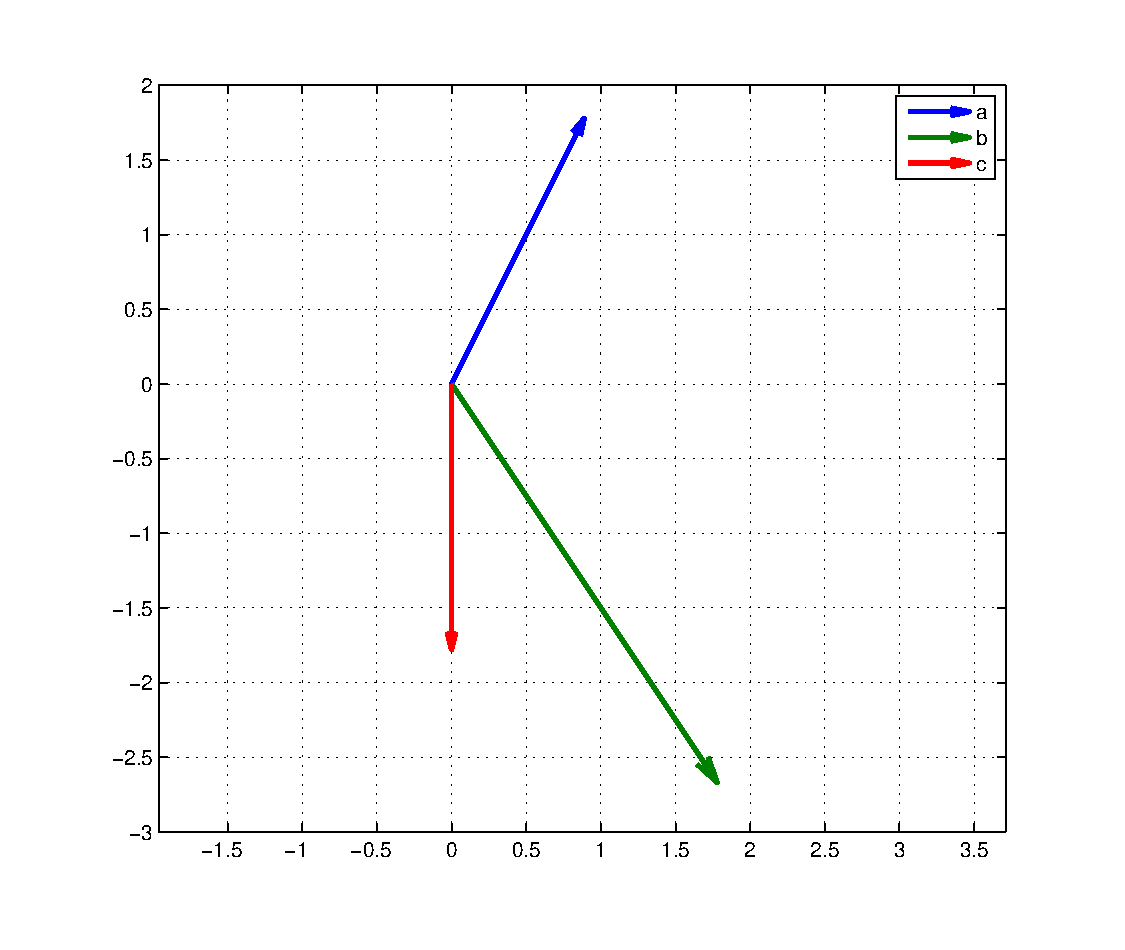
\includegraphics[width=7cm]{vectores.eps}
\bicaption{Representación gráfica de vectores en el plano}{Graphic of vectors on the plane}
\label{fig:vectores}
\end{figure}

\begin{paracol}{2}
De modo análogo, podemos asociar vectores de dimensión tres con puntos en el espacio tridimensional. En este caso, los valores de los elementos del vector corresponden con la coordenadas $(x,y,z)$ de los puntos en el espacio. La figura \ref{fig:vectores3} muestra la representación gráfica en espacio tridimensional de los vectores,
\switchcolumn
Likewise, we can associate vectors of dimension three with points in the 3D space. In this case, the vector entries represent the coordinates $(x,y,z)$ of the points in the space. Figure \ref{fig:vectores3} shows a graphic representation of vectors,
\end{paracol}
\begin{equation*}
a=
\begin{pmatrix}
1\\
2\\
1
\end{pmatrix},
b=
\begin{pmatrix}
2\\
-3\\
-1
\end{pmatrix},
c=
\begin{pmatrix}
0\\
-2\\
1
\end{pmatrix}
\end{equation*}

\begin{figure}[h]
\centering
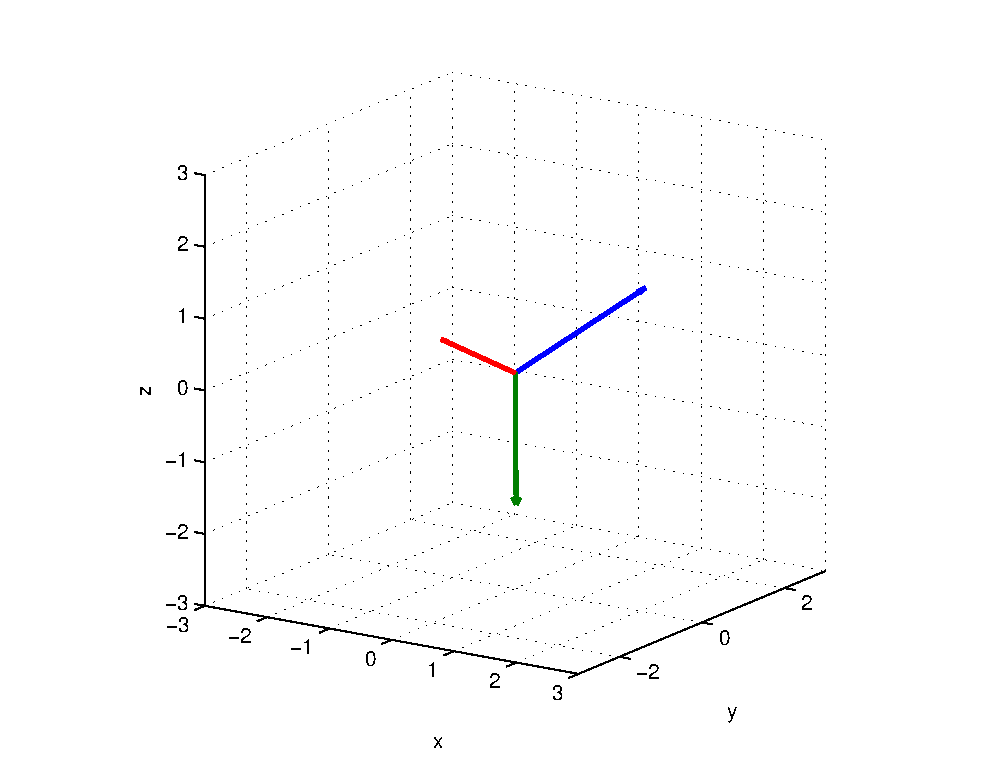
\includegraphics[width=9cm]{vectores3.eps}
\bicaption{Representación gráfica de vectores en el espacio 3D}{Graphic of vector in the 3D space}
\label{fig:vectores3}
\end{figure}
\begin{paracol}{2}
Evidentemente para vectores de mayor dimensión, no es posible obtener una representación gráfica. Si embargo muchas de las propiedades geométricas, observables en los vectores bi y tridimensionales, pueden extrapolarse a vectores de cualquier dimensión.

\subsection{Vectores y matrices en\\ Numpy.} \index{Vectores!en Numpy} \index{Matrices!en Numpy} 
\paragraph{Matrices.} Una de las característica más interesantes de Numpy, es la posibilidad de crear fácilmente matrices. Se pueden crear de diferentes maneras, la más elemental de todas ellas, emplea la funcion de Numpy \mintinline{python}{array} aplicada a una lista de filas de la matriz que se quiere construir. Cada fila debe ser a su vez una lista de números. Evidentemente, para que se pueda construir la matriz, todas las filas deben tener el mismo número de elementos. El siguiente ejemplo muestra como construir una matriz de dos filas y tres columnas,

\switchcolumn 
Obviously, it is impossible to get a graphic representation for vectors of larger dimensions. Nevertheless, many geometrical properties owned by 2D and 3D vectors can be applied to vectors of whatever dimension.

\subsection{Vectors and matrices in\\ Numpy.}\index[eng]{Vectors! in Numpy}\index[eng]{Matrices! in Numpy}
\paragraph{Matrices.} One interesting feature of numpy is that it allows us to create matrices easily. There are several methods to create them, but using the Numpy function \mintinline{python}{array} with a Python list with the rows of the matrix we want to build is probably the easiest method. Each row should be, in turn, a list of numbers, i.e., matrix entries. Of course, to build a matrix all rows should have the same number of entries. The following example shows how to build a matrix of two rows and three columns.
\end{paracol}

\begin{center}
    \begin{minipage}{0.4\textwidth}
    \begin{minted}{python}
In [3]: import numpy as np

In [4]: A = np.array([[1,2,3],[4,5,6]])

In [5]: print(A)
[[1 2 3]
 [4 5 6]]

In [6]: L = [[1,2,3],[4,5,6]]

In [7]: B = np.array(L)

In [9]: print(L)
[[1, 2, 3], [4, 5, 6]]

In [10]: print(B)
[[1 2 3]
 [4 5 6]]
 \end{minted}
\end{minipage}
 \end{center}
\begin{paracol}{2} 
Lo primero que hacemos es importar Numpy, lo importamos usando como alias la abreviatura np, porque es más cómodo a la hora de llamar a funciones específicas de Numpy.  Hemmos construido dos matrices iguales \mintinline{python}{A} y \mintinline{python}{B}. En el primer caso hemos creado directamente dentro de la llamada a la función \mintinline{python}{array}, la lista a partir de la cual construimos la matriz. En el segundo caso, hemos construido primero una lista \mintinline{python}{L}, y luego hemos empleado dicha lista como variable de entrada de la función \mintinline{python}{array}. Si nos fijamos en las líneas [9] y [10], vemos como Python distingue la lista ---todos sus elementos aparacen representados en la misma línea---, de la matriz en la que cada fila ocupa una línea distinta. Podemos construir matrices a partir de listas y variables ya definidas, siempre que seamos coherentes con el criterio de que cada fila se cree a partir de una lista y que todas las filas tengan los mismos elementos,
\switchcolumn
First, we import Numpy; we do it using \mintinline{python}{np} as an alias. The reason is that \mintinline{python}{np} is shorter than \mintinline{python}{numpy}, and it eases the calls to specific Numpy functions. We have built two identical matrices \mintinline{python}{a} and \mintinline{python}{B}. In the first case, we have straightforwardly created the list needed to make the matrix inside the call to the function \mintinline{python}{array}. In the second case, we first created a list \mintinline{python}{L}, and then we used it as an input variable to the function \mintinline{python}{array}. Focusing on lines [9] and [10], we see how Python can tell a list and a matrix apart. For a list, Python represents all entries in the same line. For a matrix, each row is written in a different line.
We can build matrices from lists and variables already defined as long as we follow the criteria that each row be created from a list and all rows have the same number of entries,  
\end{paracol}
\begin{center}
    \begin{minipage}{0.4\textwidth}
        \begin{minted}{python}
In [23]: a =1; b= 2; c =3

In [24]: d =[4,5,6]

        \end{minted}
\end{minipage}
\end{center}
\begin{center}
\begin{minipage}{0.4\textwidth}
\begin{minted}{python}
In [25]: C = np.array([[a,b,c],d])

In [26]: print(C)
[[1 2 3]
 [4 5 6]]

In [27]: C = np.array([[a,b,c],d,[7,8,9]])

In [28]: print(C)
[[1 2 3]
 [4 5 6]
 [7 8 9]]
        \end{minted}
    \end{minipage}
\end{center}
\begin{paracol}{2}
\paragraph*{Indexación.} \index{Numpy!indexación}Al igual que se hace en álgebra, Numpy es capaz de referirse a un elemento cualquiera de una matriz empleando índices para determinar su posición (fila y columna) dentro de la matriz.
\switchcolumn
\paragraph{Indexing}\index[eng]{Numpy!Indexing} As in algebra, in NUmpy is also possible to refer any entry of a matrix using indexes to indicate its position (row and column) in the matrix. 
\end{paracol}
\begin{equation*}
A=
\begin{pmatrix}
a_{11}&a_{12}&a_{13}\\
a_{21}&a_{22}&a_{23}\\
a_{31}&a_{32}&a_{33}
\end{pmatrix}
\end{equation*}

\begin{paracol}{2}
Sin embargo,  el criterio para referirse a un elemento concreto de una matriz, en Numpy está heredado de las listas: se indica el nombre de la variable que contiene la matriz y a continuación, entre corchetes y separados por una coma, el índice de su fila y después él de su columna \textbf{pero empezando a contar desde $0$}. Es decir, la primera fila de una matriz de dimensión $m\times n$ es la fila $0$ y la última es la fila $m-1$. De modo análogo su primera columna es la $0$ y su última columna es la $n-1$,
\switchcolumn
However, the Numpy criteria to refer to a specific entry inside a matrix has been borrowed from Python Lists: we write the name of the matrix followed by the row and column indexes of the entry we are interested in, enclosed in a square bracket and separated by a comma. The point is that we \textbf{count the rows and columns starting at $0$}. Thus, the first row of a matrix with dimensions $m\times n$ is the row $0$, and the last is the row $m-1$. Likewise, its first column is column $0$, and the last one is column $n-1$, 
\end{paracol}
\begin{center}
    \begin{minipage}{0.3\textwidth}
        \begin{minted}{python}
In [31]: print(C)
[[1 2 3]
 [4 5 6]
 [7 8 9]]

In [32]: C[1,2]
Out[32]: 6

In [33]: C[0,0]
Out[33]: 1
        \end{minted}
    \end{minipage}
\end{center}

\begin{paracol}{2}
Numpy puede seleccionar dentro de una matriz no solo elementos aislados, sino también submatrices completas. 
Para ello, emplea un símbolo reservado, el símbolo \emph{dos puntos} $:$. Este símbolo se emplea para recorrer valores desde un valor inicial hasta un valor final, con un incremento o paso fijo. La sintaxis es: \mintinline{python}{inicio:fin:paso}. Es importante tener en cuenta que Numpy detendrá la cuenta en el valor \mintinline{python}{stop-step}. Además, si no indicamos el tamaño del paso, Numpy tomará por defecto un paso igual a uno. En este caso basta emplear \mintinline{python}{start:stop}
\switchcolumn
Inside a matrix, Numpy can select single entries and whole submatrices. To do so, it uses the colon : symbol as a special symbol. Using a fixed step, we use this symbol to cover a set of values from a start (initial) value to a stop (final) one. The syntax is simple: \mintinline{python}{start:stop:step}. Beware! Numpy will stop the count in the step \mintinline{python}{stop-step}. Besides, if we leave apart the step size, Numpy will take a step equal to one. In this case, the expression is just \mintinline{python}{start:stop}
\end{paracol}

\begin{center}
        \begin{minted}{python}
In [87]: D = numpy.array([[1.,2.,3.],[4.,5.,6.],[-2,-3,0],[3,2,1]])

In [88]: print(D)
[[ 1.  2.  3.]
 [ 4.  5.  6.]
 [-2. -3.  0.]
 [ 3.  2.  1.]]

In [90]: D[0:1,0:3]
Out[90]: array([[1., 2., 3.]])

In [91]: D[0:2,0:2]
Out[91]: 
array([[1., 2.],
       [4., 5.]])

In [92]: D[2:3,1:2]
Out[92]: array([[-3.]])

In [93]: D[3:4,0:3]
Out[93]: array([[3., 2., 1.]])

In [94]: D[0:4,0:3]
Out[94]: 
array([[ 1.,  2.,  3.],
       [ 4.,  5.,  6.],
       [-2., -3.,  0.],
       [ 3.,  2.,  1.]])

In [95]: D[0:4,2:3]
Out[95]: 
array([[3.],
       [6.],
       [0.],
       [1.]])
       \end{minted}
\end{center}

\begin{paracol}{2}
La línea [90], extrae un vector fila con los elementos de la primera fila de la matriz \mintinline{python}{D}. La fila [91] extrae una matriz de dimension $2\times 2$ con los cuatro elementos de la esquina superior izquierda de la matriz original. La fila [92] extrae un único elemento pero sigue siendo una matriz de dimensión $1 \times 1$, por tanto es distinto que si empleamos la indexación directa del elemento: \mintinline{python}{D[2,1]}. La línea [93] nos devuelve un vector fila con la última fila de la matriz. La línea [94], nos devuelve de nuevo la matriz entera. Por último la línea [95] nos devuelve un vector columna con la primera columna de la matriz.

Hemos dicho que la línea [95] nos devuelve un vector columna. Bueno, sí y no; vamos a verlo más despacio.

\paragraph{Vectores.}
Cuando introducimos los vectores, distinguimos entre vectores filas y columna, definiéndolos como matrices de una sola fila o una sola columna. Sin embargo, en Numpy, se sigue un criterio distinto que permite generalizar el concepto de matriz asociándolo con el de tensor. Sin entrar en detalles\footnote{Una definición formal del concepto de tensor, queda fuera del alcance de estos apuntes.}, podemos decir que un tensor es un objeto algebráico caracterizado por dos parámetros; el orden y la dimensión. Así un escalar $a \in \mathbb{R}$ es un tensor de orden cero. Un vector $b \in \mathbb{R}^n$ es un tensor de orden 1 y dimesión $n$. Una matriz $A \in \mathbb{R}^{m\times n}$ Es un tensor de orden dos y dimensiones $m,n$. Un tensor de orden 3, $T \in \mathbb{R}^{n\times m \times l}$, etc. Podemos asociar el orden al número mínimo de índices que necesitamos para definir de forma unívoca los elementos de un Tensor: para un escalar, no nos hace faltar ningún indice, solo tenemos un elemento que es el propio escalar, por tanto le asociamos orden cero. Para un vector es suficiente emplear un índice para definir sus elementos, $b=(b_i),\ i=1,\cdots, n$, $b \in \mathbb{R}^n$. Para una matriz necesito dos índices, $A=(a_{ij}),\ i =1, \cdots n, j = 1,\ \cdots, m$, $A \in \mathbb{R}^{n\times m}$. Para un tensor de orden tres necesitaría tres índices, $T=(T_{ijk}),\ i =1,\cdots, n,\ j =1,\cdots m,\ k = 1,\cdots, l$, $T\in \mathbb{R}^{n\times m \times l}$ y así sucesivamente. Numpy permite definir estructuras de cualquier orden y dimensión que queramos. Pero nosotros nos vamos a limitar a vectores (orden 1) y matrices (orden 2). ¿Tiene sentido entonces distiguir entre vectores fila y columna? Solo si consideramos siempre los vectores como matrices (orden 2) y dimesiones $1\times n$ (vector fila) ó $n \times 1$ (vector columna). Para Numpy, sin embargo, vectores y matrices son estructuras de distinto orden. Veamos con algunos ejemplo cómo se diferencian. Para verlo mejor podemos emplear la propiedad \mintinline{python}{shape} de los arrays en numpy, Dicha propiedad nos devuelve una tupla con las dimensiones del array, el número de elementos que contine la tupla nos da el orden,
\switchcolumn
Line [90] extracts a row vector from the first row of matrix \mintinline{python}{D}. Line [91] extracts a $2\times 2$ matrix using the four entries located on the left-up corner of the original, \mintinline{python}{D}, matrix. Line [92] extracts a single matrix entry, but notice that it takes the form of a $1\times 1$ matrix. Thus, this result is different than the result achieved when we directly use the indexes of the entry: \mintinline{python}{D[2,1]}. Lain [93] returns a row vector with the entries of the matrix's last row. Lastly, line [95] returns a column vector with the entries of the matrix's last column.

We have said that line [95] returns a column vector. well, yes and not; let's see it in more detail.

\paragraph{Vectors.} When we introduced vectors in the previous section, we made a distinction between row and column vectors, defining them as matrices with a single row or a single column. Nevertheless, Numpy follows another criterion that allows us to generalise the idea of matrix linking it with the concept of tensor. we do not get into details\footnote{A formal definition of tensors is far beyond the scope of these notes.} and simply say that a tensor is an algebraic object defined by two parámeters, its order, and its dimension. So, a scalar $a \in \mathbb{R}$ is a tensor of order zero. A vector $b \in \mathbb{R}^n$ is a tensor of order one and dimension $n$. A matrix $A\in \mathbb{R}^{m\times n}$ is a tensor of order two and dimensions $m,n$. A third order tensor, $T\in\mathbb{R}^{n\times m\times l}$, etc. We can relate the order with the minimum number of indexes we need to univocally define the tensor entry: for a scalar, we don't need an index at all; we have only a single entry, the scalar itself. For this reason, we associate scalars with a zero-order tensor. For a vector, it is enough to use a single index to define its entries, $b=(b_i), i = 1,\cdots, n,\ b \in \mathbb{R}^n$. For a matrix, we need two indexes, $A = (a_{ij}), i =1,\dots,n,\ j = 1,\dots,m,\ A \in \mathbb{R}^{n\times m}$. For third-order tensors, we need three indexes, $T=(T_{ijk}),\ i =1,\cdots, n,\ j =1,\cdots m,\ k = 1,\cdots, l$, $T\in \mathbb{R}^{n\times m \times l}$ and so on. In Numpy, we can define structures of whatever order and dimensions we want, but we will only use vectors (order 1) and matrices (order 2). Has, then, any sense to distinguish between row and column vector? Only if we always consider vectors as matrices (order 2) and dimensions $1\times n$ (row vector) or $n\times 1$ (column vector). For Numpy, however, vectors an matrices are structures of different order. Let's see some examples of their differences. To appreciate it better we can use the Numpy arrays attribute \mintinline{python}{shape}, which gives us a tuple containing the dimensions of the array. The number of entries of the tuple tells us the order of the array,     
\end{paracol}
\begin{center}
    \begin{minipage}{0.3\textwidth}
    \begin{minted}{python}
In [23]: D
Out[23]: 
array([[ 1.,  2.,  3.],
       [ 4.,  5.,  6.],
       [-2., -3.,  0.],
       [ 3.,  2.,  1.]])

In [24]: D.shape
Out[24]: (4, 3)

In [25]: D[1,1]
Out[25]: 5.0

In [26]: D[1,1].shape
Out[26]: ()

In [27]: D[1,1:2]
Out[27]: array([5.])

In [28]: D[1,1:2].shape
Out[28]: (1,)
\end{minted}
\end{minipage}
\end{center}
\begin{center}
    \begin{minipage}{0.3\textwidth}
    \begin{minted}{python}
In [29]: D[1:2,1:2]
Out[29]: array([[5.]])

In [30]: D[1:2,1:2].shape
Out[30]: (1, 1)
    \end{minted}
        
    \end{minipage}
\end{center}

 \begin{paracol}{2}
 Empezamos con la matriz \mintinline{python}{D} de ejemplos anteriores. Para obtener sus dimensiones empleamos \mintinline{python}{D.shape}. El resultado es una tupla compuesta de dos elementos, puesto que es una matriz y, por tanto su orden es dos. El primer elemento no da la dimensión de sus columnas, es decir, el número de filas. El segundo elemento nos da la dimensión de sus filas, es decir el número de columnas. 
 
 En la línea [25] extraemos el elemento que ocupa la posición $[1,1]$. En la [26] cuando tratamos de obtener sus dimensiones, nos da una tupla vacía, porque es un escalar y su orden es cero. En la línea [27] le hemos pedido a Numpy que nos de los elementos de la fila $1$ de la matriz \mintinline{python}{D} que ocupan las columnas desde la $1$ hasta la $1$. Es decir, hacemos referencia al mismo elemento de la matriz, sin embargo el resultado no es exáctamente el mismo. Nos ha devuelto un array con el elemento seleccionado. Cuando el la línea [28] pedimos sus dimensiones, obtenemos una tupla con un único elemento \mintinline{python}{(1,)}. Es decir, el orden del array es $1$, se trata de un vector, y tiene de dimensión $1$, el vector solo tiene un elemento. 
 
 Por último, en la línea [29] volvemos a pedir a Python que nos de los elementos de la matriz \mintinline{python}{D}, que ocupan las filas desde la $1$ hasta la $1$ y las columnas desde la $1$ hasta la $1$, el resultado es ahora una matriz, podemos ver en la línea \mintinline{python}{out [29]} que el numero $5$ aparece ahora encerrado entre dos pares de corchetes. Cuando en la línea [30], preguntamos por su \mintinline{python}{shape}, nos devuelve una tupla con dos elementos --el orden del array es $2$, puesto que se trata de una matriz-- y sus dimensiones son una fila y una columna, puesto que la matriz solo tiene un elemento.  

 Vamos a completar nuestro estudio de los arrays en Python, extrayendo ahora partes más grandes de la misma matriz \mintinline{python}{D},
 \switchcolumn
 We begin with the same matrix \mintinline{python}{D} we use in previous examples. To get its dimensions, we use \mintinline{python}{D.shape}. The result is a tuple of two entries because it is a matrix, and thus, its order is two. The first entry gives us its column dimension, that is, its number of rows. The second entry is its row dimension, that is, its number of columns.

 In line [25] we extract the entry located at position $[1,1]$. In line [26] when we try to get its dimension, Numpy returns an empty tuple because it is a scalar and its order is zero. In line [27], we ask Numpy that retrieve the entries of row $1$ of the matrix \mintinline{python}{D} that fill the columns $1$ to $1$. Thus, we are making reference to the same entry of the matrix as in the previous case. However, the result is not exactly the same. Numpy retrieves an array with the selected entry. When we ask for its dimensions in line [28] we get a tuple with a single entry \mintinline{python}{(1,)}. Then, the order of the array is one. It is a vector with a single entry.

 Finally, in line [29], we ask Numpy to retrieve the entries of matrix \mintinline{python}{D} with fill the rows from $1$ to $1$ and the columns from $1$ to $1$. Thus, the result is now a matrix, We can see in line \mintinline{python}{out [29]} that the number $5$ is enclosed in two pair of square brackets. When in line [30], we ask for its \mintinline{python}{shape}, we get a tuple with two entries  --now the order of the array is two, because it is a matrix-- and their dimension are one row and one column as far as the matrix has a single entry.

 We are going to complete our study on Numpy arrays, extracting larger parts of the same matrix, 
 \end{paracol}
\begin{center}
 \begin{minipage}{0.3\textwidth}
    \begin{minted}{python}
In [9]: D
Out[9]: 
array([[ 1.,  2.,  3.],
       [ 4.,  5.,  6.],
       [-2., -3.,  0.],
       [ 3.,  2.,  1.]])

In [10]: D[1,:]
Out[10]: array([4., 5., 6.])

In [11]: D[:,1]
Out[11]: array([ 2.,  5., -3.,  2.])
    
In [12]: D[1:2,:]
Out[12]: array([[4., 5., 6.]])
\end{minted}
\end{minipage}
\end{center}
\begin{center}
 \begin{minipage}{0.3\textwidth}
    \begin{minted}{python}
In [13]: D[:,1:2]
Out[13]: 
array([[ 2.],
       [ 5.],
       [-3.],
       [ 2.]])
    \end{minted}
\end{minipage}
\end{center}
\begin{paracol}{2}
En el primer caso, línea [10], hemos extraido toda la segunda fila de la matriz \mintinline{python}{D}, el resultado es un vector, por tanto tiene orden $1$ y dimensión $3$. En la línea [11] hemos extraido la primera columna y el resultado es de nuevo un vector, por tanto tiene orden $1$ y la dimensión esta vez $4$. En la línea [12] extraemos todas las columnas de las filas que van desde la segunda hasta la segunda. El resultado es una matriz, ya que el orden del array extraído es $2$, y la dimensiones será $1$ para las filas y $3$ para las columna. Es lo más parecido a un vector 'fila' que podemos obtener con Numpy. Por último, en la línea [13], extraemos todas las filas de las columnas que van desde la segunda hasta la segunda. El resultado es de nuevo una matriz, porque el array extraido tiene orden dos, pero las dimensiones son ahora $4$ para las filas y $1$ para las columnas, lo podemos identificar con un vector columna de los descritos antes.

Evidentemente, podemos tambier extraer de una matriz bloque (submatrices), indicando las filas y columnas que queremos extraer de la matriz original. por ejemplo,
\switchcolumn
In the first case, line [10] we get the whole second row of matrix \mintinline{python}{D}. The result is a vector and has order $1$ and dimension $3$. In line [11], we extract the first column of the matrix, and the result is again a vector. This time the order is $1$, and the dimension is $4$. In line [12] we extract all columns belonging to rows second to second. The result is a matrix because the order of the extracted array is two. The dimensions are $1$ for the rows and $3$ for the columns. It is the most similar to a 'row' vector we can get using Numpy. Lastly, in line [13], we extract all the rows belonging to columns second to second. the result is again a matrix because the array obtained has order two, but the dimensions are now $4$ for the rows and $1$ for the columns, we could identify it as a column vector of those described above. 

Indeed, we can also  extract a block matrix (submatrices), using indexes to define the rows and columns we want to obtain from the original matrix,
\end{paracol}

\begin{center}
 \begin{minipage}{0.3\textwidth}
    \begin{minted}{python}
In [20]: D
Out[20]: 
array([[ 1.,  2.,  3.],
       [ 4.,  5.,  6.],
       [-2., -3.,  0.],
       [ 3.,  2.,  1.]])

In [21]: D[1:4,1:3]
Out[21]: 
array([[ 5.,  6.],
       [-3.,  0.],
       [ 2.,  1.]])

In [22]: D[1:3,0:2]
Out[22]: 
array([[ 4.,  5.],
       [-2., -3.]])
    \end{minted}
 \end{minipage}
\end{center}

\begin{paracol}{2}
\section{Operaciones matriciales}\label{opmatr} \index{Matrices! Operaciones Matriciales} 
A continuación definiremos las operaciones matemáticas más comunes, definidas sobre matrices. Vamos a empezar por aquellas que se realizan elemento a elemento, entre aquellos elementos que ocupan la misma posición en las matrices que se operan,

\paragraph{Suma.} La suma de dos matrices, se define como la matriz resultante de sumar los elementos que ocupan en ambas la misma posición. Solo está definida para matrices del mismo orden,

\switchcolumn
\section{Matrix Operations}\index[eng]{Matrices! Matrix Operations}
In this section we will define the most common mathematical operation for matrices. We are going to beging for those operation that are carried out, entry by entry, between those entries which occupy the same place in the operating matrices.

\paragraph{Addition.} Addition of two matrix, the result is a new matrix obtained adding the entries which ocuppy the same position in both matrices. It is denied only for matrix of the same dimensions, 

\end{paracol}
\begin{gather*}
C=A+B\\
c_{ij}=a_{ij}+b_{ij}\\
\\
\begin{pmatrix}
1& 2& 3\\
4& 5& 6\\
7& 8& 9\\
\end{pmatrix} =
\begin{pmatrix}
1& 3& 5\\
3& 5& 7\\
5& 7& 9\\
\end{pmatrix} +
\begin{pmatrix}
0& -1& -2\\
1& 0& -1\\
2& 1& 0\\
\end{pmatrix}
\end{gather*}
\begin{paracol}{2}
La suma de matrices cumple las siguientes propiedades,
\begin{enumerate}
\item Asociativa: $(A+B)+C=A+(B+C)$
\item Conmutativa: $A+B=B+A$
\item Elemento neutro: $O_{n\times m}+A_{n\times m}=A_{m\times m}$ El elemento neutro $O_{n\times m}$ de la suma de matrices de orden $n\times m$ es la matriz nula de dicho orden, ---compuesta exclusivamente por ceros--- . 
\item Elemento opuesto: La opuesta a una matriz se obtiene cambiando de signo todos sus elementos, $A_{op}=-A$
\end{enumerate}
En numpy el signo $+$ se también utiliza para representar la suma de matrices, por lo que la suma de dos matrices puede obtenerse directamente como,

\switchcolumn
Matrix addition fulfil the following properties,
\begin{enumerate}
\item Asociative: $(A+B)+C=A+(B+C)$
\item Conmutative: $A+B=B+A$
\item Identity element: $O_{n\times m}+A_{n\times m}=A_{m\times m}$ The identity element $O_{n\times m}$ of the addition of  $n\times m$ matrices is the null matriz of this dimensions, ---an only zeros matrix--- . 
\item Inverse: we get the addition inverse of a matrix changing the sings of all its entries $A_{inv}=-A$
\end{enumerate}
In numpy, the symbol $+$ also represents the matrix addition. Thus, you can use it to add two matrices in the same way you use it to add two numbers,
\end{paracol}

\begin{center}
    \begin{minipage}{.5\textwidth}
    \begin{minted}{python}
In [0]: import numpy as np
In [1]: A = np.array([[1,3,5],[2,4,6]])
In [2]: A
Out[2]: 
array([[1, 3, 5],
       [2, 4, 6]])

In [3]: B = np.array([[3,-2,0],[1,-4,3]])

In [4]: A+B
Out[4]: 
array([[4, 1, 5],
       [3, 0, 9]])

    \end{minted}
        
    \end{minipage}
\end{center}
\begin{paracol}{2}
En numpy, podemos crear una matriz de cualquier orden, compuesta exclusivamente por ceros mediante el comando\\ \mintinline{python}{numpy.zeros((m,n))}, donde $m$ es el número de filas y $n$ el de columnas de la matriz de ceros resultante. Si damos un único valor, \mintinline{python}{numpy.zeros(n)}, obtenedremos un vector formado por $n$ ceros.

\switchcolumn
We can use the Numpy command\\ \mintinline{python}{numpy.zeros((m,n))} to create a matrix, of whatever dimension, with all ist entries equal to zero. $m$ stands for the number of rows and $n$ for the number of columns of the zero matrix we want to create. If we use the command \mintinline{python}{numpy.zeros(n)} with a single value instead a tuple, then we will obtain a vector built up of $n$ zeros..  
\end{paracol}
\begin{center}
    \begin{minipage}{.3\textwidth}
        \begin{minted}{python}
In [375]: np.zeros(3)
Out[376]: array([0., 0., 0.])

In [377]: np.zeros((3,1))
Out[378]: 
array([[0.],
       [0.],
       [0.]])

In [379]: np.zeros((1,3))
Out[380]: array([[0., 0., 0.]])

In [381]: np.zeros((3,3))
Out[382]: 
array([[0., 0., 0.],
       [0., 0., 0.],
       [0., 0., 0.]])
       
In [383]: Z = np.zeros((2,3))

In [384]: A+Z
Out[385]: 
array([[1., 3., 5.],
       [2., 4., 6.]])
\end{minted}
    \end{minipage}
\end{center}
\begin{center}
    \begin{minipage}{.3\textwidth}
        \begin{minted}{python}       

In [386]: Aop = -A

In [387]: A+Aop
Out[388]: 
array([[0, 0, 0],
       [0, 0, 0]])
        \end{minted}
    \end{minipage}
\end{center}

\begin{paracol}{2}
\paragraph{Multiplicación elemento a elemento.} No es propiamente una operación matricial. Dadas dos matrices $A$ y $B$ de las mismas dimensiones, si las multiplicamos elemento a elemento, obtendremos una nueva matriz $C$ tal que, $c_{i,j} = a_{i,j}b_{i,j}$. Al igual que la suma, el producto elemento a elemento es asociativo y conmutativo. 
En Numpy el simbolo para la multiplicación elemento a elemento es el asterisco *,

\switchcolumn
\paragraph{entry-wise multiplication} This is not a proper matrix (algebraic) operation. You can get the entry-wise product of two matrices, $A$ and $B$, with the same dimensions to obtain a new matrix $C$ which entries are $c_{i,j} = a_{i,j}b_{i,j}$. This product, like the matrix addition, is conmutative and asociative. In numpy the entry-wise multiplication symbol is the asterisk *, 
\end{paracol}
\begin{center}
    \begin{minipage}{.5\textwidth}
        \begin{minted}{python}
In [49]: A
Out[49]: 
array([[1, 2],
       [2, 0],
       [3, 5]])

In [50]: B
Out[50]: 
array([[-3,  1],
       [ 0,  2],
       [ 1, -4]])

In [51]: A*B
Out[51]: 
array([[ -3,   2],
       [  0,   0],
       [  3, -20]])
\end{minted}
\end{minipage}
\end{center}
\begin{paracol}{2}
\paragraph{División elemento a elemento.} Es análoga a la multiplicación que acabamos de ver. Si dividimos elemento a elemento una matrix $A$ entre otra matriz $B$, ambas de las mismas dimensiones, obtenemos una matriz $C$ cuyos elementos cumplen $c_{ij} = a_{ij}/b_{ij}$. El símbolo que se emplea es el mismo de la división ordinaria entre números.

En el ejemplo siguiente, dividimos entre sí las dos matrices del ejemplo anterior, es interesante observar como Python nos advierte de la división entre cero, y asigna al elemento en que se produce el valor \mintinline{python}{inf}.

\switchcolumn
\paragraph{entry-wise division.} It is verymuch alike the elemet-wise product. If we divide entry-wise a matrix $A$ by another matrix $B$, both of the same dimensions, we get a new matrix $C$ which entries are $c_{ij}  = a_{ij}/b_{ij}$. For matrix entry-wise division, we use the same symbol as in the ordinamry number division.

In the following example, we divide the two matrix of the previous example, it is interesting to see how Python warnings us of a division by zero, and asigns to the resulting entry the value \mintinline{python}{inf}.
  

 
\end{paracol}
\begin{center}
    \begin{minipage}{\textwidth}
        \begin{minted}{python}
In [52]: A/B
/tmp/ipykernel_10098/713994841.py:1: RuntimeWarning: divide by zero encountered 
in divide A/B
Out[52]: 
array([[-0.33333333,  2.        ],
       [        inf,  0.        ],
       [ 3.        , -1.25      ]])
\end{minted}
\end{minipage}
\end{center}

\begin{paracol}{2}
\paragraph{Transposición.} Dada una matriz $A$, su transpuesta $A^T$ se define como la matriz que se obtiene intercambiando sus filas con sus columnas.
\switchcolumn
\paragraph{Transposition.} The transpose matrix $A^T$ of a matrix $A$ is the matrix we obtain intechanging its rows and columns.      
\end{paracol}


\begin{gather*}
A \rightarrow  A^T\\
a_{ij} \rightarrow  a_{ji}\\
A=
\begin{pmatrix}
1& -3& 2 \\
2& 7& -1
\end{pmatrix}  \rightarrow 
A^T=
\begin{pmatrix}
1& 2 \\
-3& 7\\
2 & -1
\end{pmatrix}
\end{gather*}

\begin{paracol}{2}
En numpy, la operación de transposición se indica mediante un punto y la letra T, \mintinline{python}{A.T}. Solo tiene sentido aplicarla para matrices; si transponemos un vector volvemos a obtener el mismo vector.
\switchcolumn
In Numpy the traspose matrix is obtained adding a point an the letter T to the matrix we wish to transpose, \mintinline{python}{A.T}. It only has sense for matrices. If we try to transpose a vector wi will optain the same vector again.
\end{paracol}

\begin{center}
    \begin{minipage}{0.5\textwidth}
        \begin{minted}{python}
In [375]: A
Out[375]: 
array([[1, 3, 5],
       [2, 4, 6]])

In [376]: A.T
Out[376]: 
array([[1, 2],
       [3, 4],
       [5, 6]])

In [377]: B = np.array([1,2,3]) 

In [378]: B.T
Out[378]: array([1, 2, 3])


In [379]: C = np.array([[1,2,3]])

In [380]: C
Out[380]: array([[1, 2, 3]])
        \end{minted}
    \end{minipage}
\end{center}
\begin{center}
    \begin{minipage}{0.5\textwidth}
        \begin{minted}{python}
In [381]: C.T
Out[381]: 
array([[1],
       [2],
       [3]])
        \end{minted}
    \end{minipage}
\end{center}

\begin{paracol}{2}
Una matriz cuadrada se dice que es simétrica si coincide con su transpuesta,
\switchcolumn
A square matrix is antisimetric if it is equal to its traspose matrix,
\end{paracol}

\begin{gather*}
A=A^T\\
a_{ij}=a{ji}\\
A=A^T=
\begin{pmatrix}
\ 1&\ 3&-3\\
\ 3&\ 0&-2\\
-3&-2&\ 4
\end{pmatrix}
\end{gather*}

\begin{paracol}{2}
Una matriz cuadrada es antisimétrica cuando cumple que $A=-A^T$. Cualquier matriz cuadrada se puede descomponer en la suma de una matriz simétrica más otra antisimétrica.

La parte simétrica puede definirse como,

\switchcolumn
A square matrix is antisimetric when it meets that $A=A^T$. Any square matrix can be split in the sum of two matrix, one simetric and another antisimetric

The simetric part can be defined as,
    
\end{paracol}
\begin{equation*}
A_S=\frac{1}{2} \left( A+A^T \right)
\end{equation*}

\begin{paracol}{2}
y la parte antisimétrica como,
\switchcolumn
An the antisimetric part as,   
\end{paracol}

\begin{equation*}
A_A=\frac{1}{2}\left( A-A^T \right)
\end{equation*}
\begin{paracol}{2}
Así, por ejemplo,
\switchcolumn
For instance,
\end{paracol}
\begin{equation*}
 A=A_S+A_A \rightarrow
\begin{pmatrix}
1& 2& 3\\
4& 5& 6\\
7& 8& 9\\
\end{pmatrix} =
\begin{pmatrix}
1& 3& 5\\
3& 5& 7\\
5& 7& 9\\
\end{pmatrix} +
\begin{pmatrix}
0& -1& -2\\
1& 0& -1\\
2& 1& 0\\
\end{pmatrix}
\end{equation*}
\begin{paracol}{2}
Por último, la transpuesta de la suma de matrices cumple,
\switchcolumn
The transpose of the addition of matrix meets,
\end{paracol}

\begin{equation*}
(A+B)^T=A^T+B^T
\end{equation*}

\begin{paracol}{2}
\paragraph{Producto de una matriz por un escalar.} El producto de una matriz $A$ por un número $b$ es una matriz del mismo orden que $A$, cuyos elementos se obtienen multiplicando los elementos de $A$ por el número $b$,
\switchcolumn
\paragraph{Product of a matrix and a scalar.} The product of a matrix $A$ for a number $b$ is a matrix with the same dimensions as $A$. We obtain the entry of this product multiplying the elemetns of $A$ by the number $b$,
\end{paracol}
\begin{gather*}
C=b\cdot A \rightarrow c_{ij}=b\cdot a_{ij}\\
3\cdot
\begin{pmatrix}
1& -2& 0\\
2& 3& -1&
\end{pmatrix}=
\begin{pmatrix}
3& -6& 0\\
6& 9& -3&
\end{pmatrix} 
\end{gather*}

\begin{paracol}{2}
En Python, el símbolo \mintinline{python}{*} se emplea también para representar el producto de una matriz por un número
\switchcolumn
In Python we also use the symbol \mintinline{python}{*} to represent the product of a matrix by a number.
\end{paracol}

\begin{center}
    \begin{minipage}{0.5\textwidth}
        \begin{minted}{python}
In [391]: A
Out[391]: 
array([[ 3, -5, -2,  1],
       [ 2,  3,  4,  5]])

In [394]: A*5
Out[394]: 
array([[ 15, -25, -10,   5],
       [ 10,  15,  20,  25]])
        \end{minted}
    \end{minipage}
\end{center}

\begin{paracol}{2}
\paragraph{Producto escalar de dos vectores.} Dados vectores de la misma dimensión $m$ se define su producto escalar como,
\switchcolumn
\paragraph{Dot product of two vectors}
For two vectors of the same dimension, we define the the dot product as,    
\end{paracol}


\begin{gather*}
a\cdot b=\sum_{i=1}^na_ib_i\\
\begin{pmatrix}
1\\
3\\
4
\end{pmatrix}\cdot
\begin{pmatrix}
1\\
-2\\
0
\end{pmatrix}
=1\cdot 1+3 \cdot (-2)+ 4 \cdot 0= -5
\end{gather*}
\begin{paracol}{2}
El resultado de producto escalar de dos vectores, es siempre un número; se multiplican los entre sí los elementos de los vectores que ocupan idénticas posiciones y se suman los productos resultantes. 

\paragraph{Producto matricial}
El producto de una matriz de orden $n\times m$ por una matriz $m\times l$, es una nueva matriz de orden $n\times l$, cuyos elementos se obtiene de acuerdo con la siguiente expresión,
\switchcolumn
The dot product result is always a number; we multiply the entry which take the same place in both vectors and then, we sum the resulting products. 

\paragraph{Matrix product} The matrix product of a $n \times m$ matrix by a $mtimes l$ matrix is a new matrix which dimensions are $n\times l$, We obtain the entries of the resulting matrix according with the following expression,    
\end{paracol}


\begin{equation*}
P=A\cdot B \rightarrow a_{ij}=\sum_{t=1}^m a_{it}b_{tj}
\end{equation*}
\begin{paracol}{2}
Por tanto, el elemento de la matriz producto que ocupa la fila $i$ y la columna $j$, se obtiene multiplicando por orden los elementos de la fila $i$ de la matriz $A$ con los elementos correspondientes de la columna $j$ de la matriz $B$, y sumando los productos resultantes

Para que dos matrices puedan multiplicarse es imprescindible que el número de columnas de la primera matriz coincida con el número de filas de la segunda.

Podemos entender la mecánica del producto de matrices de una manera más fácil si consideramos  la primera matriz como un grupo de vectores fila,

\switchcolumn
So, we get the entry of the product matrix which ocupies the the row $i$ and the column $j$, by multiplying in turn the entries of the row $i$ of matrix $A$ with the entries of the column $j$ of matrix $B$ and adding up the resulting products. 

Two matrix can be multiply only if the number of columns of the first matrix columns dimension is equal to the second matrix rows dimension.

We may understand better the matrix product mechanism if we consider the first matrix as a group of row vectors,  
\end{paracol}

\begin{equation*}
\begin{aligned}
A_1=\begin{pmatrix}
a_{11}& a_{12}& \cdots a_{1n}
\end{pmatrix}\\
A_2=\begin{pmatrix}
a_{21}& a_{22}& \cdots a_{2n}
\end{pmatrix}\\
\vdots \  \ \   \  \  \  \ \ \ \ \\
A_m=\begin{pmatrix}
a_{m1}& a_{m2}& \cdots a_{mn}
\end{pmatrix}
\end{aligned} \ \rightarrow \ 
A=\begin{pmatrix}
a_{11}& a_{12}& \cdots a_{1n}\\
a_{21}& a_{22}& \cdots a_{2n}\\
\vdots& \vdots& \cdots& \vdots \\
a_{m1}& a_{m2}& \cdots a_{mn}
\end{pmatrix}
\end{equation*}
\begin{paracol}{2}
y la segunda matriz como un grupo de vectores columna,
\switchcolumn
An the second matrix as a group of column vectors.  
\end{paracol}

\begin{equation*}
\begin{aligned}
B_1=\begin{pmatrix}
b_{11}\\ b_{21}\\ \vdots \\ b_{n1}
\end{pmatrix}&
B_2=\begin{pmatrix}
b_{12}\\ b_{22}\\ \vdots\\ b_{n2}
\end{pmatrix} &
\cdots  \  \  &
B_3=\begin{pmatrix}
b_{1m}\\ b_{2m}\\ \vdots  b_{nm}
\end{pmatrix}
\end{aligned} \ \rightarrow \ 
B=\begin{pmatrix}
b_{11}& b_{12}& \cdots b_{1n}\\
b_{21}& b_{22}& \cdots b_{2n}\\
\vdots& \vdots& \cdots& \vdots \\
b_{m1}& b_{m2}& \cdots b_{mn}
\end{pmatrix}
\end{equation*}

\begin{paracol}{2}
Podemos ahora considerar  cada elemento $p_{ij}$ de la matriz producto $P=A\cdot B$ como el producto escalar del vector fila $A_i$ for el vector columna $B_j$, $p_{ij}=A_i\cdot B_j$. 
Es ahora relativamente fácil, deducir algunas de las propiedad del producto matricial,

\begin{enumerate}
\item Para que dos matrices puedan multiplicarse, es preciso que el número de columnas de la primera coincida con el numero de filas de la segunda. Además la matriz producto tiene tantas filas como la primera matriz y tantas columnas como la segunda.

\item El producto matricial no es conmutativo. En general $A\cdot B \neq B \cdot A$

\item $(A\cdot B)^T=B^T\cdot A^T$
\end{enumerate}

\switchcolumn
we may consider the consider each entry $p_{ij}$ of the product matrix $P=A\cdot B$ as a escalar product of the row vector $A_i$ and the column vector $B_j$, $p_{ij} = A_i\cdot B_j$. Now we can easily find out some interesting properties of the matrix product.

\begin{enumerate}
\item Two matrices can be multiplyed only if the number of columns of the first matrix meet the number of columns of the second one. Besides, the product matrix has so meny row as the first matrix and so many columns as the second one.

\item Matrix produc it is not conmutative. In general, $A\cdot B \neq B \cdot A$

\item $(A\cdot B)^T=B^T\cdot A^T$
\end{enumerate}

\end{paracol}

\begin{paracol}{2}
En Numpy se emplea el símbolo \mintinline{python}{@} para representar el producto escalar, el producto de un vector por una matriz y el producto matricial. En todos los casos, es preciso que las dimensiones internas de los objetos que se multiplican coincidan. A continuación se muestran algunos ejemplos,

\switchcolumn
Numpy uses the symbol \mintinline{python}{@} to represent the scalar product, the product of a matrix and a vector and the matrix product. In any case, it is necessary that the inner dimensions of factor objects meet. Next we show some matrix multiplication examples, 
\end{paracol}
\begin{center}
    \begin{minipage}{0.7\textwidth}
        \begin{minted}{python}
In [382]: a = np.array([1,2,3,4])

In [383]: b = np.array([-1,2,0,-3])

In [384]: a@b
Out[384]: -9

In [386]: A = np.array([[3,-5,-2,1],[2,3,4,5]])

In [387]: A
Out[387]: 
array([[ 3, -5, -2,  1],
       [ 2,  3,  4,  5]])

In [388]: A@b
Out[388]: array([-16, -11])

In [389]: b@A.T
Out[389]: array([-16, -11])

        \end{minted}
    \end{minipage}
\end{center}
        
\begin{center}
    \begin{minipage}{0.7\textwidth}
        \begin{minted}{python}
        
In [390]: b@A
Traceback (most recent call last):

  Cell In[390], line 1
    b@A

ValueError: matmul: Input operand 1 has a mismatch in its core dimension 0, 
with gufunc signature (n?,k),(k,m?)->(n?,m?) (size 2 is different from 4)

In [398]: B
Out[398]: 
array([[ 0, -1],
       [-1,  0],
       [ 2,  3],
       [ 3,  4]])

In [399]: A@B
Out[399]: 
array([[ 4, -5],
       [20, 30]])

In [400]: B@A
Out[400]: 
array([[-2, -3, -4, -5],
       [-3,  5,  2, -1],
       [12, -1,  8, 17],
       [17, -3, 10, 23]])
        \end{minted}
    \end{minipage}
\end{center}

\begin{paracol}{2}
En la Línea In [384] se ha calculado el producto escalar de los vectores \mintinline{python}{a} y \mintinline{python}{b}. En este caso, la única condición requerida es que tengan la misma dimensión. En la línea In [388] se calcula el producto de la matriz \mintinline{python}{A} por el vector \mintinline{python}{b}. El requisito ahora es que la dimensión de la matriz ($2\times 4$), que corresponde al número de columnas, coincida con la única dimensión del vector ($4$). En la línea In [389] calculamos el producto del vector \mintinline{python}{b} por la transpuesta de la matriz \mintinline{python}{A}. La operación es posible porque la única dimensión del vector y coincide con la dimensión  de la matriz transpuesta $(4\time2)$, que corresponde con a número de filas. Sin embargo, no es posible calcular el producto del vector \mintinline{python}{b} por la matriz \mintinline{python}{A}, ya que la dimensión del vector no coincide con la primera dimensión de la matriz $(2\times4)$. En la línea In [399] hemos multiplicado las matrices \mintinline{python}{A} $(2\times 4$) por la matriz \mintinline{python}{B} $(4\times 2)$. Como coinciden las dimensiones ``internas'', --numero de columnas de la primera matriz con número de filas de la segunda-- La operación puede llevarse a cabo. Si invertimos el orden de las matrices, (línea In [400]) el producto también es posible, ya que en también coincidirían las dimensiones "internas". Sin embargo, es fácil ver que los resultados son complementamente distintos.
\switchcolumn
In line In[384] we calcuted the scalar product of vectors \mintinline{python}{a} and \mintinline{python}{b}. In this case, the only requirement is that both vector have the same dimension. In line In [388] we calculated the product of matrix \mintinline{python}{A} and the vector \mintinline{python}{b}. Now the requirement is the dimension of the matrix ($2\times 4$) correspondint to the number of columns, meets the the single dimension of the vector ($4$). In lin [389] we multiplied vector \mintinline{python}{b} with the traspose of matrix \mintinline{python}{A}. This operation can be carried uot because the single dimension of vector \mintinline{python}{b} is the same that the dimension of the traspose of the matrix $(4\times 2)$, which corresponds with the number of rows of the matrix. However, we cannot multiply vector \mintinline{python}{b} by matrix \mintinline{python}{A} because the dimension of the vector does not meet the first dimension of the matrix $(2\times 4)$. In line In [399] we multiplied matrix \mintinline{python}{A} $(2\times 4)$ by matix \mintinline{python}{B} $(4\times 2)$. We can carry out the operation because the ``inner'' dimensions of the matrices --number of columns of the first matrix and number of rows of the second one--, meet. If we invert the order of the matrices, (line In [400]) we can still multiply the matrix, because in this particular case the new ``inner'' also dimensions meet. However the result is entirely different        
\end{paracol}
\begin{paracol}{2}
\paragraph{Matriz identidad} La matriz identidad de orden $n\times n$ se 
define como:
\switchcolumn
\paragraph{The identity matrix } The identity matrix of dimension $n\times n$ is defined as:
\end{paracol}
\begin{equation*}
I_n= \left\{ 
\begin{aligned}
i_{ll}&=1\\
i_{kj}&=0, \ k\neq j
\end{aligned}
\right.
\end{equation*}

\begin{paracol}{2}
Es decir, una matriz en la que todos los elementos que no pertenecen a la diagonal principal son $0$ y los elementos de la diagonal principal son $1$. Por ejemplo,
\switchcolumn
So, an indentity matrix has any entry off the main diagonal equal to $0$ and all entries on the nain diagonal equal to $1$, for example,    
\end{paracol}

\begin{equation*}
I_3=\begin{pmatrix}
1& 0& 0\\
0& 1& 0\\
0& 0& 1
\end{pmatrix}
\end{equation*}

\begin{paracol}{2}
La matriz identidad $I_n$ es el elemento neutro del producto de matrices cuadradas de orden $n\times n$,
\switchcolumn
The indentity matrix $I_n$ is the identity element of the square $n \times n$ matrices product.    
\end{paracol}

\begin{equation*}
A_{n\times n}\cdot I_n=I_n\cdot A_{n\times n}
\end{equation*}
\begin{paracol}{2}
Además,
\switchcolumn
Besides,
\end{paracol}
\begin{gather*}
A_{n\times m}\cdot I_m=A_{n \times m}\\
I_n\cdot A_{n\times m}=A_{n\times m}
\end{gather*}

\begin{paracol}{2}
En Numpy se emplea el comando \mintinline{python}{eye(n)} para construir la matriz identidad de dimensiones $n\times n$,
\switchcolumn
In Numpy, we can use the command \mintinline{python}{eye(n)} to build the identity matrix of dimension $n\times n$.   
\end{paracol}

\begin{center}
    \begin{minipage}{0.3\textwidth}
        \begin{minted}{python}
In [381]: np.eye(4)
Out[381]: 
array([[1., 0., 0., 0.],
       [0., 1., 0., 0.],
       [0., 0., 1., 0.],
       [0., 0., 0., 1.]])
        \end{minted}
    \end{minipage}
\end{center}
\begin{paracol}{2}
Una matriz cuadrada se dice que es ortogonal si cumple,
\switchcolumn
An orthogonal matrix is a square matrix that fulfils,   
\end{paracol}
\begin{equation*}
A^T\cdot A=I
\end{equation*}

\begin{paracol}{2}
\paragraph{Norma de un vector.} La longitud euclídea, módulo,  norma 2 o simplemente norma  de un vector se define como,
\switchcolumn
\paragraph{Vector norm} The Euclidean length, module, norm 2 or just norm of a vector is defined as follows,
\end{paracol}
\begin{equation*}
\Vert x \Vert_2 =\Vert x \Vert =\sqrt{x\cdot x}=\sqrt{x^Tx}=\sqrt{x_1^2+x_2^2+\cdots x_n^2}=\left( \sum_{i=1}^nx_i^2 \right)^\frac{1}{2}
\end{equation*}
\begin{paracol}{2}
Constituye la manera usual de medir la longitud de un vector. Tiene una interpretación geométrica inmediata a través del teorema de Pitágoras: nos da la longitud del segmento que representa al vector. La figura \ref{fig:pitag} muestra dicha interpretación, para un vector bidimensional.

La norma de un vector en Numpy se obtiene empleando el  comando \mintinline{python}{norm} que pertenece al submódulo \mintinline{python}{linalg},
\switchcolumn
The vector norm represents the usual method to measure its length. It has a direct geometrical interpretation using Pithagoras' theorem: the norm is the length of the segment that represents the vector. Figure \ref{fig:pitag} shows such an interpretation for a bi-dimensional vector.
\end{paracol}
\begin{center}
    \begin{minipage}{0.3\textwidth}
        \begin{minted}{python}
In [422]: a
Out[422]: array([1, 2, 3, 4])

In [425]: np.linalg.norm(a)
Out[425]: 5.477225575051661
\end{minted}
\end{minipage}
\end{center}

\begin{figure}[h]
\centering
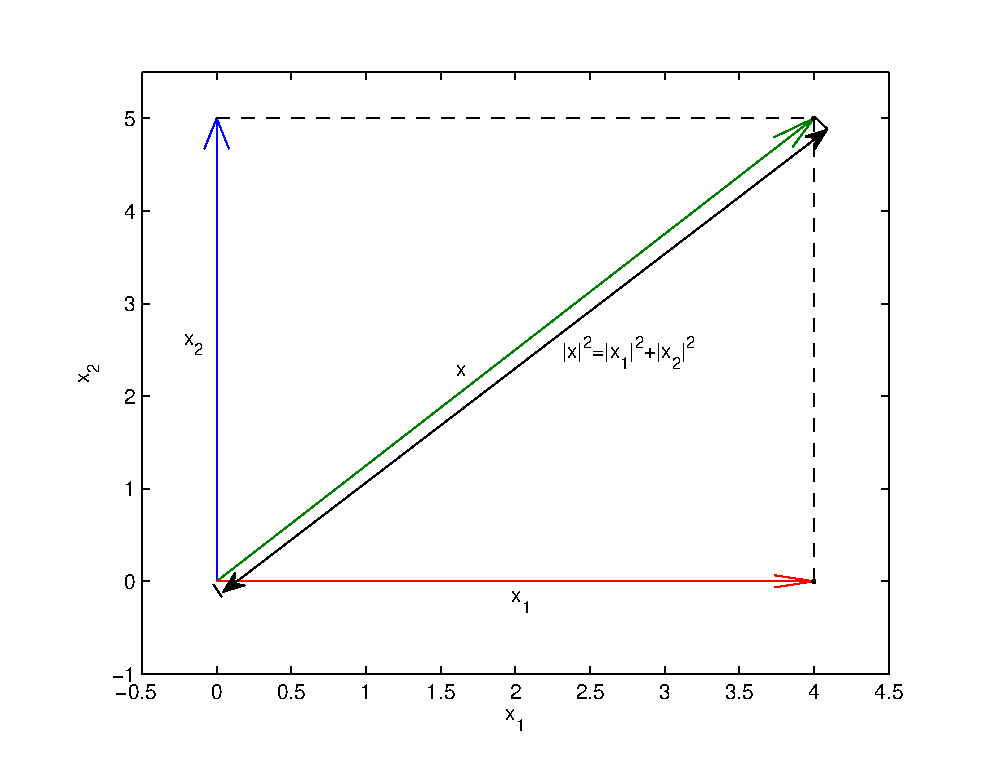
\includegraphics[width=12cm]{pitag.eps}
\bicaption{interpretación geométrica de la norma de un vector}{Geometrical interpretation of the norm of a vector.}
\label{fig:pitag}
\end{figure}
\begin{paracol}{2}
A partir de la norma de un vector es posible obtener una expresión alternativa para el producto escalar de dos vectores,
\switchcolumn
We can derive an alternative expression of the scalar product of two vector, using the vector norm
\end{paracol}
\begin{equation*}
a\cdot b=\Vert a \Vert \Vert b \Vert \cos \theta
\end{equation*}
\begin{paracol}{2}
Donde $\theta$ representa el ángulo formado por los dos vectores.
\switchcolumn
where $\theta$ is the angle between the two vectors.
\end{paracol}

\begin{flalign*}
&\mathwitch*_{i=0}^{\infty}\Xi_i(t)&     
\end{flalign*}

\begin{paracol}{2}
Aunque se trate de la manera más común de definir la norma de un vector, la norma 2 no es la única definición posible,

\emph{Norma 1:} Se define como la suma de los valores absolutos de los elementos de un vector,
\switchcolumn
Being the norm 2 the most common way to define a vector norm is by no means the only possible definition,

\emph{Norm 1:} defined as the sum of the absolute values of vector entries. 
\end{paracol}
\begin{equation*}
\Vert x \Vert_1 =\vert x_1\vert +\vert x_2 \vert\cdots \vert x_n\vert
\end{equation*}
\begin{paracol}{2}
\emph{Norma p:} Es una generalización de la norma 2,
\switchcolumn
\emph{P-Norm:} It is a generalization of the norm 2
\end{paracol}

\begin{equation*}
\Vert x \Vert_p =\sqrt[p]{\vert x_1^p\vert+\vert x_2^p\vert+\cdots \vert x_n^p\vert}=\left( \sum_{i=1}^n\vert x_i^p \vert \right)^\frac{1}{p}
\end{equation*}

\begin{paracol}{2}
\emph{Norma $\infty$:} se define como el mayor elemento del vector valor absoluto,
\switchcolumn
\emph{$\infty$ Norm:} The entry with the largest absolute value
\end{paracol}

\begin{equation*}
\Vert x \Vert_\infty =max \left\lbrace \vert x_i\vert\right \rbrace 
\end{equation*}

\begin{paracol}{2}
\emph{Norma $-\infty$:} el menor elemento del vector en valor absoluto,
\switchcolumn
\emph{$-\infty$ Norm:} The entry with the smallest absolute value. 
\end{paracol}
\begin{equation*}
\Vert x \Vert_{-\infty} =min \left\lbrace \vert x_i\vert\right \rbrace 
\end{equation*}
\begin{paracol}{2}
En Numpy la norma de un vector puede obtenerse mediante el comando \mintinline{python}{norm(v,p)}. La primera variable de entrada debe ser un vector y la segunda el tipo de norma que se desea calcular. Si se omite la segunda variable de entrada, el comando devuelve la norma 2. Para las normas $\infty\ \text{y} -\infty$ Se emplea el símbolo especial \mintinline{python}{inf} de Numpy. A continuación se incluyen varios ejemplo de utilización,
\switchcolumn
In Numpy the vector norm can be obtained using the command \mintinline{python}{norm(v,p)}. The first variable should be a vector and the second one represents the norm we want to calculate. If we leave out the second variable, the function returns norm 2 by default. For norms $\infty\ \text{y} \infty$ we use the symbol\mintinline{python}{inf} to represent the norm kind.
\end{paracol}

\begin{center}
    \begin{minipage}{.5\textwidth}
        \begin{minted}{python}
In [422]: a
Out[422]: array([1, 2, 3, 4])

In [423]: np.linalg.norm(a,1)
Out[423]: 10.0

In [424]: np.linalg.norm(a,2)
Out[424]: 5.477225575051661

In [425]: np.linalg.norm(a)
Out[425]: 5.477225575051661

In [426]: np.linalg.norm(a,4)
Out[426]: 4.337613136533361

In [427]: np.linalg.norm(a,np.inf)
Out[427]: 4.0

In [428]: np.linalg.norm(a,-np.inf)
Out[428]: 1.0
        \end{minted}
    \end{minipage}
\end{center}

\begin{paracol}{2}
En general, una norma se define como una función $\mathbb{R}^n \rightarrow \mathbb{R}$, que cumple,
\switchcolumn
In general, a norm can be define as functions $\mathbb{R}^n \rightarrow \mathbb{R}$, which satisfies,
\end{paracol}
\begin{align*}
&\Vert x\Vert \geq 0,\  \Vert x\Vert =0 \Rightarrow x=0\\
&\Vert x+y\Vert \leq \Vert x\Vert +\Vert y\Vert \\
&\Vert \alpha x\Vert = \vert \alpha \vert \Vert x\Vert ,\ \alpha \in \mathbb{R} 
\end{align*}

\begin{flalign*}
&&\reversemathwitch*    
\end{flalign*}

\begin{paracol}{2}
Llamaremos vectores unitarios $u$, a aquellos para los que se cumple que $\Vert u \Vert=1$.

Dos vectores $a$ y $b$ son ortogonales si cumplen que su producto escalar es nulo, $a^Tb=0 \Rightarrow  a\bot b$. Si además ambos vectores tienen módulo unidad, se dice entonces que los vectores son ortonormales.  Desde el punto de vista de su representación geométrica, dos vectores ortogonales, forman entre sí un ángulo recto.

\paragraph{Traza de una matriz.} La traza de una matriz cuadrada , se define como la suma de los elementos que ocupan su diagonal principal
\switchcolumn
Vectors $u$ with $\Vert u \Vert=1$ are called unitary vectors.

Two vectors $a$ and $b$ are orthogonal if their scalar product is zero, $a^Tb = 0 \Rightarrow a\bot b$. Besides, if the vectors have norm one them they are called orthonormal vectors. From the point of view of the geometrical representation, the angle between two orthogonal vectors is a square angle.

\paragraph{Matrix's trace.} The trace of a square matrix is the sum of the entries located in the matrix's main diagonal. 
\end{paracol}
\begin{gather*}
Tr(A)=\sum_{i=1}^na_{ii}\\
Tr\left(
\begin{pmatrix}
1& 4 & 4\\
2& -2 & 2\\
0& 3 & 6
\end{pmatrix}\right)=1-2+6=5
\end{gather*}

\begin{paracol}{2}
La traza de la suma de dos matrices cuadradas $A$ y $B$ del mismo orden, coincide con la suma de las trazas de $A$ y $B$,
\switchcolumn
The trace of the sum of two square, same dimension matrices $A$ and $B$ is equal to the sum of $A$ trace plus $B$ trace, 
\end{paracol}

\begin{equation*}
tr(A+B)=tr(A)+tr(B)
\end{equation*}

\begin{paracol}{2}
Dada una  matriz $A$ de dimensión $m\times n$  y una matriz $B$ de dimensión $n \times m$, se  cumple que,
\switchcolumn
For two matrices $A$ of dimensions $m\times n$ and $B$ of dimensions $n\times m$ is  always true that,
\end{paracol}

\begin{equation*}
tr(AB)=tr(BA)
\end{equation*}
\begin{paracol}{2}
En Python, puede obtenerse directamente el valor de la traza de una matriz $A$, mediante la función \mintinline{python}{np.trace(A)}. En este caso, se trata de un método asociado a cualquier array por lo que también puede expresarse como \mintinline{python}{A.trace()}  
\switchcolumn
In Numpy, the value of a matrix's trace can be calculated using the function \mintinline{python}{np.trace(A)}. In this case, the function is a method associated to any matrix and can be also expressed as \mintinline{python}{A.trace()}  
\end{paracol}

\begin{center}
\begin{minipage}{0.5\textwidth}
\begin{minted}{python}
In [197]: A = np.array([[1,2,3],[3,-2,3],[0,2,-1]])

In [198]: A
Out[198]: 
array([[ 1,  2,  3],
       [ 3, -2,  3],
       [ 0,  2, -1]])

In [199]: np.trace(A)
Out[199]: -2

In [200]: A.trace()
Out[200]: -2
\end{minted}
\end{minipage}
\end{center}


\begin{paracol}{2}
\paragraph{Determinante de una matriz.} 
En Numpy, el determinante de una matriz se calcula  empleando la función \mintinline{python}{det}, del submódulo \mintinline{python}{linalg}. Así, para calcular el determinante de la matriz $A$ del ejemplo anterior,
\switchcolumn
\paragraph{Matrix's determinant.} In Numpy, a matrix's determinant can be calculated using the function \mintinline{python}{det}, del submódulo \mintinline{python}{linalng}. We can calculate the determinant of matrix \mintinline{python}{A} of the previous example, 
\end{paracol}
\begin{center}
\begin{minipage}{0.5\textwidth}
\begin{minted}{python}
In [203]: np.linalg.det(A)
Out[203]: 20.000000000000007
\end{minted}
\end{minipage}
\end{center}

\begin{flalign*}
&\mathwitch*_{i=0}^{\infty}\Xi_i(t)&     
\end{flalign*}
\begin{paracol}{2}
El determinante de una matriz $A$, se representa habitualmente como $\vert A \vert$ o, en ocasiones como $det(A)$. Para poder definir el determinante de una matriz, necesitamos antes introducir una serie de conceptos previos. En primer lugar, si consideramos un escalar como una matriz de un solo elemento, el determinante  sería precisamente el valor de ese único elemento,
\switchcolumn
The determinant of a matrix, $A$ is usually represented as $\vert A\vert$ and occasionally as $det(A)$. To define the determinant of a matrix, we need first to establish some previous definitions. First, if we consider a scalar as a matrix of a single entry, the determinant of the matrix is this single entry.
\end{paracol}
\begin{equation*}
A=\begin{pmatrix}
a_{11}
\end{pmatrix} \rightarrow \vert A \vert =a_{11}
\end{equation*}
\begin{paracol}{2}
En álgebral lineal, se denomina menor primero, $M_{ij}$ de una matriz $A$, al determinate de la matriz que resulta de eliminar de la matriz $A$ la fila $i$ y la columna $j$. Por ejemplo,
\switchcolumn
In linear algebra, a first minor $M_{ij}$ of a square matrix $A$ is the determinant of the matrix obtained by removing simultaneously row $i$ and column $j$ of $A$. For instance, 
\end{paracol}

\begin{align*}
A=\begin{pmatrix}
1& 0& -2\\
3& -2& 3\\
0& 6& 5
\end{pmatrix},& \ 
M_{23}=det
\begin{pmatrix}
1& 0\\
0& 6
\end{pmatrix}\\
M_{32}=
det\begin{pmatrix}
1& -2\\
3& 3
\end{pmatrix},& \ 
M_{33}=
det\begin{pmatrix}
1& 0\\
3& -2
\end{pmatrix}\cdots
\end{align*}

\begin{paracol}{2}
 El  cofactor $C_{ij}$ de un elemento $a_{ij}$ de la matriz $A$, se define a partir del menor primero $M_{ij}$, que corresponde precísamenta a la fila y columna que contiene a $a_{ij}$,
 \switchcolumn
 We define the cofactor $C_{ij}$ of a matrix $A_{ij}$ entry, $a_{ij}$, using the first minor $M_{ij}$ obtained removing the row and column $a_{ij}$ belongs to.
\end{paracol}
 
\begin{equation*}
C_{ij}=(-1)^{i+j} M_{ij}
\end{equation*}

\begin{paracol}{2}
Podemos ahora definir el determinante de una matriz $A$ cuadrada de orden $n$, empleando la fórmula de Laplace,
\switchcolumn
Now, we can define the determinant of a $n$ dimensional square matrix $A$, using the Laplace's formula, 
\end{paracol}
\begin{equation*}
\vert A \vert = \sum_{j=1}^n a_{ij}C_{ij}
\end{equation*}
\begin{paracol}{2}
o alternativamente,
\switchcolumn
or also as,
\end{paracol}

\begin{equation*}
\vert A \vert = \sum_{i=1}^n a_{ij}C_{ij}
\end{equation*}
\begin{paracol}{2}
En el primer caso, se dice que se ha desarrollado el determinante a lo largo de la fila $i$. En el segundo caso, se dice que se ha desarrollo a lo largo de la columna $j$.

 La fórmula de Laplace obtiene el determinante de una matriz de orden $n\times n$ a partir del cálculo de los menores complementarios de los elementos de una fila o columna; los determinates the $n$ matrices de orden $(n-1)\times (n-1)$. A su vez, podríamos calcular cada menor complementario, aplicando la fórmula de Laplace y así sucesivamente hasta llegar a matrices de orden $2\times 2$. Para una matriz $2\times 2$, si desarrollamos por la primera fila obtenemos su determinante como,
\switchcolumn
In the first case, we say that we develop the determinant along the row $i$. In the second one, we say that we have developed the determinant along the column $j$

Laplace's formula gets the determinant of a Matrix of dimensions $n\times n$ using the first minors of a matrix row or column, i.e. the determinants of $n$ matrix of order $(n-1)\times (n-1)$. In turn, we can calculate each minor using Laplace's formula and so on, till we arrive at matrices of dimension $2\times 2$. We obtain the determinant of a $2\times 2$ matrix developing it along its first row,      

\end{paracol}

\begin{align*}
A&=\begin{pmatrix}
a_{11}& a_{12}\\
a_{21}& a_{22}
\end{pmatrix}\\
\vert A \vert & =\sum_{j=1}^2a_{1j}C_{1j} =a_{11}C_{11}+a_{12}C_{12}\\
 &=a_{11}(-1)^{1+1}\vert M_{11}\vert +a_{12}(-1)^{1+2}\vert M_{12}\vert \\
 &=-a_{11}a_{22}+a_{12}a_{21}\\
\end{align*}

\begin{paracol}{2}
y si desarrollamos por la segunda columna,
\switchcolumn
And if  we develop using the secon column,
\end{paracol}
\begin{align*}
A&=\begin{pmatrix}
a_{11}& a_{12}\\
a_{21}& a_{22}
\end{pmatrix}\\
\vert A \vert & =\sum_{j=1}^2a_{i2}C_{i2} =a_{12}C_{12}+a_{22}C_{22}\\
 &=a_{12}(-1)^{1+2}\vert M_{12}\vert +a_{22}(-1)^{2+2}\vert M_{22}\vert \\
 &=-a_{12}a_{21}+a_{22}a_{12}\\
\end{align*}

\begin{paracol}{2}
Para una matriz de dimensión arbitraria $n\times n$, el determinante se obtiene aplicando recursivamente la fórmula de Laplace,
\switchcolumn
For a matrix of arbitrary dimension we obtain the determinant using the Laplace's formula recursively,
\end{paracol}

\begin{align*}
&\vert A  \vert = \sum_{j=1}^na_{ij}C_{ij} =\sum_{j=1}^na_{ij}(-1)^{i+j} \left \vert M_{ij}^{(n-1)\times(n-1)} \right \vert \\
&\left \vert M_{ij}^{(n-1)\times(n-1)} \right \vert = \sum_{k=1}^{n-1}m_{lk}C_{lk} =\sum_{k=1}^{n-1}m_{lk}(-1)^{l+k} \left \vert M_{lk}^{(n-2)\times (n-2)} \right \vert\\
&\vdots \\
&\left \vert M_{st}^{1\times 1}\right \vert=(-1)^{s+t}m_{st} 
\end{align*}
\begin{paracol}{2}
Así, por ejemplo, podemos calcular el determinante de la matriz,
\switchcolumn
For instance, we can calculate the determinant of the following matrix,
\end{paracol}
\begin{equation*}
A=\begin{pmatrix}
1& 0& -2\\
3& -2& 3\\
0& 6& 5
\end{pmatrix}
\end{equation*}
\begin{paracol}{2}
desarrollándolo por los elementos de la primera columna, como,
\switchcolumn
Developing by the first column entries,
\end{paracol}
\begin{align*}
\left\vert A \right\vert =& 1\cdot (-1)^2\cdot 
\left\vert \begin{matrix}
-2& 3\\ 
6& 5
\end{matrix} \right\vert + 3\cdot (-1)^3\cdot
\left\vert \begin{matrix}
0& -2\\ 
6& 5
\end{matrix} \right\vert+ 0\cdot (-1)^4 \cdot 
\left\vert \begin{matrix}
0& -2\\ 
-2& -3
\end{matrix} \right\vert \\
=& 1\cdot (-1)^2\cdot \left[ (-2)\cdot 5 - 6\cdot 3 \right] +3\cdot (-1)^3\cdot  \left[ 0\cdot 5 - 6\cdot (-2)\right] + 0\cdot (-1)^4 \cdot \left[ 0\cdot 3 - (-2)\cdot (-2)\right]= -64
\end{align*}

\begin{paracol}{2}
Podemos programar en Python una función recursiva\footnote{El método no es especialmente eficiente pero ilustra el uso de funciones recursivas.} que calcule el determinante de una matriz de dimensiones $n\times n$.
\switchcolumn
We can now program a recursive function\footnote{The method is not particularly efficient but it helps to show the use of recursive functions} to calculate the determinant of any $n\times n$ dimensions.
\end{paracol}

\inputminted[
frame=lines,
framesep=2mm,
baselinestretch=1.2,
%bgcolor=LightGray,
label=determinante.py,
fontsize=\footnotesize,
linenos
]{python}{./codigos/Algebra/codigo_abierto/determinante.py}
\begin{flalign*}
&&\reversemathwitch*
\end{flalign*}
\begin{paracol}{2}
Entre las propiedades de los determinantes, destacaremos las siguientes,
\begin{enumerate}
\item El determinante del producto de un escalar $a$ por una matriz $A$ cumple,
\begin{equation*}
\left\vert a\cdot A \right\vert =a^n\cdot \vert A \vert
\end{equation*}
\item El determinante de una matriz es igual al de su traspuesta,
\begin{equation*}
\vert A \vert =\left\vert A^T \right\vert
\end{equation*}

\item El determinante del producto de dos matrices es igual al producto de los determinantes,
\begin{equation*}
\left\vert A_{n\times n} \cdot  B_{n\times n} \right\vert = \left\vert A_{n\times n} \right\vert \cdot \left\vert B_{n\times n} \right\vert 
\end{equation*}
\end{enumerate}

Una matriz es singular si su determinante es cero.

El rango de una matriz $A$ se define como el tamaño de la submatriz más grande dentro de $A$, cuyo determinante es distinto de cero. Así por ejemplo la matriz,
\switchcolumn
Among determinants' properties we will point out the following ones,
\begin{enumerate}
	\item The determint of a escalar $a$ by a  matrix $A$ is,
	\begin{equation*}
		\left\vert a\cdot A \right\vert =a^n\cdot \vert A \vert
	\end{equation*}
	\item The determinant of a matrix traspose equals the determinant of the matrix,
	\begin{equation*}
		\vert A \vert =\left\vert A^T \right\vert
	\end{equation*}
	
	\item The determinant of a matrix product equals the product of their determinants,
	\begin{equation*}
		\left\vert A_{n\times n} \cdot  B_{n\times n} \right\vert = \left\vert A_{n\times n} \right\vert \cdot \left\vert B_{n\times n} \right\vert 
	\end{equation*}
\end{enumerate}

A singular matrix is a square matrix whose determinant is zero.

The rank of a matrix $A$ is the size of the largest submatrix, inside $A$, whose determinant is non-zero. For instance,  
\end{paracol}
\begin{equation*}
A=\begin{pmatrix}
1& 2& 3\\
4& 5& 6\\
7& 8& 9
\end{pmatrix} \rightarrow \vert A \vert =0
\end{equation*}
\begin{paracol}{2}
Es una matriz singular y su rango es dos,
\switchcolumn
is a singular matrix, and its rank is 2,    
\end{paracol}

\begin{equation*}
\left \vert \begin{matrix}
1& 2\\
4& 5
\end{matrix} \right \vert=-3 \neq 0 \Rightarrow r(A)=2
\end{equation*}
\begin{paracol}{2}
Para una matriz cuadrada no singular, su rango coincide con su dimensión.

En Numpy se puede obtener el rango de una  matriz mediante el comando \mintinline{python}{matrix_rank},
\switchcolumn
For a non-singular square matrix, its rank meets its dimension.

In Numpy, we can obtain the rank of a matrix using the comand \mintinline{python}{matrix_rank},  
\end{paracol}
\begin{center}
\begin{minipage}{0.5\textwidth}
\begin{minted}{python}
In [395]: A
Out[395]: 
array([[1, 2, 3],
       [4, 5, 6],
       [7, 8, 9]])

In [396]: np.linalg.matrix_rank(A)
Out[396]: 2
\end{minted}
\end{minipage}
\end{center}
\begin{paracol}{2}
\paragraph{Inversión.} Dada una matriz cuadrada no singular $A$ de dimension $n$ existe una única matriz $A^{-1}$ de dimension $n$ que cumple,
\begin{equation*}
A\cdot A^{-1}=I_{n\times n}
\end{equation*}
Donde $I_{n\times n}$ es la matriz indentidad de dimensión $n$.
La matriz $A^{-1}$ recibe el nombre de matriz inversa de $A$, y  en numpy puede calcularse a partir de $A$ como \mintinline{python}{np.linalg.inv(A)}, ó \mintinline{python}{np.linalg.matrix_power(A,-1)}
En el segundo caso, estamos empleando la función, del submódulo linalg de numpy, \mintinline{python}{matrix.power(A,n)} que permite calcular el resultado de elevar una matriz a una pontencia $A^n$.
\switchcolumn
\paragraph{Inversion.} For a square non-singular matrix $A$ of dimension $n$ there is a unique matrix $A^{-1}$ of dimension $n$ that satisfies,
\begin{equation*}
	A\cdot A^{-1}=I_{n\times n}
\end{equation*}
Where $I_{n\times n}$ is the identity matrix of dimension $n$. The matrix $A^{-1}$ is called the inverse matrix of $A$, and we can calculate it in Numpy appliying the comands  \mintinline{python}{np.linalg.inv(A)}, ó \mintinline{python}{np.linalg.matrix_power(A,-1)} to the matrix $A$.
In the second case, we are using the function \mintinline{python}{matrix.power(A,n)} which allows us to calculate the result to raise a natrix to a power $A^n$. 
\end{paracol}
\begin{center}
\begin{minipage}{0.7\textwidth}
\begin{minted}{python}
In [409]: B = np.linalg.inv(A)

In [410]: B
Out[410]: 
array([[ 1.29166667, -0.58333333, -0.04166667],
       [ 0.58333333, -0.16666667, -0.08333333],
       [-0.48611111,  0.30555556,  0.06944444]])

In [411]: B @ A
Out[411]: 
array([[ 1.00000000e+00, -5.55111512e-17, -1.11022302e-16],
       [ 0.00000000e+00,  1.00000000e+00, -1.11022302e-16],
       [ 0.00000000e+00,  0.00000000e+00,  1.00000000e+00]])

In [412]: np.linalg.matrix_power(A,-1)
Out[412]: 
array([[ 1.29166667, -0.58333333, -0.04166667],
       [ 0.58333333, -0.16666667, -0.08333333],
       [-0.48611111,  0.30555556,  0.06944444]])
\end{minted}
\end{minipage}
\end{center}
\begin{flalign*}
&\mathwitch*_{i=0}^{\infty}\Xi_i(t) \lbrace &     
\end{flalign*}
\begin{paracol}{2}
La inversa de una matriz puede obtenerse a partir de la expresión,
\switchcolumn
A matrix inverse can be calculate using the following expression,
\end{paracol}
\begin{equation*}
A^{-1}=\frac{1}{\vert A \vert}[adj(A)]^T
\end{equation*}
\begin{paracol}{2}
Donde $adj(A)$ es la matriz adjunta de $A$, que se obtiene sustituyendo cada elemento $a_{ij}$ de $A$, por su cofactor $C_{ij}$. A continuación incluimos el código en Python de una función, \mintinline{python}{inver}, que calcula la inversa de una matriz. La función \mintinline{python}{inver} llama a su vez a la función \mintinline{python}{dumbdet} descrita más arriba, por lo que debemos importar el módulo \mintinline{python}{determinante} en el módulo en que vamos a crear la función \mintinline{python}{inver}.
\switchcolumn 
Where $adj(A)$ is the adjugate matrix of $A$, which can be obtained replacing each entry $a_{ij}$ of $A$ by its cofactor $C_{ij}$. Next, We include the Python code of a function, \mintinline{python}{inver}, to calculate the inverse of a matrix. The function \mintinline{python}{inver}, in turn,  calls the function \mintinline{python}{dumbdet}. Therefore, we must need to import the module \mintinline{python}{determinante} in the module where we will create the funtion \mintinline{python}{inver} 
\end{paracol}
\inputminted[
frame=lines,
framesep=2mm,
baselinestretch=1.2,
%bgcolor=LightGray,
label=inversa.py,
fontsize=\footnotesize,
linenos
]{python}{./codigos/Algebra/codigo_abierto/inversa.py}

\begin{flalign*}
&&\rbrace \reversemathwitch*
\end{flalign*}

\begin{paracol}{2}
Algunas propiedades relacionadas con la inversión de matrices son,
\begin{enumerate}
\item Inversa del producto de dos matrices,
\begin{equation*}
(A\cdot B)^{-1}=B^{-1}\cdot A^{-1}
\end{equation*}

\item Determinante de la inversa,
\begin{equation*}
\left\vert A^{-1} \right\vert = \vert A \vert ^{-1}
\end{equation*}

\item Una matriz es ortogonal si su inversa coincide con su transpuesta,
\begin{equation*}
A^{-1}=A^T
\end{equation*}
\end{enumerate}
\switchcolumn
Some properties relate with matrix inversion are,
\begin{enumerate}
	\item Inverse of the the producto of two matrices,
	\begin{equation*}
		(A\cdot B)^{-1}=B^{-1}\cdot A^{-1}
	\end{equation*}
	
	\item Determinant of the inverse matrix,
	\begin{equation*}
		\left\vert A^{-1} \right\vert = \vert A \vert ^{-1}
	\end{equation*}
	
	\item A matrix is ortogonal if its transpose is equal to its inverse,
	\begin{equation*}
		A^{-1}=A^T
	\end{equation*}
\end{enumerate}
\end{paracol}

\begin{table}[h]
\bicaption{Algunas funciones matemáticas en Numpy de uso frecuente}{frecuently used mathematical functions included in Numpy} \label{tabfun}

\begin{tabular}{c|c|c|c}
Tipo&Nombre&variables&función matemática\\
Type&Name&variables&funcion matemática\\
\hline
\hline

Trigonométricas&\multirow{2}{*}{cos}&\multirow{2}{4em}{y=cos(x)}&coseno de un ángulo en radianes\\
Trigonometric& & & Cosine of angle in radians\\
\hline
Trigonometricas&\multirow{2}{*}{sin}&\multirow{2}{4em}{y=sin(x)}&seno de un ángulo en radianes\\
Trigonometric& & &Sine of an angle in radians\\
\hline
Trigonométricas&\multirow{2}{*}{tan}&\multirow{2}{4em}{y=tan(x)}&tangente de un ángulo en radianes\\
Trigonometric & & &Tangent of an angle in radians\\
\hline
Trigonométricas &...&y=arc...(x)&inversa de una función trigonométrica\\
Trigonometric &arcsin&y=arcsin(x)& Inverse of a trigonometric function\\
\hline
\hline
Exponencial&\multirow{2}{*}{exp}&\multirow{2}{*}{y=exp(x)}&\multirow{2}{*}{$e^x$}\\
Exponential& & & \\
\hline
Exponencial&\multirow{2}{*}{log}&\multirow{2}{*}{y=log(x)}&logaritmo natural\\
Exponential & & & Natural logarithm\\
\hline
Exponencial&\multirow{2}{*}{log10}&\multirow{2}{*}{log10(x)}&logaritmo en base 10\\
Exponential& & & Basis 10 logarithm\\
\hline
Exponencial&\multirow{2}{*}{sqrt}&\multirow{2}{*}{y=sqrt(x)}&\multirow{2}{*}{$\sqrt{x}$}\\
Exponential& & & \\
\hline
\hline
Redondeo&\multirow{2}{*}{ceil}&\multirow{2}{*}{y=ceil(x)}& redondeo hacia $+\infty$\\
Rounding& & & rounding towards $+\infty$\\
\hline
Redondeo&\multirow{2}{*}{floor}&\multirow{2}{*}{y=floor(x)}&redondeo hacia $-\infty$\\
Rounding& & & rounding towards $-\infty$ \\
\hline
Redondeo&\multirow{2}{*}{rint}&\multirow{2}{*}{y=rint(x)}&redondeo al entero más próximo\\
Rounding& & & rounding towards the nearest integer\\
\hline
Redondeo&\multirow{2}{*}{fix}&\multirow{2}{*}{y=fix(x)}&redondeo hacia $0$\\
Rounding& & & rounding towards $0$\\
\hline
Redondeo&\multirow{2}{*}{mod}&\multirow{2}{*}{r=mod(x,y)}&resto de la división entera de y entre x\\
Rounding& & & remainder after integer division\\
\hline
\hline
Módulos&\multirow{2}{*}{norm}&\multirow{2}{*}{y=norm(x)}& módulo de un vector x\\
Norms & & & Norm of a vector\\
\hline
Módulos&\multirow{2}{*}{abs}&\multirow{2}{*}{y=abs(x)}&valor absoluto de x\\
Norms & & & Absolute value of x\\
\hline
Módulos&\multirow{2}{*}{sign}&\multirow{2}{*}{y=sign(x)}&función signo; 1 si x $>$ 0, -1 si x $<$ 0, 0 si x=0\\
Norms & & &sign function; 1 if x $>$ 0, -1 if x $<$ 0, 0 if x=0\\ 
\end{tabular}
\end{table}

\begin{paracol}{2}
\subsection{Funciones incluidas en\\ Num\-py.}\index{Funciónes! Funciones incluidas en Numpy} 
Numpy incluye un gran número de funciones. Muchas de ellas  están pensadas para ser aplicadas a arrays o a variables numéricas indistintamente. En el primer caso, la función se aplica elemento a elemento y el resultado es un array con las mismas dimensiones que el original. 

En la tabla \ref{tabfun}, se incluyen algunos ejemplos de las funciones matemáticas más corrientes. No están todas. Para obtener una visión más completa de las funciones disponibles se aconseja acudir a la documentacion de Numpy.
El uso de estas funciones es directo, por ejemplo, el siguiente código calcula la exponencial de los elementos de una matriz,
\switchcolumn
\subsection{Functions included in Numpy}\index{Functions! Funtions included in Numpy}
Numpy includes a large number of mathematical functions. Many of them are intended to be applied both, to arrays and simple variables. In the first case, the function is applied entry-wise and the result is an array with the same dimension than the original one.

Table \ref{tabfun} shows some examples of common mathematical functions. Not every function available in Numpy has been included. To achieve a complete view of available functions, it is advisable to read Numpy documentation.
These functions can be use straightforwardly, for instance, the following code calculates the exponential values of a matrix entries,   
\end{paracol}

\begin{center}
    \begin{minipage}{0.5\textwidth}
        \begin{minted}{python}
In [1]: import numpy as np

In [2]: A = np.array([[1,2],[2,0],[3,5]])

In [3]: A
Out[3]: 
array([[1, 2],
       [2, 0],
       [3, 5]])

In [4]: np.exp(A)
Out[4]: 
array([[  2.71828183,   7.3890561 ],
       [  7.3890561 ,   1.        ],
       [ 20.08553692, 148.4131591 ]])
        \end{minted}
    \end{minipage}
\end{center}

\begin{flalign*}
	&\mathwitch*_{i=0}^{\infty}\left\lbrace \right.&     
\end{flalign*}
\begin{paracol}{2}
\section{Operadores vectoriales}\label{opvect}
En esta sección vamos a estudiar el efecto de las operaciones matriciales, descritas en la sección anterior, sobre los vectores. Empecemos por considerar el producto por un escalar $\alpha \cdot a$. El efecto fundamental es modificar el módulo del vector,
\switchcolumn
\section{Vectorial operators}
In this section we will study the effect of matrix operation described in the previous section when they are applied to vectors. We start considering the effect if the product of a vector by a scalar $\alpha \cdot a$. The main effect is the change of the vector module,
\end{paracol}
\begin{equation*}
\alpha \cdot \begin{pmatrix}
a_1\\
a_2\\
a_3
\end{pmatrix}=
\begin{pmatrix}
\alpha a_1\\
\alpha a_2\\
\alpha a_3
\end{pmatrix}\rightarrow \vert \vert \alpha \cdot a \vert \vert =\sqrt{\alpha ^2a_1^2+\alpha ^2a_2^2+\alpha ^2a_3^2}=\vert \alpha \vert  \sqrt{a_1^2+a_2^2+a_3^2}=\vert \alpha \vert \cdot \vert \vert a \vert \vert
\end{equation*}
\begin{paracol}{2}
Gráficamente, si $\alpha$ es un número positivo y mayor que la unidad, el resultado del producto será un vector más largo que $a$ con la misma dirección y sentido. Si por el contrario, $\alpha$ es menor que la unidad, el vector resultante será más corto que $a$. Por último si se trata de un número negativo, a los resultados anteriores se añade el cambio de sentido con respecto a $a$. La figura \ref{fig:vmod} muestra gráficamente un ejemplo  del producto de un vector por un escalar.
\switchcolumn
If $\alpha$ is a positive number and greater than one, we observe graphically that the result of the product will be a vector larger than $a$ and with the same direction and sense. Conversely, if $\alpha$ is positive but less than one, the resulting vector will be shorter than $a$. Lastly if $\alpha$ is negative, a change of sense with respect to $a$ is added to the previously obtained results. Figure \ref{fig:vmod} shows graphically and example of the product of a vector by a scalar.
\end{paracol}
\begin{figure}[h]
\centering
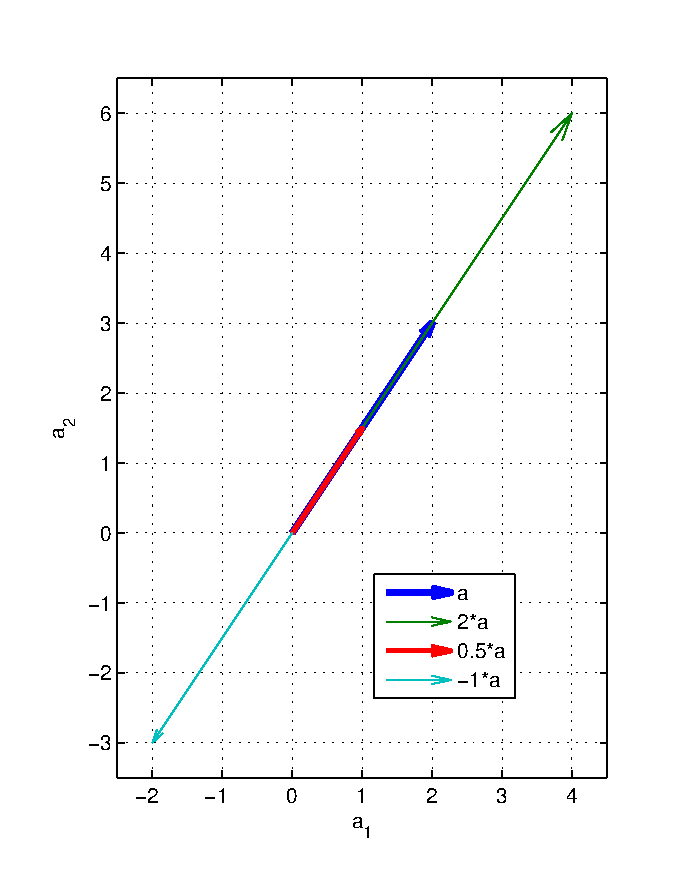
\includegraphics[width=7cm]{vmod.eps}
\bicaption{efecto del producto de un escalar por un vector}{effect of the product of a vector by a scalar}
\label{fig:vmod}
\end{figure}
\begin{paracol}{2}
\paragraph{Combinación lineal.} Combinando la suma de vectores, con el producto por un escalar, podemos generar nuevos vectores, a partir de otros, el proceso se conoce como combinación lineal,
\switchcolumn
\paragraph{Linear combination}Combining vector addition with product by a scalar, we can use a set of vectors to generate new vectors. This process is called linear combination. 
\end{paracol}
\begin{equation*}
c=\alpha \cdot a + \beta \cdot b + \cdots +\theta z
\end{equation*}
\begin{paracol}{2}
Así el vector $c$ sería el resultado de una combinación  lineal de los vectores $a, b, \cdots, z$. 
Dado un conjunto de vectores, se dice que son linealmente independientes entre sí, si no es posible poner a unos como combinación lineal de otros,
\switchcolumn
So, the vector $c$ is the result of linear combination of vectors $a,b,\cdots, z$.
A set o vectors are linearly independent if it is not possible to represent any of then as a combination of the others.
\end{paracol}

\begin{equation*}
\alpha \cdot a + \beta \cdot b + \cdots +\theta z=0 \Rightarrow \alpha =\beta =\cdots =\theta =0
\end{equation*}

\begin{paracol}{2}
Es posible expresar cualquier vector de dimensión $n$ como una combinación lineal de $n$ vectores linealmente independientes.

Supongamos $n=2$, cualquier par de vectores que no estén alineados, pueden generar todos los vectores de dimensión $2$ por ejemplo,
\switchcolumn
It is possible to represent any vector of dimensions $n$ as a lineal combination of $n$ vectors linearly independent.

Let's take $n=2$,  any pair of no collinear vectors can generate all vectors of dimension $2$, for example,
\end{paracol}

\begin{equation*}
\begin{pmatrix}
x_1\\
x_2
\end{pmatrix}=
\alpha \begin{pmatrix}
1\\
2
\end{pmatrix}+\beta \begin{pmatrix}
-1\\
1
\end{pmatrix}
\end{equation*}



\begin{figure}[h]
\centering
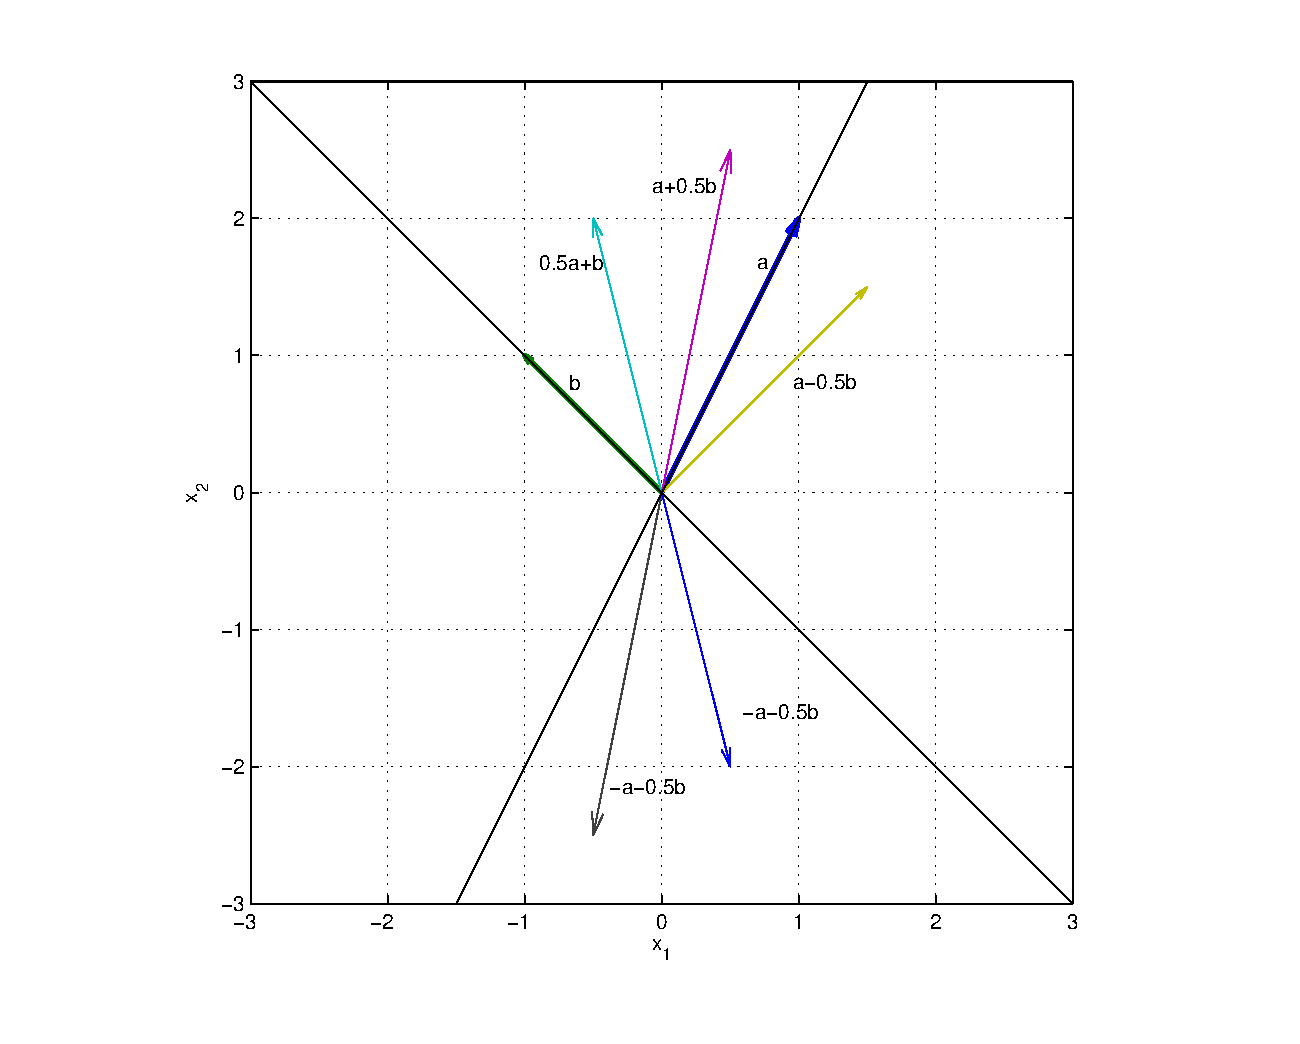
\includegraphics[width=10cm]{clineal.eps}
\bicaption{Representación gráfica de los vectores $a=(1,2)$, $b=(-1,1)$ y algunos vectores, combinación lineal de $a$ y $b$.}{A graphic representations of Vectors $a=(1,2)$, $b=(-1,1)$ and some vectors obtained from a lineal combination of $a$ and $b$.}
\label{fig:clineal}
\end{figure}

\begin{paracol}{2}
La figura \ref{fig:clineal} muestra gráficamente estos dos vectores y algunos de los vectores resultantes de combinarlos linealmente.

Si tomamos como ejemplo $n=3$, cualquier conjunto de vectores que no estén contenidos en el mismo plano, pueden generar cualquier otro vector de dimensión $3$. Por ejemplo,

\switchcolumn
Figure \ref{fig:clineal} shows these two vector and some other vectors obtained by combining them linearly.

If we take now $n=3$, whatever three vectors not contained in the same plane can generate any other vector of dimension three. For example,
\end{paracol}

\begin{equation*}
\begin{pmatrix}
x_1\\
x_2\\
x_3
\end{pmatrix}=\alpha \begin{pmatrix}
1\\
-2\\
1
\end{pmatrix}+ \beta \begin{pmatrix}
2\\
0\\
-1
\end{pmatrix}+ \gamma \begin{pmatrix}
-1\\
1\\
1
\end{pmatrix}
\end{equation*}

\begin{paracol}{2}
La figura \ref{fig:clin3} muestra gráficamente estos tres vectores y el vector resultante de su combinación lineal, con $\alpha=1$, $\beta=-0.5$ y $\gamma=1$.  Es fácil ver a partir de la figura que cualquier otro vector de dimensión $3$ que queramos construir puede obtenerse a partir de los vectores $a$, $b$ y $c$.
\switchcolumn
Figure \ref{fig:clin3} shows these three vector and another one obtained by combining them linearly, taking $\alpha=1$, $\beta=-0.5$ y $\gamma=1$. It is easy to deduce using the figure thar any other three-dimensional vector can be built using vectors $a$, $b$ y $c$.
\end{paracol}

\begin{figure}
\centering
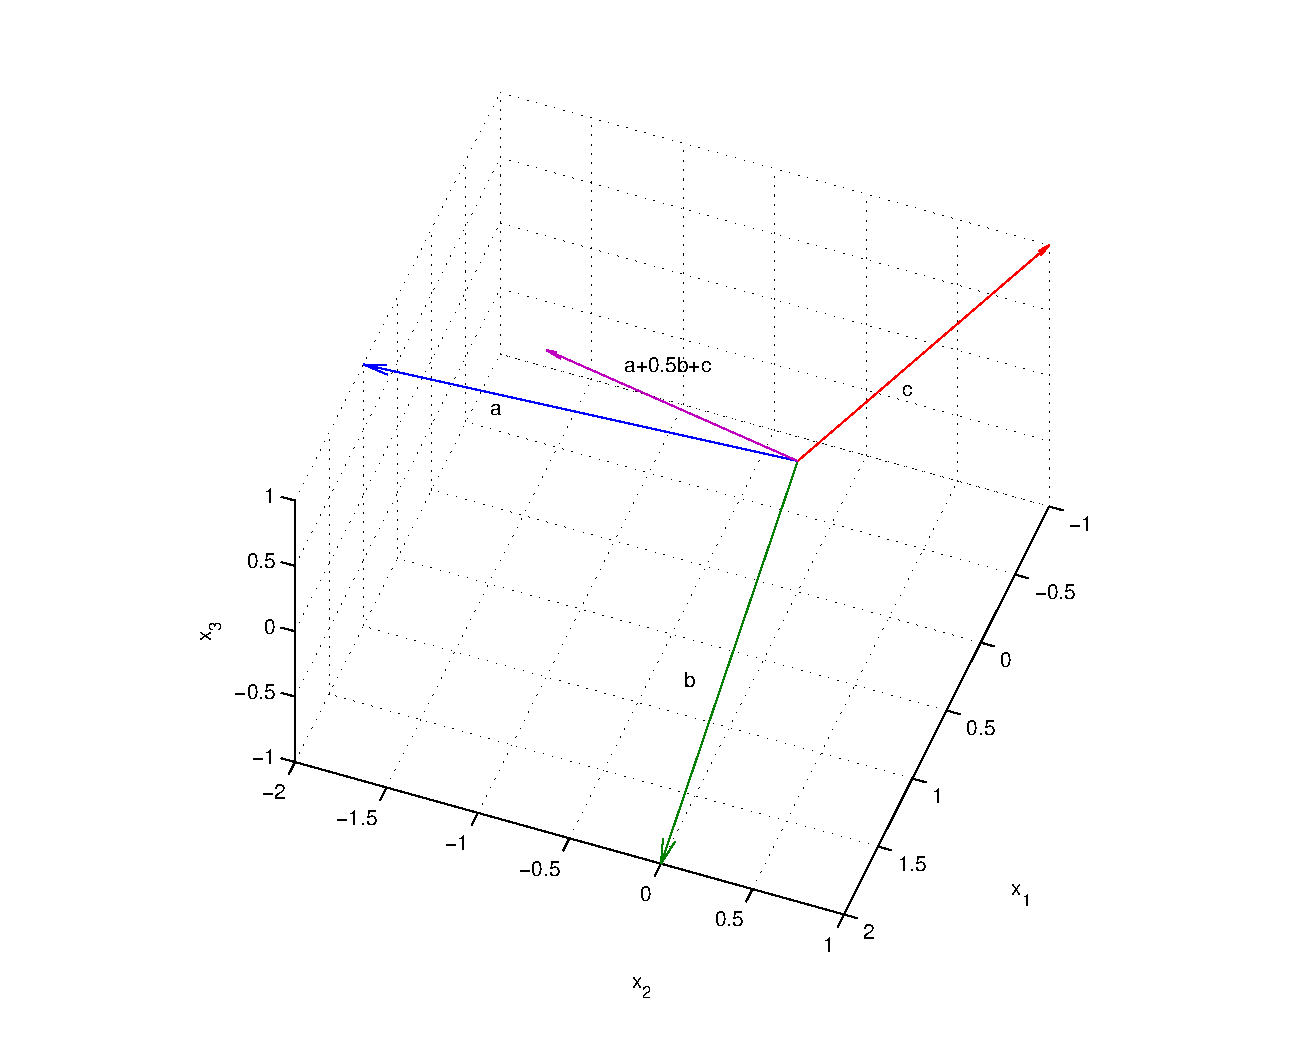
\includegraphics[width=12cm]{clin3.eps}
\bicaption{Representación gráfica de los vectores $a=(1,-2,1)
$, $b=(2,0,-1)$, $c=(-1,1,1)$ y del vector $a-b+c$.}{Vectors $a=(1,-2,1)$, $b =(2,0-1))$, $c=(-1,1,1)$ and vector $a-b+c$; a graphic representation}
\label{fig:clin3}
\end{figure}

\begin{paracol}{2}
\paragraph{Espacio vectorial y  bases del espacio vectorial.} El conjunto de los vectores de dimensión $n$, junto con la suma vectorial y el producto por un escalar, constituye  un  \emph{espacio vectorial} de dimensión $n$.

 Como acabamos de ver, es posible obtener cualquier vector de dicho espacio vectorial a partir de $n$ vectores linealmente independientes del mismo. Un conjunto de $n$ vectores linealmente independientes de un espacio vectorial de dimensión $n$ recibe el nombre de base del espacio vectorial. En principio es posible encontrar infinitas bases distintas para un espacio vectorial de dimensión $n$. Hay algunas particularmente interesantes,
 
 \subparagraph{Bases ortogonales.} Una base ortogonal es aquella en que todos sus vectores son ortogonales entre sí , es decir cumple que su producto escalar es $b^i\cdot b^j=0, i\neq j$. Donde  $b^i$ representa el \emph{i-ésimo} vector de la base, $\mathcal{B}=\left\lbrace b^1, b^2, \cdots, b^n  \right\rbrace $ .
 
 \subparagraph{Bases ortonormales.} Una base ortonormal, es una base ortogonal en la que, además, los vectores de la base tienen módulo $1$. Es decir, $b^i\cdot b^j=0, i\neq j$ y  $b^i\cdot b^j=1, i = j$. Un caso particularmente útil de base ortonormal es la base canónica, formada por los vectores, 
\switchcolumn
\paragraph{Vector spaces and vector space bases.} 

The set of all $n$-dimensional vectors with the vector addition and the product by scalars define a \emph{vector space} of dimension $n$.

 We have already seen that it is possible to obtain any vector of this $n$-dimensional space using $n$ linearly independent vectors belonging to the space. A set of $n$ linearly independent vector in a vector space of dimension $n$, is called a basis of the vector space. We can, in principle, find infinity different basis for an $n$-dimensional vector space. Some of these bases have properties that make them specially interesting,
 
 \subparagraph{Ortogonal bases.} An ortogonal basis is built by vectors which are all ortogonal among then. That is, the scalar product is $b^i\cdot b^j =0,\ i \neq j$. Where $b^i$ is the $i$ vector of the basis, $\mathcal{B} =\left\lbrace b^1,b^2,\cdots,b^n \right\rbrace$.

\subparagraph{Ortonormal bases.} An ortogonal basis whose vectors, in addition,  have norm $1$ is called an ortonormal basis. That is, $b^i\cdot b^j=0, i\neq j$ and  $b^i\cdot b^j=1, i = j$. A particularly useful ortonormal basis is the canonical basis, composed by the following vectors, 
\end{paracol}

\begin{equation*}
\mathcal{C}=\left\lbrace c^1=\begin{pmatrix}
1\\
0\\
0\\
\vdots \\
0
\end{pmatrix}, c^2=\begin{pmatrix}
0\\
1\\
0\\
\vdots \\
0
\end{pmatrix},
\cdots
c^{n-1}=\begin{pmatrix}
0\\
0\\
\vdots \\
1\\
0
\end{pmatrix},
c^n=\begin{pmatrix}
0\\
0\\
\vdots \\
0\\
1
\end{pmatrix} \right\rbrace
\end{equation*} 
\begin{paracol}{2}
Podemos considerar las componentes de cualquier vector como los coeficientes de la combinación lineal de la base canónica que lo representa,
\switchcolumn
We can consider the components of any vector as the coefficients of the linear combination of the canonical base vectors which represents the vector
\end{paracol}
\begin{equation*}
a=\begin{pmatrix}
a_1\\
a_2\\
\cdots  \\
a_{n-1}\\
a_n
\end{pmatrix} =a_1\cdot \begin{pmatrix}
1\\
0\\
0\\
\vdots \\
0
\end{pmatrix}+a_2 \cdot  \begin{pmatrix}
0\\
1\\
0\\
\vdots \\
0
\end{pmatrix}+
\cdots +
a_{n-1}\cdot \begin{pmatrix}
0\\
0\\
\vdots \\
1\\
0
\end{pmatrix}+
a_n\cdot \begin{pmatrix}
0\\
0\\
\vdots \\
0\\
1
\end{pmatrix}
\end{equation*}

\begin{paracol}{2}
Por extensión, podemos generalizar este resultado a cualquier otra base, es decir podemos agrupar en un vector los coeficientes de la combinación lineal de los vectores de la base que lo generan. Por ejemplo, si construimos, para los vectores de dimensión $3$ la base,
\switchcolumn
We can also generalise and extend this result to any other basis, just grouping in a vector the coeficients of linear combination of basis vectors which generates it. For example, we can build for vector of dimension $3$ the following basis,   
\end{paracol}

\begin{equation*}
\mathcal{B}=\left\lbrace \begin{pmatrix}
1\\
2\\
0
\end{pmatrix}, \begin{pmatrix}
-1\\
0\\
2
\end{pmatrix}, \begin{pmatrix}
1\\
-1\\
1
\end{pmatrix} \right\rbrace
\end{equation*} 
\begin{paracol}{2}
Podemos entonces representar un vector en la base $\mathcal{B}$ como,
\switchcolumn
We can then represent a vector in the basis $\mathcal{B}$ as,
\end{paracol}

\begin{equation*}
\alpha \cdot \begin{pmatrix}
1\\
2\\
0
\end{pmatrix}+\beta \cdot \begin{pmatrix}
-1\\
0\\
2
\end{pmatrix}+ \gamma \cdot \begin{pmatrix}
1\\
-1\\
1
\end{pmatrix} \rightarrow a^{\mathcal{B}}=\begin{pmatrix}
\alpha \\
\beta \\
\gamma
\end{pmatrix}
\end{equation*} 
\begin{paracol}{2}
Donde  estamos empleando el superíndice $^{\mathcal{B}}$, para indicar que las componentes del vector $a$ están definidas con respecto a la base $\mathcal{B}$.

Así por ejemplo el vector,
\switchcolumn
Where the superscript $^\mathbb{B}$, means that vector $a$ components are defined in basis $\mathcal{B}$.

So, for instance, vector,
\end{paracol} 
\begin{equation*}
a^{\mathcal{B}}=\begin{pmatrix}
1.125\\
0.375\\
0.75
\end{pmatrix}
\end{equation*}
\begin{paracol}{2}
Tendría en la base canónica las componentes,
\switchcolumn
Would have the following component in the canonical basis,
\end{paracol}
\begin{equation*}
a^{\mathcal{B}}=\begin{pmatrix}
1.125\\
0.375\\
0.75
\end{pmatrix} \rightarrow a= 1.125 \cdot \begin{pmatrix}
1\\
2\\
0
\end{pmatrix}+0.375 \cdot \begin{pmatrix}
-1\\
0\\
2
\end{pmatrix}+ 0.75 \cdot \begin{pmatrix}
1\\
-1\\
1
\end{pmatrix} =\begin{pmatrix}
1.5\\
1.5 \\
1.5
\end{pmatrix}
\end{equation*}

\begin{paracol}{2}
La figura \ref{fig:base1}, muestra gráficamente la relación entre los vectores de la base canónica $\mathcal{C}$, los vectores de la base $\mathcal{B}$, y el vector $a$, cuyas componentes se han representado en ambas bases.

Podemos aprovechar el producto de matrices para obtener las componentes en la base canónica $\mathcal{C}$ de un vector representado en una base cualquiera $\mathcal{B}$. Si agrupamos los vectores de la base $\mathcal{B}$, en una matriz $B$,
\switchcolumn
Figure \ref{fig:base1}, shows the relationship among the canonical basis vectors $\mathcal{C}$, the basis $\mathcal{B}$ vectors, and vector $a$, whose component have been represented in both bases.

We can use the matrix product to obtain any vector components in the canonical basis $\mathcal{C}$ from the vector components in any other basis $\mathcal{B}$. If we put together the basis $\mathcal{B}$ vector in a single matrix $B$,
\end{paracol}
\begin{figure}[h]
\centering
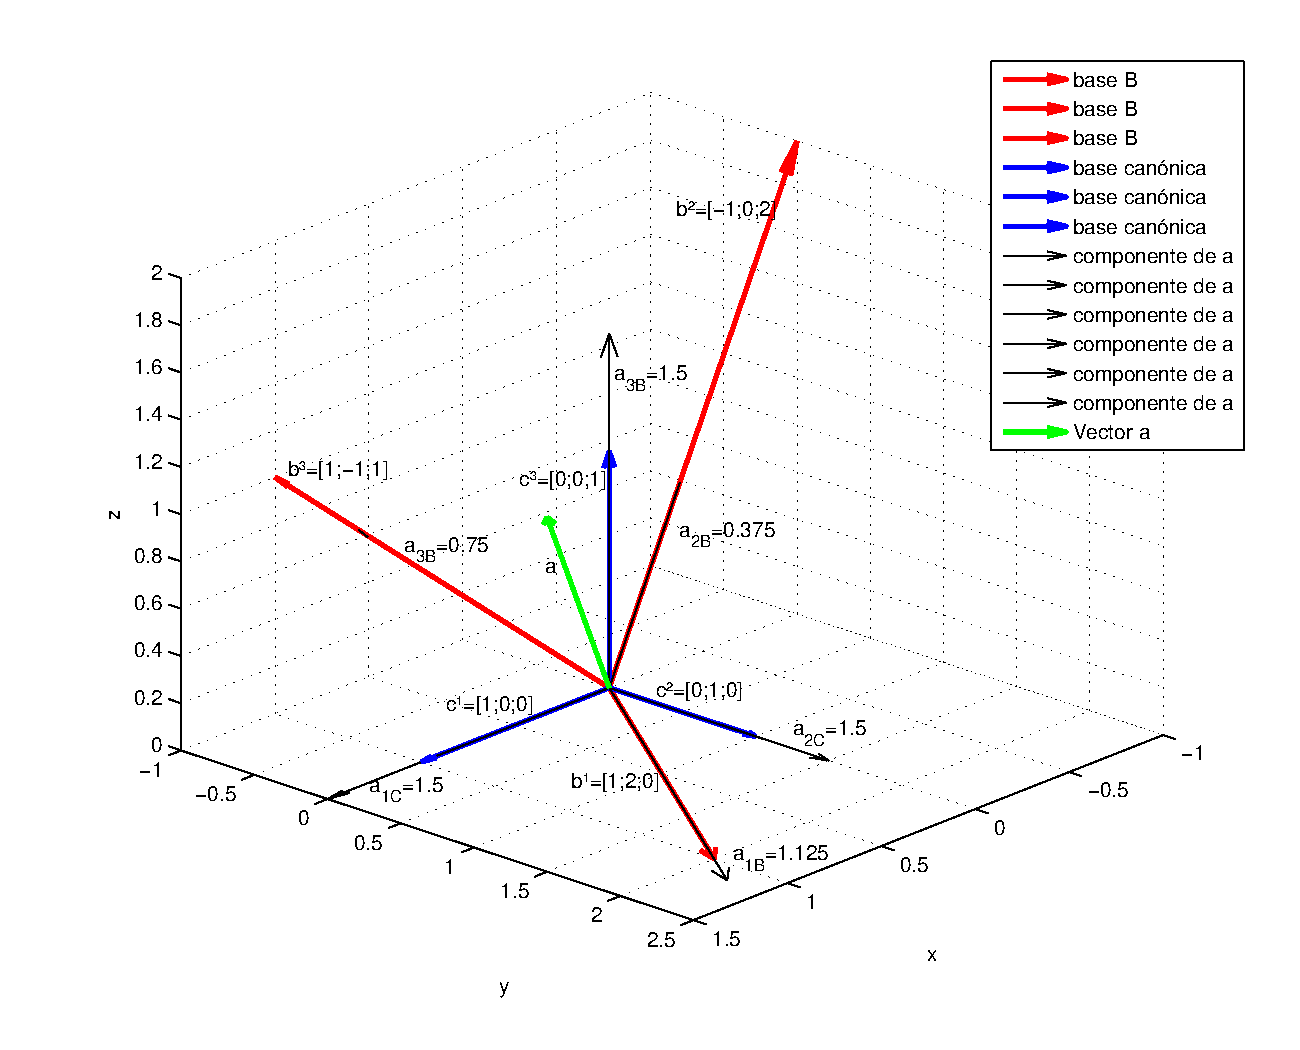
\includegraphics[width=15cm]{base1.eps}
\bicaption{Representación gráfica del vector $a$, en la base canónica $\mathcal{C}$ y en la base $\mathcal{B}$.}{Graphic representation of vector $a$, in the canonical basis $\mathcal{C}$ and in $\mathcal{B}$ basis.}
\label{fig:base1}
\end{figure}

\begin{equation*}
\mathcal{B}=\left\lbrace b^1=\begin{pmatrix}
b_{11}\\
b_{21}\\
b_{31}\\
\vdots \\
b_{n1}
\end{pmatrix},b^2=\begin{pmatrix}
b_{12}\\
b_{22}\\
b_{32}\\
\vdots \\
b_{n2}
\end{pmatrix},
\cdots
b^n=\begin{pmatrix}
b_{1n}\\
b_{2n}\\
\vdots \\
b_{(n-1)n}\\
b_{nn}
\end{pmatrix} \right\rbrace \rightarrow
B=\begin{pmatrix}
b_{11}&b_{12}& \cdots & b_{1n}\\
b_{21}&b_{22}& \cdots & b_{2n}\\
b_{31}&b_{32}& \cdots & \vdots \\
\vdots & \vdots & \cdots &  b_{(n-1)n}\\
b_{n1}&b_{n2}& \cdots & b_{nn}\\
\end{pmatrix}
\end{equation*}
\begin{paracol}{2}
Supongamos que tenemos un vector $a$ cuyas componentes en la base $\mathcal{B}$ son,
\switchcolumn
Supose now that we vector $a$ has the following components ins basis $\mathcal{B}$,
\end{paracol}

\begin{equation*}
a^{\mathcal{B}}=\begin{pmatrix}
a_1^{\mathcal{B}}\\
a_2^{\mathcal{B}}\\
\vdots \\
a_n^{\mathcal{B}}
\end{pmatrix}
\end{equation*}

\begin{paracol}{2}
Para obtener las componentes en la base canónica, basta entonces multiplicar la matriz $B$, por el vector $a^{\mathcal{B}}$. Así en el ejemplo que acabamos de ver,
\switchcolumn
we can obtain the componets on the canonical base just multiplying matrix $B$ for vector $a^{\mathcal{B}}$. So in the example we just have seen,
\end{paracol}

\begin{equation*}
a=B\cdot a^{\mathcal{B}} \rightarrow a=\begin{pmatrix}
1& -1& 1\\
2& 0& -1\\
0& 2& 1
\end{pmatrix}\cdot \begin{pmatrix}
1.125\\
0.375\\
0.75
\end{pmatrix}
= \begin{pmatrix}
1.5\\
1.5\\
1.5
\end{pmatrix}
\end{equation*}

\begin{paracol}{2}
Por último, podemos combinar el producto de matrices y la matriz inversa, para obtener las componentes de un vector en una base cualquiera a partir de sus componentes en otra base. Supongamos que tenemos dos bases $\mathcal{B}_1$ y $\mathcal{B}_2$ y un vector $a$. Podemos obtener las componentes de $a$ en la base canónica, a partir de las componentes en la base $\mathcal{B}_1$ como, $a=B_1\cdot a^{\mathcal{B}_1}$ y a partir de sus componentes en la base $\mathcal{B}_2$ como $a=B_2\cdot a^{\mathcal{B}_2}$. Haciendo uso de la matriz inversa,
\switchcolumn
Eventually, we can combine the matrix product and the inverse matrix to obtain the vector components in any basis whatsoever, knowing the vector components is other arbitrary basis. Suppose we have two bases $\mathcal{B}_1$ and $\mathcal{B}_2$ and a vector $a$. We can get the components of $a$ in the canonical basis from its components on basis $\mathcal{B}_1$ as, $a=B_1\cdot a^{\mathcal{B}_1}$  and from basis $\mathcal{B}_2$ as $a=B_2\cdot a^{\mathcal{B}_2}$.
Using the inverse matrix we obtain,
\end{paracol}

\begin{align*}
a&=B_1\cdot a^{\mathcal{B}_1} \Rightarrow a^{\mathcal{B}_1}=B_1^{-1} \cdot a \\
 a&=B_2\cdot a^{\mathcal{B}_2} \Rightarrow a^{\mathcal{B}_2}=B_2^{-1} \cdot a
\end{align*},

\begin{paracol}{2}
y sustituyendo obtenemos,
\switchcolumn
and, after replace, we obtain,
\end{paracol}

\begin{align*}
a^{\mathcal{B}_1}&=B_1^{-1}\cdot B_2 \cdot a^{\mathcal{B}_2}\\
a^{\mathcal{B}_2}&=B_2^{-1} \cdot B_1\cdot a^{\mathcal{B}_1} 
\end{align*}

\begin{paracol}{2}
El siguiente código permite cambiar de base un vector y, si el vector pertenece a $\mathbb{R}^3$, representa gráficamente tanto el vector como las bases antigua y nueva.
\switchcolumn
The following code allows us to change a vector from one basis to aanother. Besides, if the vector is in $\mathbb{R}^3$, the program represents the vector and the old a  the new bases.
\end{paracol}
\inputminted[
frame=lines,
framesep=2mm,
baselinestretch=1.2,
%bgcolor=LightGray,
label=cambio\_vb.py,
fontsize=\footnotesize,
linenos
]{python}{./codigos/Algebra/codigo_abierto/cambio_vb.py}

\begin{paracol}{2}
\paragraph{Operadores lineales.} A partir de los visto en las secciones anteriores, sabemos que el producto de una matriz de $A$ de orden $n\times n$  multiplicada por un vector $b$ de dimension $n$ da como resultado un nuevo vector $c=A\cdot b$  de dimensión $n$. Podemos considerar cada matriz $n\times n$ como un \emph{operador lineal}, que transforma unos vectores en otros.  Decimos que se trata de un operador lineal porque las componentes del vector resultante, están relacionadas linealmente con las del vector original, por ejemplo para $n=3$,
\switchcolumn
\paragraph{Linear operators.} In previous sections we sow that the product of a matrix $A$ of dimensions $n\times n$ by a vector $b$ of dimension $n$ cast a new vector $c$ of dimension $n$ as a result. We could consider every matrix $n\times n$ as a \emph{linear operator}, which transforms one vector into another. We define it as a linear operator because the components of the resulting vector are linearly related with the components of the operator (the original vector before the transformation). For example, in $n=3$,   

\end{paracol}

\begin{equation*}
\begin{pmatrix}
y_1\\
y_2\\
y_3
\end{pmatrix}=\begin{pmatrix}
a_{11}& a_{12}& a_{13}\\
a_{21}& a_{22}& a_{23}\\
a_{31}& a_{32}& a_{33}
\end{pmatrix} \cdot
\begin{pmatrix}
x_1\\
x_2\\
x_3
\end{pmatrix} \rightarrow \begin{matrix}
y_1=a_{11}x_1+a_{12}x_2+a_{13}x_3\\
y_2=a_{21}x_1+a_{22}x_2 +a_{23}x_3\\
y_3=a_{31}x_1+a_{32}x_2+a_{33}x_3
\end{matrix} 
\end{equation*}

\begin{paracol}{2}
Entre los operadores lineales, es posible destacar aquellos que producen transformaciones geométricas sencillas. Veamos algunos ejemplos para vectores bidimensionales,

1. Dilatación: aumenta el módulo de un vector en un factor $\alpha>1$. Contracción: disminuye el módulo de un vector en un factor $0<\alpha<1$. En ambos casos, se conserva la dirección y el sentido del vector original.
\switchcolumn
Some linear operator are particular interesting because they generate simple geometrical transformations. Let's see some examples for bi-dimensional vectors:

1. Dilation: Spans the module of a vector in a factor $\alpha>1$. Contraction: diminishes the module of a vector in a factor $0<\alpha<1$. In both cases, the direction and sense of the original vector is preserved.
\end{paracol} 
\begin{equation*}
R=\begin{pmatrix}
\alpha& 0\\
0& \alpha
\end{pmatrix} \rightarrow R\cdot a = \begin{pmatrix}
\alpha& 0\\
0& \alpha
\end{pmatrix} \cdot \begin{pmatrix}
a_1\\
a_2
\end{pmatrix}= \begin{pmatrix}
\alpha \cdot a_1\\
\alpha \cdot a_2
\end{pmatrix}
\end{equation*}
\begin{paracol}{2}
2. Reflexión de un vector respecto al eje x, conservando su módulo,
\switchcolumn
2. Reflection of a vector with respect to the x-axis, preserving its norm,
\end{paracol}
\begin{equation*}
R_x=\begin{pmatrix}
1& 0\\
0& -1
\end{pmatrix} \rightarrow R_x\cdot a = \begin{pmatrix}
1& 0\\
0& -1
\end{pmatrix} \cdot \begin{pmatrix}
a_1\\
a_2
\end{pmatrix}= \begin{pmatrix}
a_1\\
-a_2
\end{pmatrix}
\end{equation*}
\begin{paracol}{2}
3. Reflexión de un vector respecto al eje y, conservando su módulo,
\switchcolumn
3. reflection of a vector with respect to the y-axis, preserving its norm, 
\end{paracol}
\begin{equation*}
R_y=\begin{pmatrix}
-1& 0\\
0& 1
\end{pmatrix} \rightarrow R_y\cdot a = \begin{pmatrix}
-1& 0\\
0& 1
\end{pmatrix} \cdot \begin{pmatrix}
a_1\\
a_2
\end{pmatrix}= \begin{pmatrix}
-a_1\\
a_2
\end{pmatrix}
\end{equation*}
\begin{paracol}{2}
4. Reflexión respecto al origen: Invierte el sentido de un vector, conservando su módulo y dirección,
\switchcolumn

4. reflection with respect to the origin: Invert the sense of the vector, preserving its norm and direction. 
\end{paracol}
\begin{equation*}
R=\begin{pmatrix}
-1& 0\\
0& -1
\end{pmatrix} \rightarrow R\cdot a = \begin{pmatrix}
-1& 0\\
0& -1
\end{pmatrix} \cdot \begin{pmatrix}
a_1\\
a_2
\end{pmatrix}= \begin{pmatrix}
-a_1\\
-a_2
\end{pmatrix}
\end{equation*}
\begin{paracol}{2}
Sería equivalente a aplicar una reflexión respecto al eje x y luego respecto al eje y o viceversa,
\switchcolumn
It is equivalent to apply a refletion on x-axis and then a reflection on y-axis or vice versa,
\end{paracol}
$R=R_x\cdot R_y= R_y\cdot R_x$.
\begin{paracol}{2}
 5. Rotación en torno al origen un ángulo $\theta$,
 \switchcolumn
 5. Rotation an angle $\theta$ around the origin,
\end{paracol}
\begin{equation*}
R_{\theta}=\begin{pmatrix}
cos(\theta)& -sin(\theta)\\
sin(\theta)& cos(\theta)
\end{pmatrix} \rightarrow R_{\theta}\cdot a = \begin{pmatrix}
cos(\theta)& -sin(\theta)\\
sin(\theta)& cos(\theta)
\end{pmatrix} \cdot \begin{pmatrix}
a_1\\
a_2
\end{pmatrix}= \begin{pmatrix}
a_1cos(\theta)-a_2sin(\theta)\\
a_1sin(\theta)+a_2cos(\theta)
\end{pmatrix}
\end{equation*}


La figura \ref{fig:ltrans} muestra los vectores resultantes de aplicar las transformaciones lineales que acabamos de describir al vector,  $ a=\bigl( \begin{smallmatrix}
1\\
2
\end{smallmatrix} \bigr)$,

\begin{figure}[h]
\centering
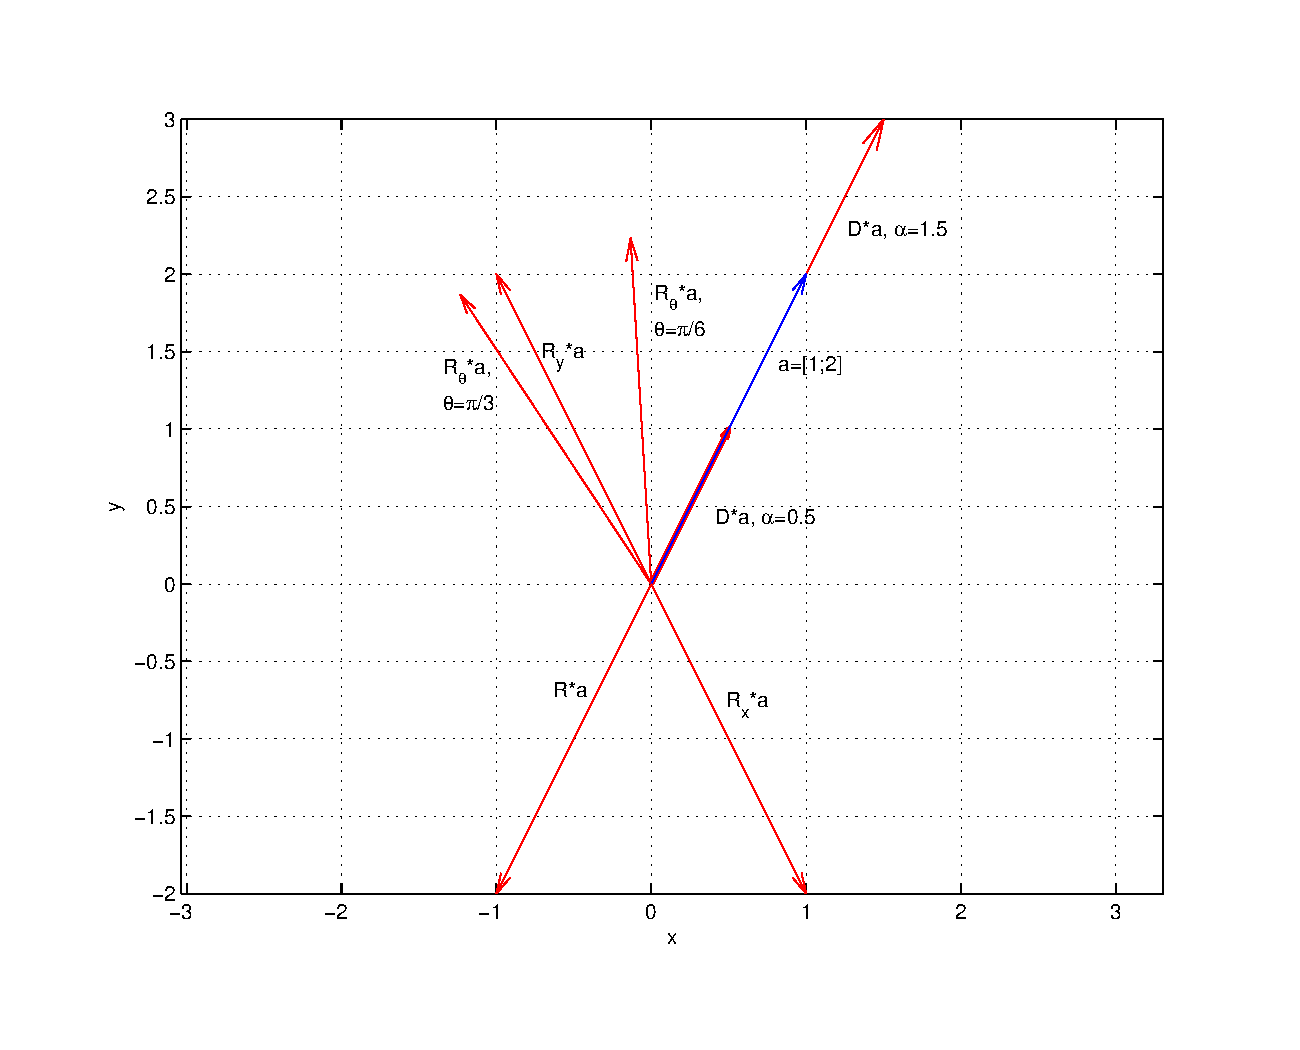
\includegraphics[width=12cm]{ltrans.eps}
\bicaption{Transformaciones lineales del vector $a=[1,2]$. $D$, dilatación/contracción en un factor $1.5$/$0.5$. $R_x$, reflexión respecto al eje x. $R_y$, reflexión respecto al eje y. $R_{\theta}$ rotaciones respecto al origen para ángulos $\theta=\pi /6$ y $\theta=\pi /3$}{Linear transformation of vector $=[1,1]$. $D$, factor $1.5$/$0.5$ dilation/contraction. $R_y$ reflection on y-axis. $R_{\theta}$ $\theta=\pi /6$ and $\theta=\pi /3$ angles rotations around the origin.}
\label{fig:ltrans}
\end{figure}

\begin{paracol}{2}
\paragraph{Norma de una matriz.} La norma de una matriz se puede definir a partir del efecto que produce al actuar, como un operador lineal, sobre un vector. En este caso, se les llama normas \emph{inducidas}. Para una matriz $A$ de orden $m\times n$, $y_{(m)}=A_{(m\times n)}x_{(n)}$, La norma inducida de $A$ se define en función de las normas de los vectores $x$ de su dominio y de las normas de los vectores $y$ de su rango como,
\switchcolumn
\paragraph{Matrix norm.} A matrix norm can be defined from the effect of the matrix when operates  on a vector as a linear operator. In this case, we call these norms \emph{induced} norms. For a matrix $A$ of dimensions $m\times n$, $y(m) =A_{m\times n}x_{(n)}$. The induced norm of $A$ is defined using the norms of the vectors $x$ of its domain and the norms of the vectors $y$ of its range, according to the following expression,   
\end{paracol}
\begin{equation*}
\Vert A \Vert =\max_{x \neq 0} \frac{\Vert y \Vert}{\Vert x \Vert}=\max_{x \neq 0} \frac{\Vert Ax \Vert}{\Vert x \Vert}
\end{equation*}

\begin{paracol}{2}
Se puede interpretar como el factor máximo con que el que la matriz $A$ puede \emph{alargar} un vector cualquiera. Es posible definir la norma inducida en función de los vectores unitarios del dominio,
\switchcolumn
It can be interpreted as the maximum factor a matrix $A$ can \emph{enlarge} any vector. Some times the induced norm is defined using the unitary vector of its domain,

\end{paracol}
\begin{equation*}
\Vert A \Vert =\max_{x \neq 0} \frac{\Vert Ax \Vert}{\Vert x \Vert}= \max_{x \neq 0} \left\Vert A\frac{x}{\Vert x \Vert} \right\Vert= \max_{\Vert x \Vert =1}\Vert Ax \Vert
\end{equation*}

\begin{paracol}{2}
Junto a la norma inducida que acabamos de ver, se definen las siguientes normas,

1. Norma $1$: Se suman los elementos de cada columna de la matriz, y se toma como norma el valor máximo de dichas sumas,
\switchcolumn
Besides the induced norm already described, it is possible to define the following norms,

1. Norm $1$: we add the entries of each column up and then take the maximun value of these sums as a norm
\end{paracol}
\begin{equation*}
\Vert A_{m,n} \Vert _{1} = \max_j \sum_{i=1}^m a_{ij}
\end{equation*}
\begin{paracol}{2}
2. Norma $\infty$: Se suman los elementos de cada fila y se toma como norma $\infty$ el valor máximo de dichas sumas.
\switchcolumn
2. Norm $\infty$: We add the entries of each row up and then take the maximum value of these sums as the $\infty$ norm.
\end{paracol}
\begin{equation*}
\Vert A_{m,n} \Vert _{\infty} = \max_i \sum_{j=1}^m a_{ij}
\end{equation*}
\begin{paracol}{2}
3. Norma 2: Se define como el mayor de los valores singulares de una matriz. (Ver sección \ref{sec:SVD}).

\switchcolumn
3. Norm $2$:it si defined as the largest of the matrix singular values. (See section \ref{sec:SVD}). 
\end{paracol}

\begin{equation*}
\Vert A_{m,n} \Vert _2 = \sigma_{1}
\end{equation*}
\begin{paracol}{2}
4. Norma de Frobenius. Se define como la raíz cuadrada de la suma de los cuadrados de todos los elementos de la matriz,

\switchcolumn
4.Frobenius' norm. It is defined as the square root of the sum of the squared values of the matrix entries, 
\end{paracol}
\begin{equation*}
\Vert A_{m,n} \Vert _F =\sqrt{\sum_{i=1}^m \sum_{j=1}^m a_{ij}^2}
\end{equation*}
\begin{paracol}{2}
Que también puede expresarse de forma mas directa como,
\switchcolumn
That can be also expressed in a more straightforward way as,
\end{paracol}
\begin{equation*}
\Vert A_{m,n} \Vert _F =\sqrt{tr(A^T\cdot A)}
\end{equation*}
\begin{paracol}{2}
En Numpy, es posible calcular las distintas normas de una matriz, de modo análogo a como se calculan para el caso de vectores,  mediante el comando \texttt{norm(A,p)}. Donde \texttt{A}, es ahora un a matriz y \texttt{p} especifica el tipo de norma que se quiere calcular. En el caso de una matriz, el parámetro \texttt{p} solo puede tomar los valores, \texttt{1} (norma 1), \texttt{2} (norma 2), \texttt{inf} (norma $\infty$), y \mintinline{python}{'fro'} (norma de frobenius). Esta última es la norma por defecto, y es la que se obtiene si se no se define el tipo de norma. El siguiente ejemplo muestra el cálculo de las normas 1, 2, $\infty$ y de Frobenius de la misma matriz.
\switchcolumn
In Numpy is possible to calculate the different matrix norms, similarly to how we calculate the norm of a vector, using the command \mintinline{python}{norm(A,p)}. Where \mintinline{python}{A} is now a matrix and \mintinline{python}{p} specifies the kind of norm we can calculate. In the case of a matrix, parameter \mintinline{python}{p} can take only the values, \mintinline{python}{1} (norm 1), \mintinline{python}{2} (norm 2), \mintinline{python}{inf}, (norm $\infty$), and \mintinline{python}{'fro'} (frobenius' norm). This last is the norm by default and, thus, if the norm Numpy calculates if parameter \mintinline{python}{p} is omitted. The following example shows the calculations of norms 1, 2, $\infty$, and Frobenius for the same matrix.  
\end{paracol}
\begin{center}
    \begin{minipage}{0.5\textwidth}
    \begin{minted}{python}
In [11]: A = np.array([[1,-1,3],[2,0,-2],[3,1,2]])

In [12]: A
Out[12]: 
array([[ 1, -1,  3],
       [ 2,  0, -2],
       [ 3,  1,  2]])

In [13]: np.linalg.norm(A)
Out[13]: 5.744562646538029

In [14]: np.linalg.norm(A,'fro')
Out[14]: 5.744562646538029

In [15]: np.linalg.norm(A,1)
Out[15]: 7.0

In [17]: np.linalg.norm(A,inf)
Out[17]: 6.0

In [18]: np.linalg.norm(A,2)
Out[18]: 4.552861506620628
\end{minted}
\end{minipage}
\end{center}

\begin{paracol}{2}
\paragraph{Formas cuadráticas.} Se define como forma cuadrática a la siguiente operación entre una matriz cuadrada $A$ de orden $n \times n$ y un vector $x$ de dimensión $n$,
\switchcolumn
\paragraph{Quadratic forms.} We define the following operation between a square matrix $A$ of dimensions $n\times n$ an a vector $x$ as a quadratic form,
\end{paracol}
\begin{equation*}
\alpha=x^T\cdot A \cdot x, \ \alpha \in \mathbb{R}
\end{equation*}

\begin{paracol}{2}
El resultado es un escalar. Así por ejemplo,
\switchcolumn
The result is a scalar. For instance,
\end{paracol}

\begin{equation*}
A=\begin{pmatrix}
1& 2& -1\\
2& 0& 2\\
3& 2& -2
\end{pmatrix}, \ x=\begin{pmatrix}
1\\
2\\
3
\end{pmatrix} \rightarrow \begin{pmatrix}
1& 2& 3
\end{pmatrix} \cdot \begin{pmatrix}
1& 2& -1\\
2& 0& 2\\
3& 2& -2
\end{pmatrix} \cdot \begin{pmatrix}
1\\
2\\
3
\end{pmatrix}= 21
\end{equation*}
\begin{paracol}{2}
Para dimensión $n=2$,
\switchcolumn
In $n=2$ dimension,
\end{paracol}
\begin{equation*}
\alpha =\begin{pmatrix}
x_1& x_2
\end{pmatrix}\cdot \begin{pmatrix}
a_{11}& a_{12}\\
a_{21}& a_{22}
\end{pmatrix}\cdot \begin{pmatrix}
x_1\\
x_2
\end{pmatrix} \rightarrow x_3\equiv \alpha=a_{11}x_1^2+(a_{12}+a_{21})x_1x_2+a_{22}x_2^2
\end{equation*}

\begin{paracol}{2}
Lo que obtenemos, dependiendo de los signos de $a_{11}$ y $a_{12}$, es la ecuación de un paraboloide o un hiperboloide. En la figura \ref{fig:parabol} Se muestra un ejemplo,
\switchcolumn
Depending of the sign of $a_{11}$ y $a_{12}$ we obtain  a paraboloid or a hyperboloid  equation. Figure \ref{fig:parabol} shows an example.
\end{paracol}
\begin{figure}[h]
\centering
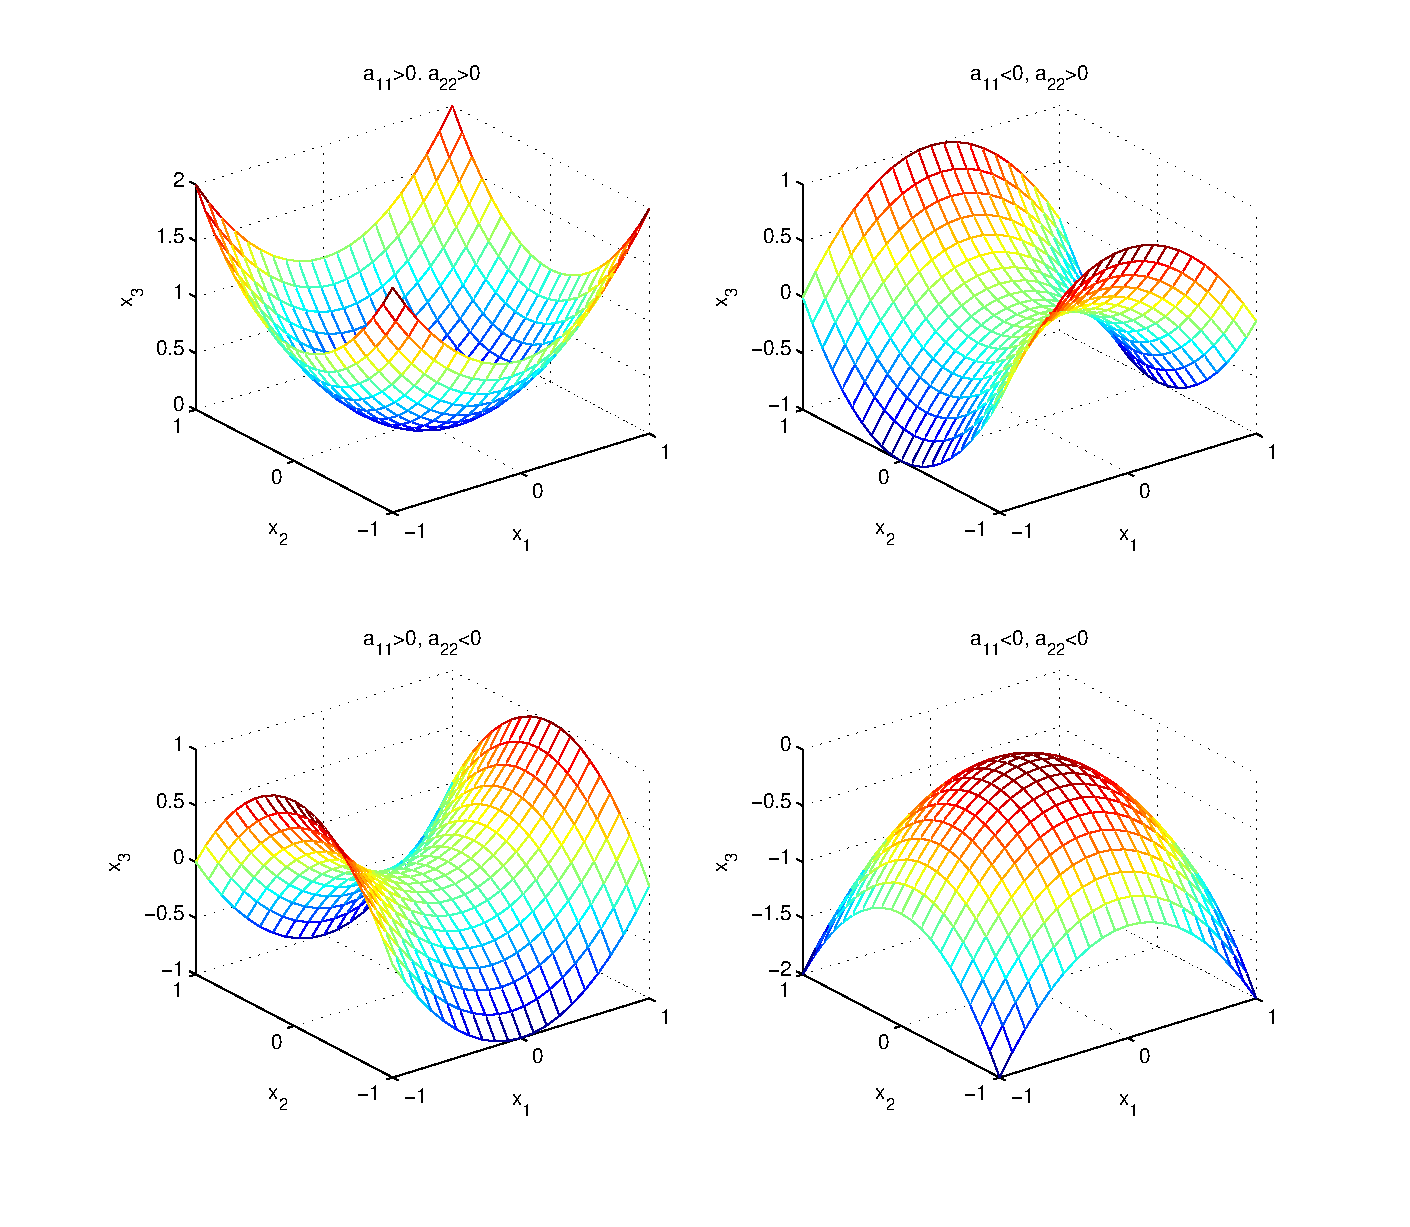
\includegraphics[width=14cm]{parabol.eps}
\bicaption{Formas cuadráticas asociadas a las cuatro matrices diagonales: $\vert a_{11}\vert=\vert a_{22}\vert=1$, $a_{12}=a_{21}=0$}{Quadratic forms obtained using the four diagonal matrices: $\vert a_{11}\vert=\vert a_{22}\vert=1$, $a_{12}=a_{21}=0$}
\label{fig:parabol}
\end{figure}
\begin{paracol}{2}
Veamos brevemente, algunas propiedades de las formas cuadráticas,

1. Una matriz $A$ de orden $ n\times n$ se dice que es definida positiva si da lugar a una forma cuadrática que es siempre mayor que cero para cualquier vector no nulo,

\switchcolumn
Briefly we will revise some quadratic forms properties, 

1. A matrix $A$ of dimensions $n\times n$ is positive definite is generates a quadratic form always greater than zero for any non-null vector.
\end{paracol}
\begin{equation*}
x^T \cdot A \cdot x > 0, \forall x \neq 0 
\end{equation*}
\begin{paracol}{2}
2. Una matriz \emph{simétrica} es definida positiva si todos sus \emph{valores propios} (ver sección \ref{sec:diag}) son positivos.

3. Una matriz no simétrica $A$ es definida positiva si su parte simétrica $A_s=(A+A^T)/2$ lo es.
\switchcolumn
2. A \emph{symmetric} matrix is positive definite if all its \emph{eigenvalues} (see section \ref{sec:diag}) are positive. 

3. A non-symmetric matrix $A$ is positive definite is it symmetric part $A_s=(A+A^T)/2$ be so. 
\end{paracol}
\begin{equation*}
x\cdot A_s\cdot >0, \forall x \neq 0 \Rightarrow x\cdot A\cdot >0, \forall x \neq 0
\end{equation*}

\begin{flalign*}
&&\rbrace \reversemathwitch*
\end{flalign*}

\begin{paracol}{2}
\section{Tipos de matrices empleados frecuentemente.}\label{tiposm}
Definimos a continuación algunos tipos de matrices frecuentemente empleados en álgebra, algunos ya han sido introducidos en secciones anteriores; los reunimos todos aquí para facilitar su consulta.

1 Matriz ortogonal: Una matriz $A_{n\times n}$ es ortogonal cuando su inversa coincide con su traspuesta.

\switchcolumn
\section{Kinds of matrices frequently used.}
We define next some kinds of matrices frequently used in algebra, some of then have been already introduced in previous sections; we put them together here for ease reference.

1 Ortogonal matrix: A matrix $A_{n\times n}$ is ortogonal whenever its inverse matrix is equal to its transpose.
 
\end{paracol}
\begin{equation*}
A^T=A^{-1}
\end{equation*}
\begin{paracol}{2}
ejemplo,
\end{paracol}

\begin{equation*}
A=\begin{pmatrix}
1/3& 2/3& 2/3\\
2/3& -2/3& 1/3\\
2/3& 1/3& -2/3\\
\end{pmatrix} \rightarrow A\cdot A^T =A^T\cdot A= \begin{pmatrix}
1& 0& 0\\
0& 1& 0\\
0& 0& 1
\end{pmatrix}
\end{equation*}
\begin{paracol}{2}
2. Matriz simétrica: Una matriz $A_{n\times n}$ es simétrica cuando es igual que su traspuesta,
\switchcolumn
2. Symmetric Matrix: A matrix $_{n\times n}$ is symmetric if it is equal to its transpose.
\end{paracol}
\begin{equation*}
A=A^T \rightarrow a_{ij}=a_{ji}
\end{equation*}
\begin{paracol}{2}
ejemplo,
\end{paracol}
\begin{equation*}
A=\begin{pmatrix}
1& -2& 3\\
-2& 4& 0\\
3& 0& -5
\end{pmatrix}
\end{equation*}
\begin{paracol}{2}
3. Matriz Diagonal: Una matriz $A$  es diagonal si solo son distintos de ceros los elementos de su diagonal principal,
\switchcolumn
3. Diagonal matrix: A matrix $A$ is diagonal is only the entries of its main diagonal are different from zero.
\end{paracol}

\begin{equation*}
\begin{pmatrix}
a_{11}& 0& \cdots & 0\\
0& a_{22}& \cdots & 0\\
\vdots & \vdots & \ddots & 0\\
0& 0& \cdots & a_{nn}
\end{pmatrix} \rightarrow
a_{ij}=0,\ \forall i\neq j
\end{equation*}

\begin{paracol}{2}
4. Matriz triangular superior: Una matriz cuadrada es triangular superior cuando todos los elementos situados por debajo de la diagonal son cero. Es estrictamente diagonal superior si además los elementos de la diagonal también son cero,
\switchcolumn
4. Upper triangular matrix: a square matrix is upper triangular when every entry below its main diagonal is zero, and if it is strictly upper triangular in all the diagonal entries are also zero.   
\end{paracol}
\begin{align*}
TRS& \rightarrow a_{ij} = 0, \ \forall i\geq j \\
ETRS& \rightarrow a_{ij} = 0, \ \forall i > j 
\end{align*}
\begin{paracol}{2}
ejemplos,
\end{paracol}

\begin{align*}
TRS&=\begin{pmatrix}
1 & 3 & 7\\
0 & 2 & -1\\
0 & 0 & 4
\end{pmatrix}\\
ETRS&=\begin{pmatrix}
0 & 3 & 7\\
0 & 0 & -1\\
0 & 0 & 0
\end{pmatrix}\\
\end{align*}
\begin{paracol}{2}
5. Matriz triangular inferior: Una matriz es triangular inferior si todos los elementos pro encima de su diagonal son cero. Es estrictamente triangular inferior si además los elementos de su diagonal son también cero,
\switchcolumn
5. Lower triangular matrix: A square matrix is lower triangular when every entry above its main diagonal are zero, and it si strictly lower triangular if all the diagonal entries are also zero. 
\end{paracol}
\begin{align*}
TRI& \rightarrow a_{ij} = 0, \ \forall i\leq j \\
ETRI& \rightarrow a_{ij} = 0, \ \forall i < j 
\end{align*}
\begin{paracol}{2}
ejemplos,
\end{paracol}

\begin{align*}
TRI&=\begin{pmatrix}
1 & 0 & 0\\
3 & 2 & 0\\
7 & -1 & 4
\end{pmatrix}\\
ETRI&=\begin{pmatrix}
0 & 0 & 0\\
3 & 0 & 0\\
7 & -1 & 0
\end{pmatrix}\\
\end{align*}
\begin{paracol}{2}
6. Matriz definida Positiva. Una matriz $A_{n \times n}$ es definida positiva si dado un vector $x$ no nulo cumple,
\switchcolumn
6. Positive definite matrix: A matrix $A_{n\times n} $ is positive definite is taking a non-null vector $x$ satisfy,
\end{paracol}
\begin{equation*}
x^T\cdot A \cdot x > 0, \ \forall x\neq 0,
\end{equation*}
\begin{paracol}{2}
si,
\switchcolumn
if,
\end{paracol}
\begin{equation*}
x^T\cdot A \cdot x \geq 0, \ \forall x\neq 0,
\end{equation*}
\begin{paracol}{2}
entonces la matriz $A$ es semidefinida positiva.

7. Una matriz es (strictamente) diagonal dominante si cada uno de los elementos de la diagonal en valor absoluto es ()mayor) mayor o igual que la suma de los valores absolutos de los elementos de la fila a la  que pertenece.

\switchcolumn
then matrix $A$ is positive semi-definite.

7. A matrix is (strictly) diagonally dominant if, for every row of the matrix, the magnitude of the diagonal entry in a row is (greater) greater than or equal to the sum of the magnitudes of all the other (off-diagonal) entries in that row.
\end{paracol}

\begin{equation*}
\lvert a_{ii} \rvert > \sum_{j\neq i} \lvert a_{ij} \rvert, \ \forall i
\end{equation*}
\begin{paracol}{2}
ejemplo,
\end{paracol}
\begin{equation*}
A=\begin{pmatrix}
10& 2 & 3\\
2& -5 & 1\\
4& -2 & 8
\end{pmatrix}\rightarrow \left\{ \begin{aligned}
10& > 2+3\\
5&> 2+1\\
8& > 4+2
\end{aligned} \right. 
\end{equation*}

\begin{paracol}{2}
\section{Factorización de matrices}\label{sec:fact}
La factorización de matrices, consiste en la descomposición de una matriz en el producto de dos o más matrices. Las matrices resultantes de la factorización se eligen de modo que simplifiquen, o hagan más robustas numéricamente determinadas operaciones matriciales: Cálculos de determinantes, inversas, etc. A continuación se describen las más comunes.

\subsection{Factorization LU}\label{sec:LU}
Consiste en factorizar una matriz como el producto de una matriz triangular inferior $L$ por una  matriz triangular superior $U$, $A=L\cdot U$. Por ejemplo,
\switchcolumn
\section{Matrix factorization.}
Factorizing a matrix consists on divide it into the product of two or more matrices. We choose the resulting factor matrices so that they simplify or make certain matrix operations more robust. For instance: matrix determinant calculation, obtaining inverse matrix , etc. Next, we will describe most common matrix factorizations.

\subsection{LU factorization.}
We factorize a matrix into the product of a lower triangular matrix $L$ by an upper triangular one $U$., $A=L\cdot U$. For instance, 

\end{paracol}
\begin{equation*}
\begin{pmatrix}
3& 4& 2\\
2& 0& 1\\
3& 2& 1
\end{pmatrix} = \begin{pmatrix}
1& 0& 0\\
^2/_3 & 1& 0\\
1& ^3/_4& 1
\end{pmatrix}\cdot \begin{pmatrix}
3& 4& 2\\
0& ^{-8}/_3& ^{-1}/_3\\
0& 0& ^{-3}/_4
\end{pmatrix}
\end{equation*}
\begin{paracol}{2}
Una aplicación inmediata, es el calculo del determinante. Puesto que el determinante de una matriz triangular, es directamente el producto de los elementos de la diagonal.

En el ejemplo anterior,
\switchcolumn
 A straightforward application is determinant calculation. Recall that a triangular matrix determinant is the product of their diagonal entries.
 
 So, from the previous example we obtain,
\end{paracol}
\begin{equation*}
\vert A \vert = 6 \equiv \vert L \vert\cdot\vert U\vert =1 \cdot 1 \cdot 1 \cdot 3 \cdot (-\frac{8}{3})\cdot (-\frac{3}{4})=6    
\end{equation*}

\begin{paracol}{2}
Describir un método para realizar la factorización LU de una matriz, queda fuera de los objetivos de estos apuntes. Sin embargo sí que utilizaremos el comando \mintinline{python}{lu} incluido en una librería de Python llamada Scipy para obtener directamente el resultado de una factorización LU. Es una librería parecida a Numpy y que, al igual que esta última contiene un gran numero de funciones matemáticas. De hecho Numpy y Scipy solapan un poco y hay determinadas funciones que pueden encontrarse en ambas librerías. El comando pertenece a un submodulo de Scipy llamado \mintinline{python}{linalg}. Admite como variable de entrada una matriz cuadrada $A$ y nos devuelve como salida una matriz de permutación $P$, de la que hablaremos enseguida, y una matriz triangular inferior $L$ y otra triangular superior $U$ de modo que se cumple que $A =PLU$.

A veces obtener la factorización LU directa de una matriz, pude llevar a cálculos que son numéricamente inestables afectando a la precisión del resultado. Una manera de paliar este efecto es permutar entre sí algunas de las filas de la matriz que se quiere factorizar y factorizar la versión permutada.

La permutación de las filas de una matriz $A$ de orden $n\times m$, se puede definir a partir del producto con las matrices de permutación de orden $n \times n$. Éstas se obtienen permutando directamente las filas de la matriz identidad $I_{n \times n}$. Si una matriz de permutación multiplica a otra matriz por la izquierda, permuta el orden de sus filas. Si la multiplica por la derecha. permuta el orden de sus columnas. Así por ejemplo, para matrices de orden $3 \times n$,

\switchcolumn
The description of method to calculate a matrix LU factorization is far beyond the scope of this notes. However, we do use the command \mintinline{python}{lu}, include in a Python library called Scipy, to compute the result of a LU factorization. Scipy is a library very much alike to Numpy and similarly to it, Scipy contains a large number of mathematical functions. In fact, Numpy and Scipy overlaps a little and you can find certain functions in both libraries. The \mintinline{python}{lu} command belongs to Scipy submodule called \mintinline{python}{linalg} and takes as input a square matrix $A$ of dimension $n\times n$, and returns as outputs a permutation matrix $P$ of dimension $n\times n$ we will describe later on, the lower triangula matrix $L$, and the upper triangular matrix $U$. The three output matrices satisfy $A=PLU$.

Sometimes obtaining directly the LU factorization of a matrix, leads to numerically instable calculations. This, in turn, affect the results precision. One way to overcome this problem is to permute some rows of the matrix we intend to factorize and then, to factorize the permuted version.

We can define the rows permutation of $A$ matrix of dimensions $n\times m$ multiplying the matrix by permutation matrices of dimensions $n\times n$. We obtain these last permuting the rows of the identity matrix $I_{n\times n}$.  When a permutation matrix multiplies another matrix by it left side, it permutes the order of the matrix rows. By contrast, if the permutation matrix multiplies another matrix by ts right, it permutes the order of the matrix columns. For instance, for matrix of dimensions $3\times n$, 

\end{paracol}
\begin{equation*}
I_{n \times n}=\begin{pmatrix}
1& 0& 0\\
0& 1& 0\\
0& 0& 1\\
\end{pmatrix} \rightarrow P_{1 \leftrightarrow 3}= \begin{pmatrix}
0& 0& 1\\
0& 1& 0\\
1& 0& 0\\
\end{pmatrix}
\end{equation*}
\begin{paracol}{2}
Si multiplicamos $P_{1 \leftrightarrow 3}$ con cualquier otra matriz $A$ de orden $3\times n$, El resultado es equivalente a intercambiar en la matriz $A$ la fila $1$ con la $3$. Por ejemplo,
\switchcolumn
If we multiply $P_{1\leftrightarrow 3}$ by any other matrix $A$ of dimensions $3\times n$, the result is equivalent to interchange row 1 and 3. For example, 
\end{paracol}
\begin{equation*}
P_{1\leftrightarrow 3}\cdot A=\begin{pmatrix}
0& 0& 1\\
0& 1& 0\\
1& 0& 0\\
\end{pmatrix} \cdot \begin{pmatrix}
1& 2& 5& 3\\
4& 2& 3& 0\\
3& 6& 2& 1
\end{pmatrix} = \begin{pmatrix}
3& 6& 2& 1\\
4& 2& 3& 0\\
1& 2& 5& 3
\end{pmatrix}= A_{1\leftrightarrow 3}
\end{equation*}

% Volvamos al cálculo de la factorización LU, pero ahora empleando la permutación de filas. Supongamos una matriz $A$ de orden $n\times n$

% El primer paso, es buscar el elemento mayor en valor absoluto de la primera columna en intercambia la primera fila de la matriz de $A$, con la fila que contiene dicho elemento. Si utilizamos la matriz de permutación adecuada, esto puede expresarse como,

% \begin{equation*}
% A \rightarrow P_1\cdot A
% \end{equation*}
% A continuación eliminamos los elementos de la primera fila situados por debajo de la diagonal,
% \begin{equation*}
% A \rightarrow P_1\cdot A \rightarrow \lambda_1 \cdot P_1 \cdot A
% \end{equation*}
% Volvemos a buscar el mayor elemento en valor absoluto para la segunda columna (Solo desde la diagonal hasta el ultimo elemento de la columna).  
% \begin{equation*}
% A \rightarrow P_1\cdot A \rightarrow \lambda_1 \cdot P_1 \cdot A \rightarrow  P_2 \cdot \lambda_1 \cdot P_1 \cdot A 
% \end{equation*}

% Eliminamos los elementos de la segunda fila situados por debajo de la diagonal,

% \begin{equation*}
% A \rightarrow P_1\cdot A \rightarrow \lambda_1 \cdot P_1 \cdot A \rightarrow  P_2 \cdot \lambda_1 \cdot P_1 \cdot A \rightarrow \lambda_2 \cdot  P_2 \cdot \lambda_1 \cdot P_1 \cdot A
% \end{equation*}

% Si seguimos todo el proceso hasta eliminar los elementos situados por debajo de la diagonal en la fila $n-1$, obtendremos la expresión de la matriz triangular superior $U$ resultante,

% \begin{equation*}
% \lambda_{n-1}P_{n-1}\lambda_{n-2}P_{n-2} \cdots  \lambda_2  P_2 \lambda_1  P_1 A = U
% \end{equation*}

% Aunque hemos obtenido $U$, necesitamos una manera de obtener $L$, ahora no es inmediato como en el caso de la factorización sin pivoteo, no basta con invertir las matrices $\lambda_i$ ya que tenemos por medio todas las matrices de permutación utilizadas. Para obtenerla realizaremos la siguiente transformación, 

% \begin{equation*}
% \lambda_{n-1}P_{n-1}\lambda_{n-2}P_{n-2} \cdots  \lambda_2  P_2 \lambda_1  P_1 A = \lambda_{n-1}'\lambda_{n-2}'\cdots \lambda_2'   \lambda_1' P_{n-1}P_{n-2} \cdots P_2  P_1 A
% \end{equation*}

% Donde las matrices $\lambda_i'$ pueden obtenerse a partir de las matrices $\lambda_i$ y de las matrices de permutación de la manera siguiente,

% \begin{align*}
% \lambda_{n-1}' &= \lambda_{n-1} \\
% \lambda_{n-2}' &= P_{n-1}\lambda_{n-2} P_{n-1} ^{-1}\\
% \lambda_{n-3}' &= P_{n-1}P_{n-2}\lambda_{n-3}P_{n-2}^{-1} P_{n-1}^{-1} \\
%  & \vdots \\
%  \lambda_{k\ \ }'  &= P_{n-1}P_{n-2}\cdots P_{k+1} \lambda_{k}P_{k+1}^{-1} \cdots P_{n-2}^{1} P_{n-1}^{-1} \\
%  & \vdots \\
% \lambda_{2\ \ }'  &= P_{n-1}P_{n-2}\cdots P_3 \lambda_{2}P_3^{-1} \cdots P_{n-2}^{1} P_{n-1}^{-1} \\
% \lambda_{1\ \ }'  &= P_{n-1}P_{n-2}\cdots P_3P_2 \lambda_{1}P_2^{-1}P_3^{-1} \cdots P_{n-2}^{1} P_{n-1}^{-1} \\
% \end{align*}


% Matemáticamente el cálculo de las matrices $\lambda_i'$ requiere calcular el producto de un gran número de matrices.  Sin embargo dicho cálculo es equivalente a permutar los elementos de $\lambda_i$ situados por debajo de la diagonal.   Así Por ejemplo para,

% \begin{equation*}
% \lambda_2=
% \begin{pmatrix}
% 1& 0& 0& 0\\
% 0& 1& 0& 0\\
% 0& 2& 1& 0\\
% 0& 3& 0& 1
% \end{pmatrix}, \ 
% P_3=
% \begin{pmatrix}
% 1& 0& 0& 0\\
% 0& 1& 0& 0\\
% 0& 0& 0& 1\\
% 0& 0& 1& 0
% \end{pmatrix}
% \end{equation*}

% \begin{equation*}
% \lambda_2'=P_3\cdot \lambda_2 P_3^{-1}
% \begin{pmatrix}
% 1& 0& 0& 0\\
% 0& 1& 0& 0\\
% 0& 0& 0& 1\\
% 0& 0& 1& 0
% \end{pmatrix}\cdot \begin{pmatrix}
% 1& 0& 0& 0\\
% 0& 1& 0& 0\\
% 0& 2& 1& 0\\
% 0& 3& 0& 1
% \end{pmatrix} \cdot \begin{pmatrix}
% 1& 0& 0& 0\\
% 0& 1& 0& 0\\
% 0& 0& 0& 1\\
% 0& 0& 1& 0
% \end{pmatrix} = \begin{pmatrix}
% 1& 0& 0& 0\\
% 0& 1& 0& 0\\
% 0& 3& 1& 0\\
% 0& 2& 0& 1
% \end{pmatrix}
% \end{equation*}

% Por último podemos representar el producto de todas las matrices de permutación como una sola matriz, $P_{n-1}P_{n-2} \cdots P_2  P_1=P$. (El producto de matrices de permutación entre sí, da como resultado una nueva matriz de permutación.

 
% De esta manera, la factorización LU con pivoteo de filas podríamos representarla como $P\cdot A=L\cdot U$,

% \begin{equation*}
% \overbrace{P_{n-1}P_{n-2} \cdots P_2  P_1}^{P}\cdot  A= \overbrace{\lambda_1'^{-1} \lambda_2'^{-2} \cdots \lambda_{n-2}'^{-1} \lambda_{n-1}'^{-1}}^{L}\cdot \overbrace{\lambda_{n-1}P_{n-1}\lambda_{n-2}P_{n-2} \cdots  \lambda_2  P_2 \lambda_1  P_1 A }^{U}   
% \end{equation*}
\begin{paracol}{2}
Volviendo a la factorización LU, vamos a ver como se calcularía para la siguiente matriz,	
\switchcolumn
Coming back to LU factorization, we are going to calculate it for the following matrix,
\end{paracol}
\begin{equation*}
A=\begin{pmatrix}
3& 4& 2&5\\
2& 0& 1& -2\\
3& 2& 1& 8\\
5& 2& 3& 2
\end{pmatrix} 
\end{equation*}

\begin{paracol}{2}
 Scipy, calcula siempre la factorización LU, permutando las filas para obtener un resultado lo mas preciso posible,
 \switchcolumn
 Scipy always use row permutation, when calculating an LU factorization, to obtain a result as accurate as possible,   
\end{paracol}

\begin{center}	
\begin{minipage}{0.7\textwidth}
\begin{minted}{python}
In [213]: A = np.array([[3,4,2,5],[2,0,1,-2],[3,2,1,8],[5,2,3,2]])

In [214]: A
Out[214]: 
array([[ 3,  4,  2,  5],
       [ 2,  0,  1, -2],
       [ 3,  2,  1,  8],
       [ 5,  2,  3,  2]])

In [215]: import scipy as sp

In [216]: [P,L,U] = sp.linalg.lu(A)

In [217]: P
Out[217]: 
array([[0., 1., 0., 0.],
       [0., 0., 0., 1.],
       [0., 0., 1., 0.],
       [1., 0., 0., 0.]])


In [218]: L
Out[218]: 
array([[ 1.        ,  0.        ,  0.        ,  0.        ],
       [ 0.6       ,  1.        ,  0.        ,  0.        ],
       [ 0.6       ,  0.28571429,  1.        ,  0.        ],
       [ 0.4       , -0.28571429,  0.16666667,  1.        ]])
\end{minted}
\end{minipage}
\end{center}

\begin{center}
\begin{minipage}{0.7\textwidth}
\begin{minted}{python}

In [219]: U
Out[219]: 
array([[ 5.        ,  2.        ,  3.        ,  2.        ],
       [ 0.        ,  2.8       ,  0.2       ,  3.8       ],
       [ 0.        ,  0.        , -0.85714286,  5.71428571],
       [ 0.        ,  0.        ,  0.        , -2.66666667]])

In [220]: P @ L @ U
Out[220]: 
array([[ 3.,  4.,  2.,  5.],
       [ 2.,  0.,  1., -2.],
       [ 3.,  2.,  1.,  8.],
       [ 5.,  2.,  3.,  2.]])
\end{minted}
\end{minipage}
\end{center}

\begin{paracol}{2}
\subsection{Factorización de Cholesky}\label{chol}
Dada una matriz cuadrada, simétrica y definida positiva, es siempre posible factorizarla como $A=L\cdot L^T$. Donde $L$ es una matriz triangular inferior,
\switchcolumn
\subsection{Cholesky factorisation}
Given a square simetric positive definite matrix, it always possible to factorize it as $A=L\cdot L^T$. Where $L$ is a lower triangular matrix.
\end{paracol}

\begin{equation*}
\begin{pmatrix}
a_{11}& a_{12}& \cdots & a_{1n}\\
a_{12}& a_{22}& \cdots & a_{2n}\\
\vdots & \vdots & \ddots & \vdots\\
a_{1n}& a_{2n}& \cdots & a_{nn}
\end{pmatrix}=\begin{pmatrix}
L_{11}& 0& \cdots & 0\\
L_{21}& L_{22}& \cdots & 0\\
\vdots & \vdots & \ddots & \vdots\\
L_{n1}& L_{n2}& \cdots & L_{nn}
\end{pmatrix} \cdot \begin{pmatrix}
L_{11}& L_{21}& \cdots & L_{n1}\\
0& L_{22}& \cdots & L_{n2}\\
\vdots & \vdots & \ddots & \vdots\\
0& 0& \cdots & L_{nn}
\end{pmatrix}
\end{equation*}
\begin{paracol}{2}
Numpy tiene una función, en el submódulo \mintinline{python}{linalg}, llamada \mintinline{python}{cholesky}, que permite obtener la factorización de Cholesky.
\switchcolumn
Numpy has a function, included in the \mintinline{python}{linalg} submodule, called \mintinline{python}{cholesky}, to calculate the cholesky factorization of a matrix.
\end{paracol}
\begin{center}
    \begin{minipage}{0.5\textwidth}
    \begin{minted}{python}
In [224]: B
Out[224]: 
array([[47, 28, 26, 45],
       [28, 24, 16, 40],
       [26, 16, 15, 22],
       [45, 40, 22, 97]])

In [225]: L = np.linalg.cholesky(B)

In [226]: L
Out[226]: 
array([[ 6.8556546 ,  0.        ,  0.        ,  0.        ],
       [ 4.08421976,  2.70539257,  0.        ,  0.        ],
       [ 3.79248978,  0.18874832,  0.76249285,  0.        ],
       [ 6.56392462,  4.87599823, -5.00195311,  2.2627417 ]])
    \end{minted}        
\end{minipage}
\end{center}

\begin{center}
	\begin{minipage}{0.5\textwidth}
		\begin{minted}{python}
In [227]: L @ L.T
Out[227]: 
array([[47., 28., 26., 45.],
       [28., 24., 16., 40.],
       [26., 16., 15., 22.],
       [45., 40., 22., 97.]])
    \end{minted}        
    \end{minipage}
\end{center}

\begin{paracol}{2}
Si la matriz no es definida positiva, la función \mintinline{python}{cholesky} da un mensaje de error.

\subsection{Diagonalización}\label{sec:diag}
\paragraph{Autovectores y autovalores.} Dada una matriz $A$ de orden $n\times n$, se define como autovector, o vector propio de dicha matriz al vector $x$ que cumple,
\switchcolumn
If the matrix is not definite posive, then function \mintinline{python}{cholesky} returns an error message.
\subsection{Diagonalisation}
\paragraph{Eigenvectors and eigenvalues.} We define an eigenvector or characteristic vector $x$ of the $n\times n$ matrix $A$ as, 
\end{paracol}
\begin{equation*}
A\cdot x =\lambda \cdot x, \  x\neq 0, \ \lambda \in \mathbb{C}
\end{equation*}
\begin{paracol}{2}
Es decir, el efecto de multiplicar la matriz $A$ por el vector $x$ es equivalente a multiplicar el vector $x$  por un número $\lambda$. Tanto $X$ como $\lambda$ pueden ser reales o complejos.

$\lambda$ recibe el nombre de autovalor, o valor propio de la matriz $A$ asociado al autovector $x$. Así por ejemplo,
\switchcolumn
Namely, the result of multiply matrx $A$ for its eigenvector $x$ is equal to multiply the number, $\lambda$ for the eigen vector. $x$ and $\lambda$ could be real or complex.

$\lambda$ is call de eigenvalue or characteristic values of the matrix $A$, associated to the eigenvector $x$. For example,`
\end{paracol}
\begin{equation*}
A= \begin{pmatrix}
-2& 0& 0\\
0& 2 & -1\\
0& 0& 3
\end{pmatrix}
\end{equation*}

\begin{paracol}{2}
tiene un autovalor $\lambda=3$ para el vector propio $x=[0,\  -3,\  3]^T$ ,
\switchcolumn
It has an eigenvalue $\lambda=3$ for the eigenvector $x=[0,\  -3,\  3]^T$ ,
\end{paracol}

\begin{equation*}
\begin{pmatrix}
-2& 0& 0\\
0& 2 & -1\\
0& 0& 3
\end{pmatrix}\cdot \begin{pmatrix}
0\\
-3\\
3
\end{pmatrix}=3\cdot \begin{pmatrix}
0\\
-3\\
3
\end{pmatrix}=\begin{pmatrix}
0\\
-9\\
9
\end{pmatrix}
\end{equation*}
\begin{paracol}{2}
El vector propio asociado a un valor propio no es único, si $x$ es un vector propio de una matriz $A$, asociado a un valor propio $\lambda$, Es trivial comprobar que cualquier vector de la forma $\alpha\cdot x, \ \alpha \in \mathbb{C}$ también es u vector propio asociado a $\lambda$,
\switchcolumn
There is not a single eigenvector associated to an eigenvalue, if $x$ is an eigenvector of a matrix $A$, associated to an eigenvalue $\lambda$, It is easy to check that any other vector that we build as $\alpha \cdot x, \ \alpha \in \mathbb{C}$ is also an eigenvector associated to $\lambda$, 
\end{paracol}
\begin{equation}
A\cdot x= \lambda x \Rightarrow A \cdot \alpha x = \lambda  \alpha x
\end{equation}
\begin{paracol}{2}
El conjunto de todos los autovalores de una matriz $A$ recibe el nombre de espectro de $A$ y se representa como $\Lambda(A)$.
Una descomposición en autovalores de una matriz $A$ se define como,
\switchcolumn
 we define the set of all eigenvalues of a matrix $A$ as the spectrum of $A$ and we represented it as $\Lambda(A)$. The eigendecomposition of a matrix $A$ is defined as,
\end{paracol}
\begin{equation*}
A=X\cdot D \cdot X^{-1}
\end{equation*}
\begin{paracol}{2}
Donde $D$ es una matriz diagonal formada por los autovalores de $A$. 
\switchcolumn
Where $D$ is a diagonal matrix built using the eigenvalues of $A$.
\end{paracol}
\begin{equation*}
\begin{pmatrix}
\lambda_1& 0 & \cdots & 0\\
0& \lambda_2& \cdots & 0\\
\vdots & \vdots& \cdots & 0\\
0& 0& \cdots & \lambda_n
\end{pmatrix}
\end{equation*}
\begin{paracol}{2}
Esta descomposición no siempre existe.  
\switchcolumn
The eigendescomposition does not always exist.  
\end{paracol}
\begin{flalign*}
&\mathwitch*_{i=0}^{\infty}\Xi_i(t)\lbrace &     
\end{flalign*}
\begin{paracol}{2}
En general, si dos matrices $A$ y $B$ cumplen,
\switchcolumn
In general, if two matrices $A$ and $B$ satisfy,
\end{paracol}
\begin{equation*}
A=X\cdot B \cdot X^{-1}
\end{equation*}
\begin{paracol}{2}
se dice de ellas que son similares. A la transformación que lleva a convertir $B$ en $A$ se le llama una transformación de semejanza. Una matriz es diagonalizable cuando admite una transformación de semejanza con una matriz diagonal de autovalores. 

Volviendo al ejemplo anterior podemos factorizar la matriz $A$ como,
\switchcolumn
Their a similar matrices. The transformation that convert $A$ into $B$ is denoted a similarity transformation. A matrix is diagonalisable when there is a similarity transformation that converts it in a diagonal matrix formed by its eigenvalues.

Coming back to the previous example we can factorise matrix $A$ as, 
\end{paracol}

\begin{equation*}
A= \begin{pmatrix}
-2& 0& 0\\
0& 2 & -1\\
0& 0& 3
\end{pmatrix}=\begin{pmatrix}
1& 0& 0\\
0& -1& -3\\
0& 0& 3
\end{pmatrix}\cdot \begin{pmatrix}
-2& 0& 0\\
0& 2& 0\\
0& 0& 3
\end{pmatrix} \cdot \begin{pmatrix}
1& 0& 0\\
0& -1& -1\\
0& 0& 1/3
\end{pmatrix}
\end{equation*}
\begin{paracol}{2}
Por tanto en este ejemplo, los autovalores de $A$ serían $\lambda_1=-2$, $\lambda_2=2$ y $\lambda_3=3$. Para estudiar la composición de la matriz $X$ Reescribimos la expresión de la relación de semejanza de la siguiente manera,
\switchcolumn
So, in this example the $A$ eigenvectors would be $\lambda_1=-2$, $\lambda_2=2$ and $\lambda_3=3$. To study the structure of matrix $X$, we rewrite the similarity relashionship as follows,
\end{paracol}

\begin{equation*}
 A=X \cdot D \cdot X^{-1}\rightarrow A\cdot X= X\cdot D
\end{equation*}
\begin{paracol}{2}
Si consideramos ahora cada columna de la matriz $X$ como un vector,
\switchcolumn
Now, we can consider each column of matrix $X$ as a vector,
\end{paracol}
\begin{equation*}
A\cdot X= X\cdot D \rightarrow A\cdot \left( x_1 | x_2 | \cdots | x_n \right)= \left( x_1 | x_2 | \cdots | x_n \right) \cdot\begin{pmatrix}
\lambda_1& 0 & \cdots & 0\\
0& \lambda_2& \cdots & 0\\
\vdots & \vdots& \cdots & 0\\
0& 0& \cdots & \lambda_n
\end{pmatrix}
\end{equation*}
\begin{paracol}{2}
Es fácil comprobar que si consideramos el producto de la matriz $A$, por cada una de las columnas de la matriz $X$ se cumple,
\switchcolumn
It is easy to check that the product of matrix $A$ by each column of matrix $X$ satisfy, 
\end{paracol}
\begin{align*}
A\cdot x_1 &=\lambda_1 \cdot x_1 \\
A\cdot x_2 &=\lambda_2 \cdot x_2 \\
\vdots \\
A\cdot x_n &=\lambda_n \cdot x_n \\
\end{align*}
\begin{paracol}{2}
Lo que nos lleva a que cada columna de la matriz $X$ tiene que ser un autovector de $A$ puesto que cumple,
\switchcolumn
But then, each column of matrix $x$ must be an eigenvector of $A$ because they satisfy,
\end{paracol}
\begin{equation*}
A\cdot x_i =\lambda_i \cdot x_i \\
\end{equation*}
\begin{paracol}{2}
En realidad, cada valor propio expande un subespacio $E_{\lambda}S$ de $\mathbf{C}^n$. Aplicar la matriz $A$, a un vector de $E_{\lambda}S$ es equivalente a multiplicar el vector por $\lambda$. Cada subespacio asociado a un autovalor recibe el nombre de autosubespacio o subespacio propio.

\paragraph{Polinomio característico.} El polinomio característico de una matriz $A$ de dimensión $n\times n$, se define como,

\switchcolumn
Actually, each eigenvalue expand a subspace $E_{\lambda}S$ of $\mathbf{C}^n$. To apply matrix $A$ to a vector in $E_{\lambda}S$  is identical to multiply the eigenvector by $\lambda$. Each subspace associated to an eigenvector is called an eigensubspace.
\paragraph{Characteristic polynomial.} The characteristic polynomial of a matrix $A$ with dimensions $n\times n$, is defined as, 
\end{paracol}
\begin{equation*}
P_A(z)=det(zI-A)
\end{equation*}
\begin{paracol}{2}
Donde $I$ es a matriz identidad de dimensión $n \times n$. Así por ejemplo para una matriz de dimensión $2\times 2$,
\switchcolumn
Where $I$ is the $n\times n$ identity matrix . For instance, for a matrix with dimensions $2\times 2$,
\end{paracol}
\begin{align*}
P_A(z)=&det\left(z\cdot \begin{pmatrix}
1& 0\\
0& 1
\end{pmatrix}- \begin{pmatrix}
a_{11}& a_{12}\\
a_{21}& a_{22}
\end{pmatrix} \right)=\left\vert \begin{matrix}
z-a_{11}& -a_{12}\\
-a_{21}& z-a_{22}
\end{matrix} \right\vert=\\
\\
=&(z-a_{11})\cdot(z-a_{22})-a_{12}\cdot a_{21}=z^2-(a_{11}+a_{22})\cdot z+a_{11}\cdot a_{22}-a_{12}\cdot a_{21}
\end{align*}
\begin{paracol}{2}
Los autovalores $\lambda$ de una matriz $A$ son las raíces del polinomio característico de la matriz $A$,
\switchcolumn
The eigenvalues $\lambda$ of matrix $A$ are the roots of the  characteristic polynomial of matrix $A$.
\end{paracol}
\begin{equation*}
p_A(\lambda)=0
\end{equation*}
\begin{paracol}{2}
Las raíces de un polinomio pueden ser simples o múltiples, es decir una misma raíz puede repetirse varias veces. Por tanto, los autovalores de una matriz, pueden también repetirse. Se llama multiplicidad algebraica de un autovalor al número de veces que se repite.

Además las raíces de un polinomio pueden ser reales o complejas. Para una matriz cuyos elementos son todos reales, si tiene autovalores complejos estos se dan siempre como pares de números complejos conjugados. Es decir si $\lambda =a+bi$ es un autovalor entonces $\lambda^*=a-bi$ también lo es.

Veamos algunos ejemplos:

La matriz,

\switchcolumn
The roots of a polynomial may be single of multiple that is the same root can be repeated several times. So, the autovalues of a matrix can also be repeated.

Besides, the roots of a polynomial may be real or complex. For a matrix with real elements, if it has complex eigenvalues their al always pairs complex conjugated numbers. That is, if $\lambda =a+bi$ is an eigenvalue then $\lambda^*=a-bi$ is also an eigenvalue.

Let's have a look to some examples:

The matrix, 
\end{paracol}
\begin{equation*}
A=\begin{pmatrix}
3& 2\\
-2& -2
\end{pmatrix}
\end{equation*}
\begin{paracol}{2}
Tiene como polinomio característico,
\switchcolumn
has characteristic polynomial, 
\end{paracol}
\begin{equation*}
P_A(z)=\left\vert\begin{matrix}
z-3& -2\\
2& z+2 
\end{matrix} \right\vert=z^2-z-2
\end{equation*}
\begin{paracol}{2}
Igualando el polinomio característico a cero y obteniendo las raíces de la ecuación de segundo grado resultante, obtenemos los autovalores de la matriz $A$,
\switchcolumn
If we equals the characteristic polynomial to zero and compute the roots of the resulting quadratic equation, we obtain the eigenvalues of matrix $A$
\end{paracol}
\begin{equation*}
\lambda^2-\lambda-2=0 \rightarrow \left\{ 
\begin{aligned}
\lambda_1&=2\\
\lambda_2&=-1
\end{aligned}
\right.
\end{equation*}
\begin{paracol}{2}
Un vector propio asociado a $\lambda_1=2$ sería $x_1=[2,\  -1]^T$,
\switchcolumn
An associated eigenvector to $\lambda_1=2$  would be $x_1=[2,\  -1]^T$,
\end{paracol}
\begin{equation*}
\begin{pmatrix}
3& 2\\
-2& -2
\end{pmatrix}\cdot \begin{pmatrix}
2\\
-1
\end{pmatrix}=2\cdot \begin{pmatrix}
2\\
-1
\end{pmatrix} =\begin{pmatrix}
4\\
-2
\end{pmatrix} 
\end{equation*}
\begin{paracol}{2}
y un vector propio asociado a $\lambda_2=-1$ sería $x_2=[1\ -2]^T$,
\switchcolumn
An an associated vector to $\lambda_2=-1$ would be $x_2=[1\ -2]^T$,
\end{paracol}
\begin{equation*}
\begin{pmatrix}
3& 2\\
-2& -2
\end{pmatrix}\cdot \begin{pmatrix}
1\\
-2
\end{pmatrix}=-1\cdot \begin{pmatrix}
1\\
-2
\end{pmatrix} =\begin{pmatrix}
-1\\
2
\end{pmatrix} 
\end{equation*}
\begin{paracol}{2}
La matriz,
\switchcolumn
the matrix,
\end{paracol}
\begin{equation*}
B=\begin{pmatrix}
4& -1\\
1& 2
\end{pmatrix}
\end{equation*}
\begin{paracol}{2}
tiene como polinomio característico,
\switchcolumn
has charasteristic polynomial, 
\end{paracol}
\begin{equation*}
P_B(z)=\left\vert\begin{matrix}
z-4& -1\\
1& z-2 
\end{matrix} \right\vert=z^2-6z+9
\end{equation*}
\begin{paracol}{2}
procediendo igual que en el caso anterior, obtenemos los autovalores de la matriz $B$,
\switchcolumn
repeating the same procedure as in the previous example, we obtain the eigenvalues of matrix $B$,
\end{paracol}
\begin{equation*}
\lambda^2-6\lambda+9=0 \rightarrow \left\{ 
\begin{aligned}
\lambda_1&=3\\
\lambda_2&=3
\end{aligned}
\right.
\end{equation*}
\begin{paracol}{2}
En este caso, hemos obtenido para el polinomio característico una raíz doble, con lo que obtenemos un único autovalor $\lambda=3$ de multiplicidad algebraica $2$.

La matriz,
\switchcolumn
In this case, we obtain a double root for the characteristic polynomial so, we get a single eigenvector with algebraic multiplicity $2$. 

Matrix,
\end{paracol}
\begin{equation*}
C=\begin{pmatrix}
2& -1\\
1& 2
\end{pmatrix}
\end{equation*}
\begin{paracol}{2}
tiene como polinomio característico,
\switchcolumn
has characteristic polynomial,
\end{paracol}
\begin{equation*}
P_C(z)=\left\vert\begin{matrix}
z-2& 1\\
-1& z-2 
\end{matrix} \right\vert=z^2-4z+5
\end{equation*}
\begin{paracol}{2}
Con lo que sus autovalores resultan ser dos números complejos conjugados,
\switchcolumn
So, its eigenvalues are two complex conjugate numbers.
\end{paracol}
\begin{equation*}
\lambda^2-4\lambda+5=0 \rightarrow \left\{ 
\begin{aligned}
\lambda_1&=2+i\\
\lambda_2&=2-i
\end{aligned}
\right.
\end{equation*}
\begin{paracol}{2}
Para que una matriz $A$ de orden $n\times n$ sea diagonalizable es preciso que cada autovalor tenga asociado un número de autovectores linealmente independientes, igual a su multiplicidad algebraica. La matriz $B$ del ejemplo mostrado más arriba tiene tan solo un autovector, $x=[1,\ 1]^T$ asociado a su único autovalor de multiplicidad $2$. No es posible encontrar otro linealmente independiente; por lo tanto $B$ no es diagonalizable. 

La matriz,

\switchcolumn
For an $A$ matrix of dimension $n times n$ be diagonalisable it is necessary that any eigenvalue has a number of linearly independent eigenvector that meet its algebraic multiplicity. Matrix $B$ in the example showed above has a single eigenvector, $x=[1,\ 1]^T$ associated to its single eigenvalue of multiplicity $2$; thus, it is impossible to find another eigenvector linearly independent and $B$ is not a diagonalisable matrix.

The matrix,  
\end{paracol}
\begin{equation*}
G=\begin{pmatrix}
3& 0& 1\\
0& 3& 0\\
0& 0& 1
\end{pmatrix}
\end{equation*}
\begin{paracol}{2}
Tiene un autovalor $\lambda_1=3$, de multiplicidad $2$, y un autovalor $\lambda_2=1$ de multiplicidad $1$. Para el autovalor de multiplicidad $2$ es posible encontrar dos autovectores linealmente independientes, por ejemplo: $x_1=[1,\ 0,\ 0]^T$ y $x_2=[0,\ 1,\ 0]^T$. Para el segundo autovalor un posible autovector sería, $x_3=[-2,\ 0,\ 1]^T$. Es posible por tanto diagonalizar la matriz $G$,
\switchcolumn
has an eigenvalue $\lambda_1=3$, with multiplicity $2$, and an eigenvalue $\lambda_2=1$ with multiplicity $1$. It is possible to find to linearly independent vectors for the eigen vector of multiplicity $2$, for example: $x_1=[1,\ 0,\ 0]^T$ y $x_2=[0,\ 1,\ 0]^T$. A possible eigenvector for the second eigenvalues may be, $x_3=[-2,\ 0,\ 1]^T$. Thus, it is possible to diagonalise matrix $G$,
\end{paracol}
\begin{equation*}
G=\begin{pmatrix}
3& 0& 1\\
0& 3& 0\\
0& 0& 1
\end{pmatrix}=X\cdot D \cdot X^{-1}=\begin{pmatrix}
1& 0& -2\\
0& 1& 0\\
0& 1& 1
\end{pmatrix}\cdot\begin{pmatrix}
3& 0& 0\\
0& 3& 0\\
0& 0& 1
\end{pmatrix}\cdot \begin{pmatrix}
1& 0& 2\\
0& 1& 0\\
0& 1& 1
\end{pmatrix}
\end{equation*}
\begin{flalign*}
&&\rbrace \reversemathwitch*
\end{flalign*}
\begin{paracol}{2}
\paragraph{Propiedades asociadas a los autovalores.} \label{resp} Damos a continuación, sin demostración, algunas propiedades de los autovalores de una matriz,

1. La suma de los autovalores de una matriz, coincide con su traza,
\switchcolumn	
\paragraph{Eigenvalues associated properties} We include below, without proofs, some properties of a matrix eigenvalues

1. the addition of the eigenvalues of a matrix equals the matrix trace.
\end{paracol}
\begin{equation*}
\text{tr}(A)=\sum_{i=1}^n \lambda_i
\end{equation*}

\begin{paracol}{2}
2. El producto de los autovalores de una matriz coincide con su determinante,
\switchcolumn
2. the product of the eigenvalues of a matrix equals the matrix determinant
\end{paracol}
\begin{equation*}
\left\vert A \right\vert = \prod_{i=1}^n \lambda_i
\end{equation*} 
\begin{paracol}{2}
3. Cuando los autovectores de una matriz $A$ son ortogonales entre sí, entonces la matriz $A$ es diagonalizable ortogonalmente,
\switchcolumn
3. Wen the eigenvector of a matrix $A$ are orthogonal among them, then matrix $a$ is orthogonally diagonalisable
\end{paracol}
\begin{equation*}
A=Q\cdot D \cdot Q^{-1}; \ Q^{-1}=Q^T \Rightarrow A=Q\cdot A \cdot Q^T
\end{equation*}
\begin{paracol}{2}
Cualquier matriz simétrica posee autovalores reales y es diagonalizable ortogonalmente. En general, una matriz es diagonalizable ortogonalmente si es normal: $A\cdot A^T=A^T\cdot A$

4. El mayor de los autovalores en valor absoluto, de una matriz $A$ de orden $n$.  recibe el nombre de \emph{radio espectral} de dicha matriz,

\switchcolumn
Any symmetric matrix has real eigenvalues and is orthogonally diagonalisable. IN general, a matrix  is ortogonally diagonalizable if it is normal:  $A\cdot A^T=A^T\cdot A$

4. The maximum absolute value of a $n\times n$ matrix $A$ eigenvalues is called the spectral radius of matrix $A$.  
\end{paracol}

\begin{equation*}
\rho(A)=\max_{i=1}^n \vert \lambda_i \vert
\end{equation*} 


\begin{paracol}{2}
Numpy incluye en el submodulo \mintinline{python}{linalg} la función \mintinline{python}{eig} para calcular los autovectores y autovalores de una matriz. Esta función admite como variable de entrada una matriz cuadrada de dimensión arbitraria y devuelve como variable de salida un vector con los autovalores de la matriz de entrada y una matriz cuadrada en la que cada columna corresponde a un autovalor. A continuación, se muestran dos formas distintas de llamar a la función \mintinline{python}{eig}. En la línea \mintinline{python}{In [281]} se ha realizado la operación $X\cdot D \cdot X^{-1}$ para comprobar que se cumple que coincide con la matriz $A$.
\switchcolumn
Numpy includes, in the submodule \mintinline{python}{linalg}, the function \mintinline{python}{eig} to calculate the eigenvalues and eigenvector of a matrix. Function \mintinline{python}{eig} takes a square matrix of arbitrary dimensions as input and returns a vector with the eigenvalues of the input matrix and a square matrix, each of its column is an eigenvector. We show next two different ways of calling function \mintinline{python}{eig}. In line \mintinline{python}{In [281]} we computed the operation $X\cdot D \cdot X^{-1}$ to check that the results coincides with matrix $A$.
\end{paracol}
\begin{center}
    \begin{minipage}{\textwidth}
    \begin{minted}{python}
In [273]: A
Out[273]: 
array([[ 3,  4,  2,  5],
       [ 2,  0,  1, -2],
       [ 3,  2,  1,  8],
       [ 5,  2,  3,  2]])

In [274]: [autovalores, autovectores] = np.linalg.eig(A)

In [275]: autovalores
Out[275]: array([10.71154715, -4.45608147,  0.70096017, -0.95642586])

In [276]: autovectores
Out[276]: 
array([[-0.5482369 , -0.40905141, -0.34168564,  0.53836293],
       [-0.05940265,  0.51767323, -0.46625182, -0.17480032],
       [-0.63104339, -0.60944455,  0.78709433, -0.82325502],
       [-0.54561146,  0.43962336,  0.2152735 ,  0.04314365]])

In [277]: Results = np.linalg.eig(A)
\end{minted}    
\end{minipage}
\end{center}
\begin{center}
\begin{minipage}{0.9\textwidth}
\begin{minted}{python}
In [278]: Results
Out[278]: 
EigResult(eigenvalues=array([10.71154715, -4.45608147,  0.70096017,
-0.95642586]), eigenvectors=array([[-0.5482369 , -0.40905141, -0.34168564,  0.53836293],
       [-0.05940265,  0.51767323, -0.46625182, -0.17480032],
       [-0.63104339, -0.60944455,  0.78709433, -0.82325502],
       [-0.54561146,  0.43962336,  0.2152735 ,  0.04314365]]))

In [279]: Results.eigenvalues
Out[279]: array([10.71154715, -4.45608147,  0.70096017, -0.95642586])

In [280]: Results.eigenvectors
Out[280]: 
array([[-0.5482369 , -0.40905141, -0.34168564,  0.53836293],
       [-0.05940265,  0.51767323, -0.46625182, -0.17480032],
       [-0.63104339, -0.60944455,  0.78709433, -0.82325502],
       [-0.54561146,  0.43962336,  0.2152735 ,  0.04314365]])

\begin{center}
	\begin{minipage}{\textwidth}
		\begin{minted}{python}
In [281]: autovectores@np.diag(autovalores)@np.linalg.inv(autovectores)
Out[281]: 
array([[ 3.00000000e+00,  4.00000000e+00,  2.00000000e+00,
         5.00000000e+00],
       [ 2.00000000e+00, -2.33146835e-15,  1.00000000e+00,
        -2.00000000e+00],
       [ 3.00000000e+00,  2.00000000e+00,  1.00000000e+00,
         8.00000000e+00],
       [ 5.00000000e+00,  2.00000000e+00,  3.00000000e+00,
         2.00000000e+00]])

    \end{minted}    
    \end{minipage}
\end{center}


\begin{paracol}{2}
\subsection{Factorización QR} \label{QR}
La idea es factorizar una matriz $A$ en el producto de dos matrices; una matriz ortogonal $Q$ y una matriz triangular superior $R$.
\switchcolumn
\subsection{QR Factorisation}
The objetive of QR factorisation is to divide a matriz $A$ in the product of two matrices; one of then an orthogonal matrix $Q$ and the other one an upper triangular matrix $R$.
\end{paracol}
\begin{equation*}
A=Q\cdot R, \leftarrow Q\cdot Q^T=I
\end{equation*}
\begin{paracol}{2}
No vamos tampoco a ver en detalle como se calcula la factorización QR. Podemos calcularla empleando la función de Numpy, incluida en el submodulo \mintinline{python}{linalg}, \mintinline{python}{[Q,R]=qr(A)},
\switchcolumn
We are not going to get into details on how to calculate a QR factorisation. We can use a Numpy function included in submodule \mintinline{python}{linalg}, \mintinline{python}{[Q,R]=qr(A)},
\end{paracol}
\begin{center}
    \begin{minipage}{0.7\textwidth}
    \begin{minted}{python}
In [287]: A = np.array([[1,-2,4],[2,5,3],[1,3,-3]])

In [288]: [Q,R] = np.linalg.qr(A)
\end{minted}    
\end{minipage}
\end{center}
\begin{center}
\begin{minipage}{0.9\textwidth}
\begin{minted}{python}
In [289]: Q@Q.T
Out[289]: 
array([[1.00000000e+00, 2.56739074e-16, 8.32667268e-17],
       [2.56739074e-16, 1.00000000e+00, 5.55111512e-17],
       [8.32667268e-17, 5.55111512e-17, 1.00000000e+00]])

In [290]: R
Out[290]: 
array([[-2.44948974, -4.4907312 , -2.85773803],
       [ 0.        , -4.22295315,  3.51254982],
       [ 0.        ,  0.        , -3.67359866]])
    \end{minted}    
    \end{minipage}
\end{center}

\begin{paracol}{2}
\subsection{Factorización SVD}\label{sec:SVD}\index{Factorizacion SVD}
Dada una matriz cualquiera $A$ de orden $m\times n$ es posible factorizarla en el producto de tres matrices,
\switchcolumn
\subsection{SVD Factorisation}\label{sec:SVD}[eng]\index{SVD Factorisation}
Any matrix $A$ of dimensions $m \times n$ can be factorised as the product of three matrices,
\end{paracol}
\begin{equation*}
A=U\cdot S \cdot V^T 
\end{equation*}
\begin{paracol}{2}
Donde $U$ es una matriz de orden $m\times m$ ortogonal, $V$ es una matriz de orden $n\times n$ ortogonal y $S$ es una matriz diagonal de orden $m\times n$. Además los elementos de $S$ son positivos o cero y están ordenados en orden no creciente,
\switchcolumn
Where $U$ is an ortogonal matrix of dimensions $m\times m$, $V$ is an ortogonal matrix of dimensions $n\times n$ and $S$ Is a diagonal matrix of dimensions $m \times n$. Besides, the entries of $S$ are positive or zero and are ordered in non increasing order. 
\end{paracol}
\begin{equation*}
s=\begin{pmatrix}
\sigma_1& 0& \cdots & 0\\
0 & \sigma_2& \cdots & 0\\
\vdots & \vdots & \vdots & \vdots \\
0& 0& \cdots & \sigma_i\\ 
\end{pmatrix}; \ \sigma_1 \geq \sigma_2 \geq \cdots \geq \sigma_i; \ i=\min(m,n)
\end{equation*}

\begin{paracol}{2}
Los elementos de la diagonal de la matriz $S$, ($\sigma_1, \ \sigma_2, \  \cdots \ \sigma_i$), reciben el nombre de \emph{valores singulares} de la matriz $A$. De ahí el nombre que recibe esta factorización; SVD son las siglas en inglés de \emph{Singular Value Decomposition}.

No vamos a describir ningún algoritmo para obtener la factorización SVD de una matriz. En Numpy existe la función \mintinline{python}{[U,s,VT]=svd(A)}, dentro del submodulo \mintinline{python}{linalg}, que permite obtener directamente la factorización SDV de una matriz $A$ de dimensión arbitraria. Es importante destacar que Numpy devuelve un vector $s$ en con los valores singulares y, directamente, la matriz $V^T$. Para reconstruir la matriz $S$ es preciso crear un matriz de dimensión $m\times n$ a partir del vector $s$, primero se crea una matriz diagonal a partir de $s$ y depués se le añaden las filas o columnas de ceros necesarias, hasta completar la mayor de las dimensiones. Si $n>m$ debemos añadir filas, si $n>m$ columnas. A continuación se incluyen un ejemplo de uso para una matrice $A$ no cuadrada,
\switchcolumn
The entries of the diagonal of matrix $S$, ($\sigma_1, \ \sigma_2, \  \cdots \ \sigma_i$), are konwn as the singular values of matrix $A$. This is the reason why this factorisation is named \emph{Singular Value Descomposition}, SVD.

We are not going to describe any algorithm to get the SVD factorisation of a matrix. In Numpy, the function \mintinline{python}{[U,s,VT]= svd(A)}, which belongs to the \mintinline{python}{linalg} submodule, allow us to get straighforwardly the SVD matrix factorisation for a matrix $A$ with arbitrary dimensions. It in important to notice that Numpy returns a vector $s$ with the singular values and the matrix $V^T$, directly. To build the matrix $S$ we need to create a matrix of dimensions $m\times n$ from vector $S$. To do so, we first create a diagonal matrix with the entries of $s$ and then, we pad the matrix with rows or columns of zeros till complete the larger of the matrix dimension. If $n>m$ we have to add rows, if $n<m$ columns. The following code shows and example for a non-square matrix  
\end{paracol}
\begin{center}
    \begin{minipage}{0.7\textwidth}
    \begin{minted}{python}
In [93]: A = np.array([[1,3,4],[2,3,2],[2,4,5],[3,2,3]])

In [94]: A
Out[94]: 
array([[1, 3, 4],
       [2, 3, 2],
       [2, 4, 5],
       [3, 2, 3]])

In [102]: U,s,VT = np.linalg.svd(A)

In [105]: S[:s.shape[0],:s.shape[0]] = np.diag(s)

In [106]: S
Out[106]: 
array([[10.25447551,  0.        ,  0.        ],
       [ 0.        ,  1.90114896,  0.        ],
       [ 0.        ,  0.        ,  1.10966868],
       [ 0.        ,  0.        ,  0.        ]])

In [107]: U@S@VT
Out[107]: 
array([[1., 3., 4.],
       [2., 3., 2.],
       [2., 4., 5.],
       [3., 2., 3.]])
\end{minted}
\end{minipage}
\end{center}

\begin{paracol}{2}
Como la matriz $A$ tiene más filas que columnas, la matriz $S$ resultante termina con una fila de ceros.
\switchcolumn
Matrix $A$ has more rows that columns. For this reason, matrix $S$ ends with a row of zeros. 
\end{paracol}

\begin{paracol}{2}
A continuación enunciamos sin demostración algunas propiedades de la factorización SVD.

1. El rango de una matriz $A$ coincide con el número de sus valores singulares distintos de cero.

2. La norma-2 inducida de una matriz $A$ coincide con su valor singular mayor $\sigma_1$.
3. La norma de Frobenius de una matriz $A$ cumple:

\switchcolumn
Next, we include without demonstrations some SVD factorisation properties.

1. The rank of a matrix $A$ coincides with the number of its non-zero singular values.

2. The induced 2-norm of a matrix $A$ is equal to its largest singular value $\sigma_1$.

3. The Frobenius norm of matrix satisfies,
\end{paracol}

\begin{equation*}
\lVert A \rVert_{F}=\sqrt{\sigma_1^2+\sigma_2^2+\cdots +\sigma_r^2}
\end{equation*}

\begin{paracol}{2}
4. Los valores singulares de una matriz $A$ distintos de cero son iguales a la raíz cuadrada positiva de los autovalores distintos de cero de las matrices $A\cdot A^T$ ó $A^T\cdot A$. (Los autovalores distintos de cero de estas dos matrices son iguales),

\switchcolumn
4. The non-zero singular values of a matrix $A$ are equal to the positive square root of the non-zero eigen values of the matrices $A\cdot A^T$ ó $A^T\cdot A$. (The non-zero eigenvalues of these matrix are equal by obvious reasons),
\end{paracol}
\begin{equation*}
\sigma_i^2=\lambda_i(A\cdot A^T)=\lambda_i(A^T\cdot A)
\end{equation*}
\begin{paracol}{2}
5. El valor absoluto del determinante de una matriz cuadrada $A$,$n\times n$, coincide con el producto de sus valores singulares,

\switchcolumn
5. The absolute value of a square $n\ times n$ matrix $A$ determinant its equal to the product of the matrix singular values. 
\end{paracol}
\begin{equation*}
\vert \det(A) \vert = \prod_{i=1}^n \sigma_i
\end{equation*}
\begin{paracol}{2}
6. El número de condición de una matriz cuadrada $A$ $n\cdot n$, que se define como el producto de la norma-2 inducida de $A$ por la norma-2 inducida de la inversa de $A$, puede expresarse como el cociente entre el el valor singular mayor de $A$ y su valor singular más pequeño,

\switchcolumn
6. The condition number of a square $n\times n$ matrix $A$, which is defined as the product of the $A$ induced 2-norm by the induced 2-norm of the inverse of $A$, may be expressed as the quotient between the largest singular value of $A$ and its lower singular value,
\end{paracol}
\begin{equation*}
k(A)=\lVert A \rVert_2 \cdot \lVert A^{-1} \rVert_2 = \sigma_1 \cdot \frac{1}{\sigma_n}=\frac{\sigma_1}{\sigma_n}
\end{equation*}
\begin{paracol}{2}
El número de condición de una matriz, es una propiedad importante que permite estimar cómo de estables serán los cálculos realizados empleando dicha matriz, en particular aquellos que involucran directa o indirectamente el cálculo de su inversa.
\switchcolumn
The condition number of a matrix, is very useful property that allows us to estimate how stable will be the operations performed using the matrix, i particular, those  operations with involve directly or indirectly the computing of the matrix inverse.
\end{paracol}

